\chapter{Synchronization and communication in FreeRTOS}
% Pagine ad altezza naturale in questo capitolo: con twoside LaTeX usa \flushbottom, che allarga
% gli spazi tra i paragrafi quando un blocco (codice affiancato, figura [H]) non sta nella pagina.
% L'impostazione precedente viene salvata qui e ripristinata in fondo al capitolo.
\makeatletter\let\wviiiSavedTextTop\@texttop\let\wviiiSavedTextBottom\@textbottom\makeatother
\raggedbottom

\section{Course information}
\paragraph{Project: an updated test.} One published test was wrong: it checked that the code sits in a given range of addresses, and it was too strict, because it followed the professor's own layout (start-up script, library, main code), which is not the only possible one. The new test is more relaxed and changes nothing in your code: if it passed, it still passes. \textbf{Pull} the assignment repository again and rerun the tests. The professor's implementation only checks that the project is feasible, so report any other problem by email or after class. New versions are announced in the \textbf{announcements} section of the assignment: check it, in case you missed a lecture.

\section{Where we are}
Last week showed why tasks that share data need synchronization: a race condition, a spinlock built in our own kernel, and a first look at FreeRTOS (tasks, priorities, delays, the tick). This week joins two goals, \textbf{working with FreeRTOS} and \textbf{analysing synchronization better}, in theory, to choose the best way to implement it in a real OS. The new tools make a task \textbf{wait without using the CPU}.
\begin{itemize}
    \item \textbf{Unit 1, Synchronization exercises} (on paper): a \textbf{method} that solves any precedence graph of cyclic tasks, with forks that run both branches or only one; how to remove semaphores without breaking the solution; two classic problems, the bounded buffer and readers and writers.
    \item \textbf{Unit 2, Blocking primitives in FreeRTOS}: the paper solutions as real programs, with semaphores, mutexes and queues. A new module, the \textbf{trace}, records every task switch, so you see which task wakes first. Last week's mixed output is solved in a new way, with a task that \textbf{owns} the UART. Optional sections show how the kernel does it.
    \item \textbf{Unit 3, Deadlock and message passing}: tasks that wait for each other for ever, the design questions of message passing, then a real deadlock, a monitor task that finds it and names the holders, and two fixes.
\end{itemize}

\section{Unit 1 - Synchronization exercises}
Back to the theory behind synchronization, mapped little by little onto FreeRTOS. The word \emph{exercises} is a warning: this is the kind of problem you find at the exam. The whole unit is on paper.

\subsection{Two notations, one meaning}
The unit works with \textbf{semaphores}, the most flexible primitive in theory (if something less flexible, a mutex or a lock, is enough later, no problem). Recall from week 7: a semaphore is an \textbf{integer} that takes values from 0 upwards, with two atomic operations. On paper it is just a variable; in FreeRTOS functions create it, and theory and implementation do not match exactly. An exercise may use either notation.
\begin{center}
\footnotesize
\begin{tabular}{P{0.22} P{0.42} P{0.27}}
    \hline
    \textbf{on paper} & \textbf{in FreeRTOS} & \textbf{meaning} \\
    \hline
    \texttt{semaphore S = 0;} & \texttt{S = xSemaphoreCreateBinary();} & holds only 0 or 1, starts at 0 \\
    \texttt{semaphore S = 0;}, several tokens & \texttt{S = xSemaphoreCreateCounting( 2, 0 );} & holds 0 to 2 (the maximum), starts at 0 \\
    \texttt{semaphore S = 1;} & \texttt{S = xSemaphoreCreateCounting( 1, 1 );} & holds 0 or 1, starts at 1 \\
    \texttt{wait( S );} & \texttt{xSemaphoreTake( S, portMAX\_DELAY );} & wait as long as it takes \\
    \texttt{signal( S );} & \texttt{xSemaphoreGive( S );} & adds a token, or wakes a waiting task \\
    \hline
\end{tabular}
\end{center}
A \textbf{token} is one unit of the count: \texttt{signal} adds a token and \texttt{wait} removes one; with no token, \texttt{wait} makes the task wait.
\begin{itemize}
    \item \textbf{Two objects in FreeRTOS}, with different implementations and two creation functions, but the same two calls, \texttt{xSemaphoreTake} (\texttt{wait}) and \texttt{xSemaphoreGive} (\texttt{signal}). The \textbf{binary} semaphore counts only 0 or 1: signal it twice and it is still 1. The \textbf{counting} semaphore counts up to a maximum you choose.
    \item \textbf{Initial values.} A binary semaphore always starts at \textbf{0}: you cannot choose (a choice of the OS designers, probably because that is how binary semaphores are usually used). A counting semaphore takes its maximum and its initial value. So a paper semaphore at 1, with at most one token, is \texttt{xSemaphoreCreateCounting( 1, 1 )}.
    \item \textbf{The one difference that matters.} A paper semaphore has no maximum (nor, as far as the professor remembers, do Linux counting semaphores); a FreeRTOS one has. A give on a \textbf{full} semaphore adds nothing: \textbf{the token is lost}.
\end{itemize}
\paragraph{The timeout.} On paper a task may wait on a semaphore \textbf{for ever}; a real-time system often wants to limit the wait. So the take has two mandatory parameters: the semaphore and the \textbf{maximum time to wait}. \texttt{portMAX\_DELAY}\footnote{In class the professor guessed that \texttt{portMAX\_DELAY} was 0. It is not: it is the largest tick value (\texttt{0xFFFFFFFF} with 32-bit ticks), while a timeout of \textbf{0} means the opposite, do not wait at all. The timeout is in \textbf{ticks}; \texttt{pdMS\_TO\_TICKS} converts from milliseconds.} means ``for ever'', as in the theory. Any other value is the longest the task accepts to wait: after it, the task leaves the call anyway, and the \textbf{return value} says whether it got the token, so it can do something else if what it waits for does not arrive in time (Unit 2).

\subsection{Precedence graphs: tasks that repeat}
On paper, synchronization is described by drawing the \textbf{precedence relations} between tasks: ``this task must complete its critical section before that one''. Only tasks that \textbf{share} something need an order. We analyse the \textbf{hardest case}: in a real system tasks repeat their job, so every task is an \textbf{infinite loop} that enters its critical section once per round, and the graph must hold whatever the speed of the tasks.
\begin{itemize}
    \item The \textbf{critical section} of a task is here simply the work it does in one round; on paper, \texttt{CS A}.
    \item A \textbf{precedence graph} shows one \textbf{round}: one node per task, one arrow per constraint. X $\rightarrow$ Y means: \emph{in each round, Y may enter only after X has finished}.
    \item The \textbf{restart} is the dashed arrow from the last task back to the first: the next round starts only after this one has finished. This feedback loop makes most exercises harder.
    \item A \textbf{valid round} is an order of the tasks that respects every arrow.
    \item A \textbf{join} has two or more incoming arrows: D runs only when B and C are both done. A \textbf{fork} has two or more outgoing arrows, and its meaning is less clear (next subsection).
    \item Priorities and time slices are unknown, so the solution must work in \textbf{every} order the scheduler may choose, in every round. A solution that works only ``if B happens to run first'' is wrong.
\end{itemize}

\subsection{A fork can mean two things}
\begin{figure}[H]
    \centering
    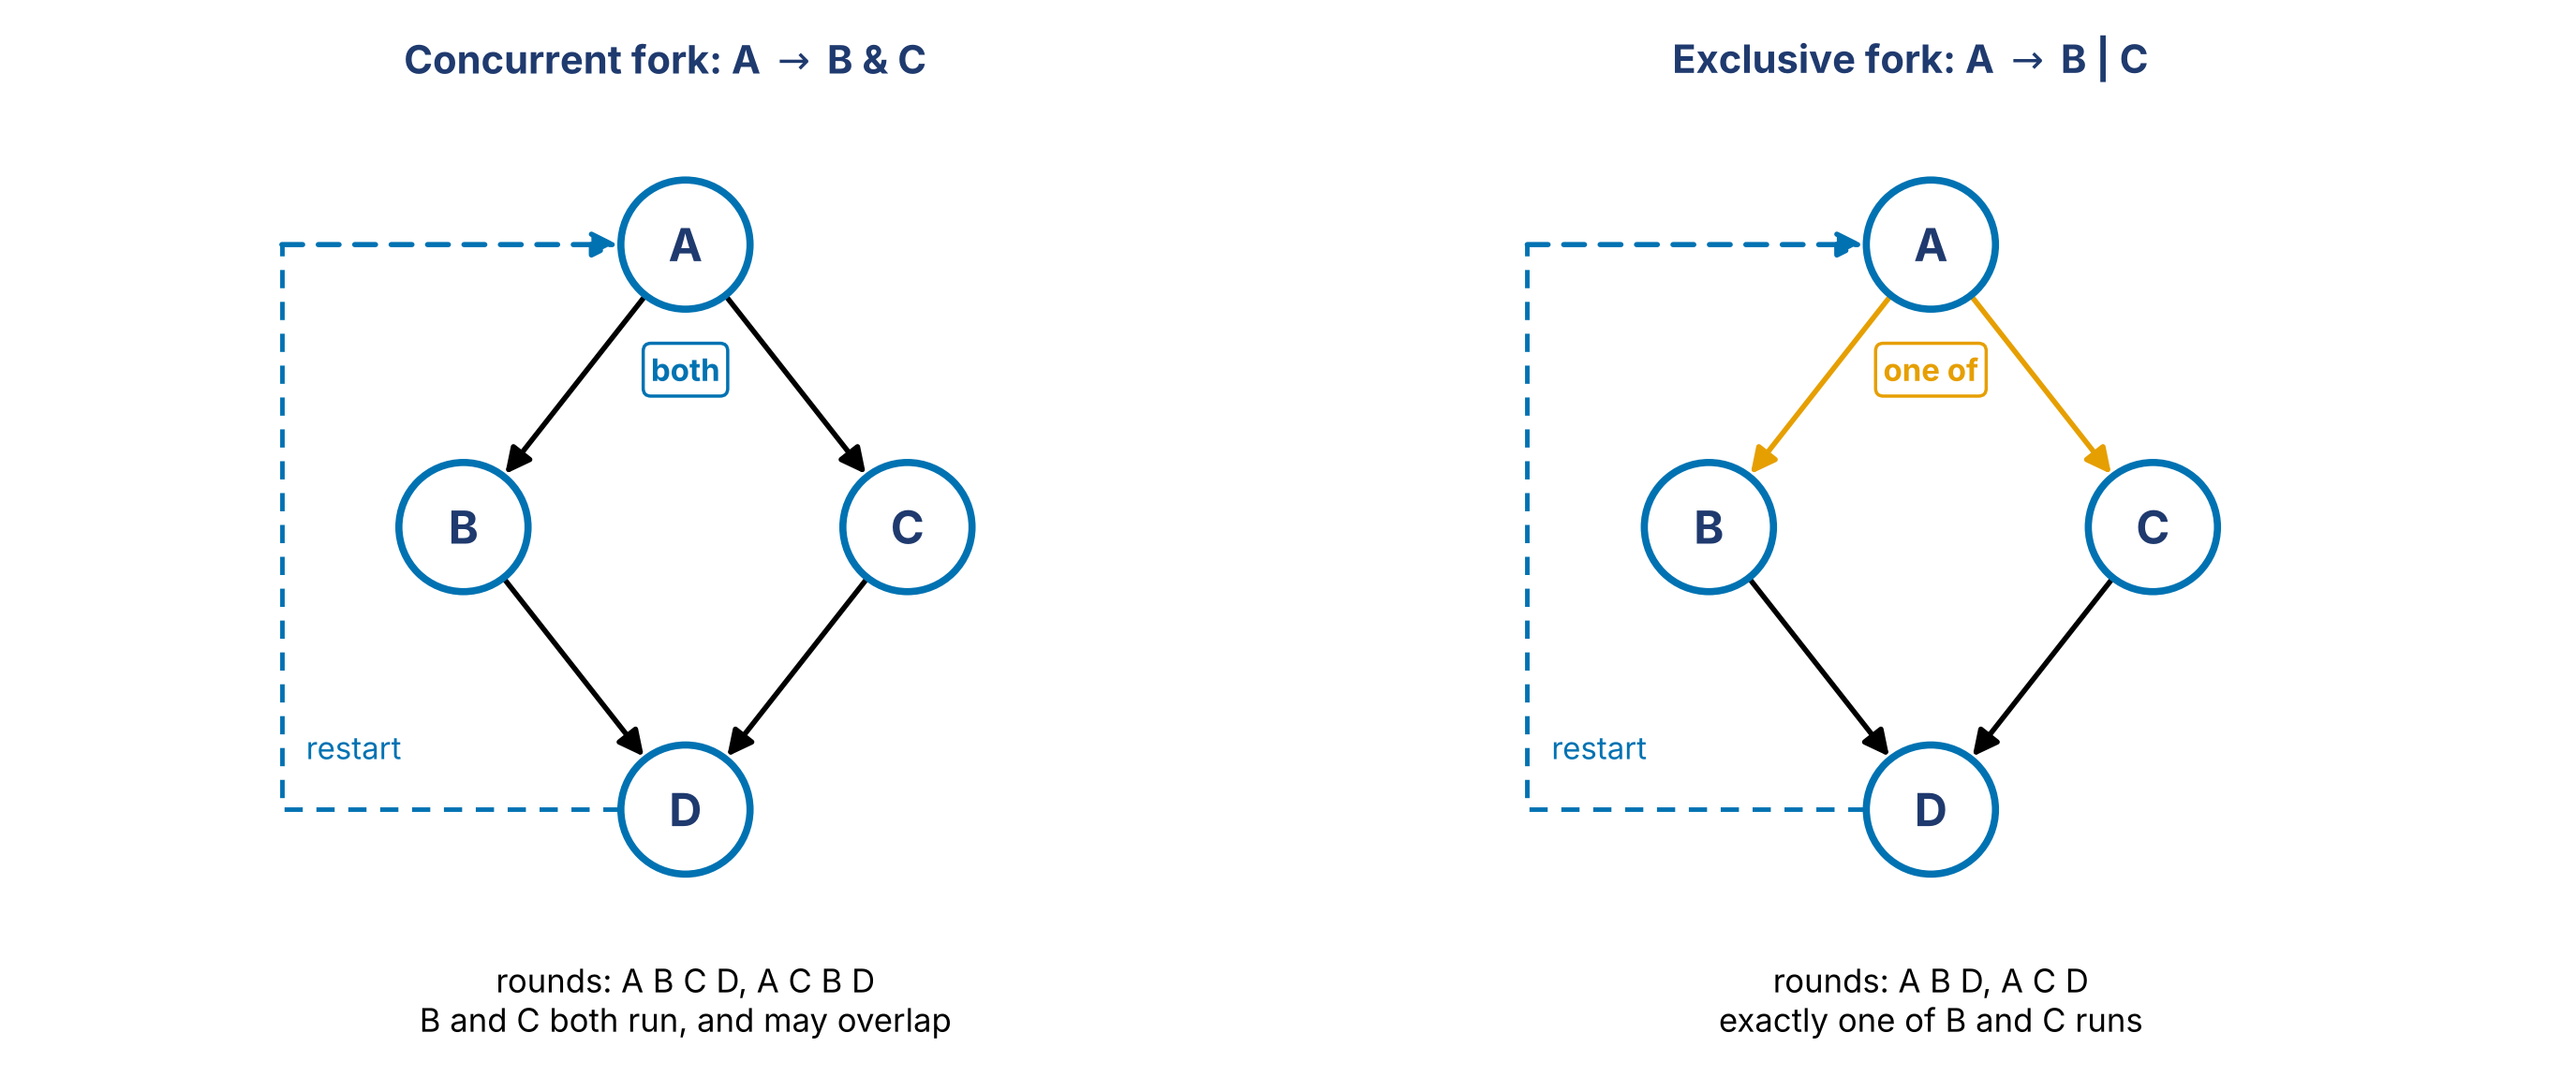
\includegraphics[width=0.95\textwidth]{contents/images/week-08/fork_two_meanings.png}
    \caption{The same four tasks and arrows, with the two meanings of the fork at A. The join at D and the dashed restart are the same in both.}
\end{figure}
\begin{itemize}
    \item \textbf{Concurrent fork}, A $\rightarrow$ B \& C (``both''): after A, \textbf{both} B and C run in every round, in any order, and their critical sections may overlap. D waits for both. Valid rounds: A B C D and A C B D.
    \item \textbf{Exclusive fork}, A $\rightarrow$ B $|$ C (``one of''): B and C are in mutual exclusion, and exactly \textbf{one} of them enters in each round. D waits for that one. Valid rounds: A B D and A C D.
    \item The arrows are the same: \textbf{the exercise must say which fork it means} (the slides write \texttt{\&} and \texttt{|}). At the exam, if it does not, raise your hand and ask; if in doubt, \textbf{write down the reading you used}.
\end{itemize}
The restart is not mandatory (some applications enforce an order only \textbf{once}), but almost every exercise has it.

\subsection{Three graphs}
Two skills. First, look at a graph and say whether a transition is legal: easy, but at the exam many errors are on very simple things. In Example 1, A $\rightarrow$ B and A $\rightarrow$ C are fine, even together; A followed directly by D is \textbf{wrong}. Second, always find the \textbf{forks} and the \textbf{joins}, because the semaphores go there: for each node count the edges that \textbf{leave} it (two or more: a fork) and those that \textbf{arrive} (two or more: a join).
\begin{figure}[H]
    \centering
    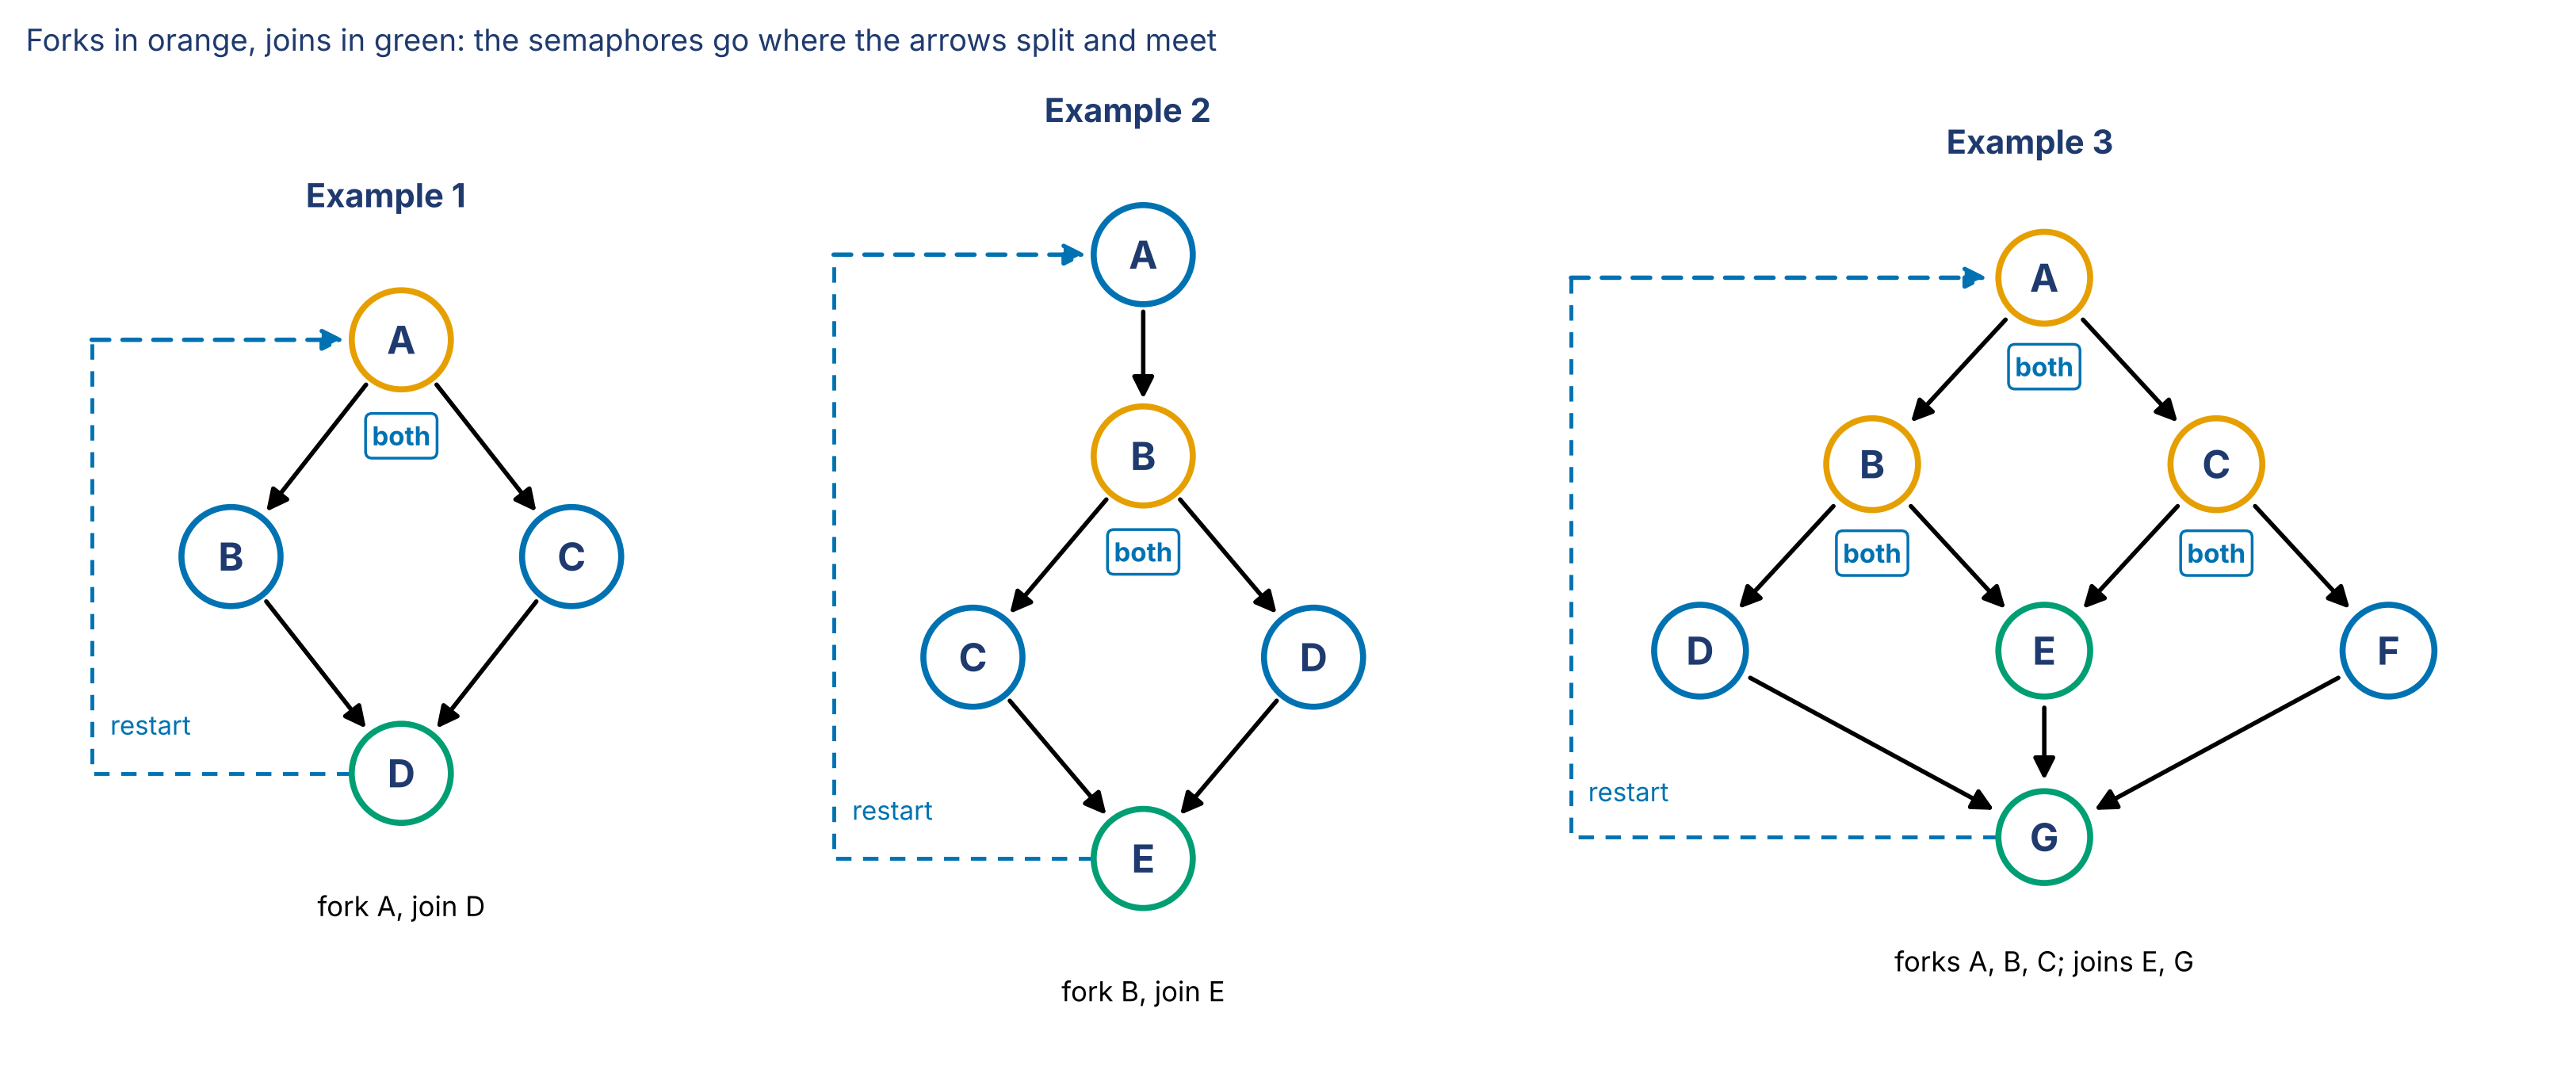
\includegraphics[width=1\textwidth]{contents/images/week-08/three_graphs.png}
    \caption{The three graphs of this unit. Every fork here is concurrent (``both''). Forks in orange, joins in green.}
\end{figure}
\begin{center}
\small
\begin{tabular}{l P{0.5} c c c}
    \hline
    & \textbf{edges} & \textbf{forks} & \textbf{joins} & \textbf{restart} \\
    \hline
    Example 1 & A$\rightarrow$B, A$\rightarrow$C, B$\rightarrow$D, C$\rightarrow$D & A & D & D$\rightarrow$A \\
    Example 2 & A$\rightarrow$B, B$\rightarrow$C, B$\rightarrow$D, C$\rightarrow$E, D$\rightarrow$E & B & E & E$\rightarrow$A \\
    Example 3 & A$\rightarrow$B, A$\rightarrow$C, B$\rightarrow$D, B$\rightarrow$E, C$\rightarrow$E, C$\rightarrow$F, D$\rightarrow$G, E$\rightarrow$G, F$\rightarrow$G & A, B, C & E, G & G$\rightarrow$A \\
    \hline
\end{tabular}
\end{center}

\subsection{The method: one semaphore per edge}
Every task has the same shape: an infinite loop; a \textbf{waiting} part, on some semaphores; the critical section; a \textbf{signalling} part, that tells the others they may go on. The whole problem is \textbf{how many} semaphores, which ones each task \textbf{waits} on, and which ones it \textbf{signals}. No general rule always gives the best answer, but this method always gives a correct one:
\begin{itemize}
    \item For each edge X $\rightarrow$ Y, a semaphore \texttt{sXY} that starts at \textbf{0} (``this round has not crossed the edge yet''): Y waits until X signals.
    \item The \textbf{restart} edge enters the first task, so its semaphore starts at \textbf{1}: that token lets the first round begin.
\end{itemize}
\begin{lstlisting}[basicstyle=\ttfamily\footnotesize]
X:  for ever:
        wait once on the semaphore of each incoming edge;
        critical section of X;
        signal once the semaphore of each outgoing edge;
\end{lstlisting}
Why it is correct, for concurrent forks:
\begin{itemize}
    \item \texttt{sXY} gets one token per round, after X finishes, so Y cannot enter before: the edge is respected.
    \item Each semaphore has exactly \textbf{one} task that signals and \textbf{one} that waits: a token cannot go to the wrong task.
    \item A \textbf{join waits for everything}: it passes its \texttt{wait}s in any order, and goes on only when it has them all; a token that arrives early simply stays in its semaphore.
    \item A task cannot run twice in a round: its token comes back only after the restart.
\end{itemize}
It is the \textbf{first thing to write in an exam}; reasoning on the specific case can then give fewer semaphores.

\paragraph{Example 1, concurrent, one semaphore per edge.} Four edges and the restart: five semaphores. On the left the paper program; on the right its translation, shown for A.
\begin{figure}[H]
    \centering
    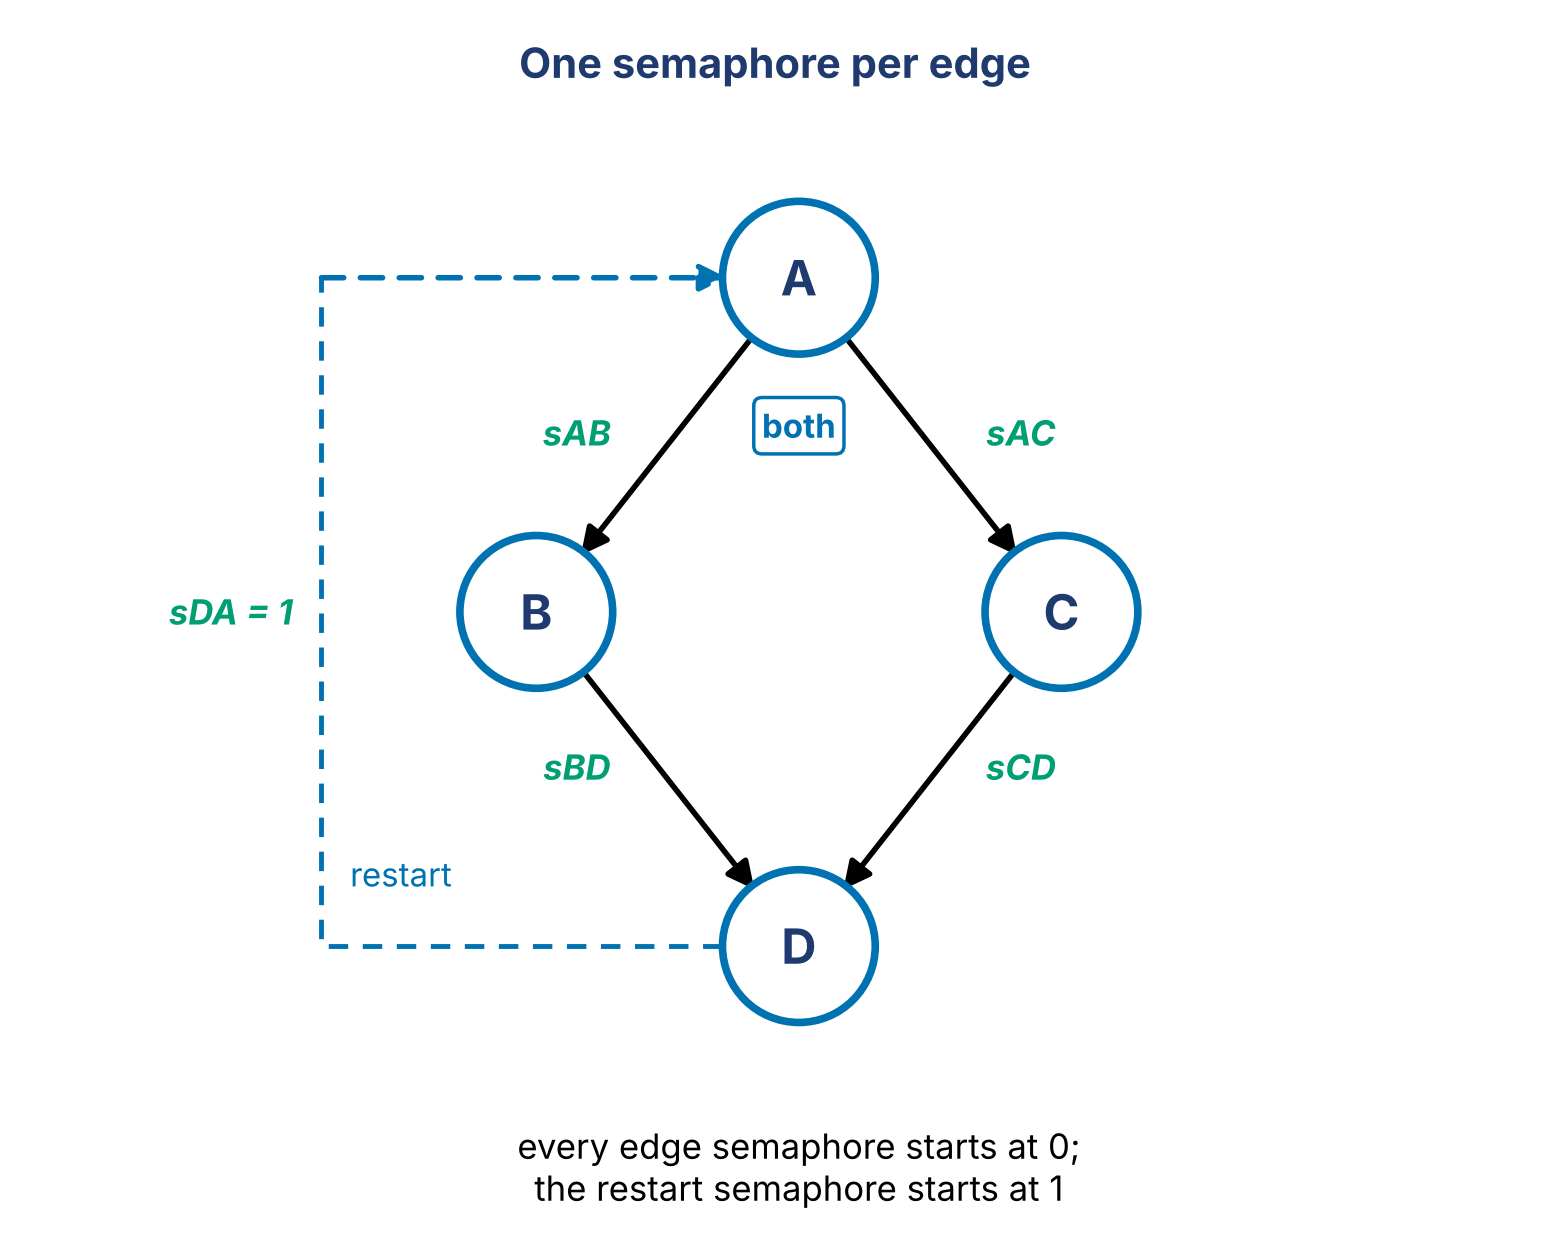
\includegraphics[width=0.5\textwidth]{contents/images/week-08/example1_edges.png}
    \caption{Example 1 with one semaphore per edge: four edges and the restart, so five semaphores.}
\end{figure}
\par\noindent\begin{minipage}[t]{0.44\textwidth}
\begin{lstlisting}[basicstyle=\ttfamily\scriptsize]
semaphore sDA = 1, sAB = 0, sAC = 0,
          sBD = 0, sCD = 0;

A: for ever:
     wait( sDA );
     CS A
     signal( sAB ); signal( sAC );
B: for ever:
     wait( sAB ); CS B; signal( sBD );
C: for ever:
     wait( sAC ); CS C; signal( sCD );
D: for ever:
     wait( sBD ); wait( sCD );
     CS D
     signal( sDA );
\end{lstlisting}
\end{minipage}\hfill
\begin{minipage}[t]{0.5\textwidth}
\begin{lstlisting}[language=C, showstringspaces=false, basicstyle=\ttfamily\scriptsize]
/* sDA starts at 1, with a maximum of 1 */
sDA = xSemaphoreCreateCounting( 1, 1 );
/* the others: xSemaphoreCreateBinary() */

/* A */
for( ;; )
{
    xSemaphoreTake( sDA, portMAX_DELAY );
    critical_section();
    xSemaphoreGive( sAB );
    xSemaphoreGive( sAC );
}
\end{lstlisting}
\end{minipage}
\begin{itemize}
    \item Valid rounds: A B C D and A C B D. A is first, because everything depends on it; D is last, because it needs B and C; nothing orders B and C.
    \item \textbf{A} waits on the restart \texttt{sDA} and signals \textbf{both} outgoing edges, because B and C run concurrently (mutual exclusion changes the scheme, below). \textbf{B} and \textbf{C} wait on their edge from A and signal their edge to D. \textbf{D}, a join, waits on \textbf{both} and signals the restart.
    \item In FreeRTOS each call becomes one call; only the \textbf{creation} needs care. The edge semaphores hold 0 or 1, so they can be binary; \texttt{sDA} starts at 1, which a binary semaphore cannot do, so it is counting with maximum 1\footnote{In class the professor first said ``binary'' for it, then corrected himself: a FreeRTOS binary semaphore always starts at 0.}. From now on these notes show the paper notation, and for FreeRTOS only the creation.
\end{itemize}

\subsection{Fewer semaphores: same end yes, same start no}
Semaphores are kernel objects: they cost \textbf{memory} and \textbf{scheduling effort}, so it pays to remove some. But a semaphore has \textbf{no names on its tokens}: a signal just adds 1, and nobody remembers which task added it. Two ways to merge edges look alike, but in a loop they behave differently.
\begin{itemize}
    \item \textbf{Same end (join share): safe.} B $\rightarrow$ D and C $\rightarrow$ D share \texttt{sD}. B and C each signal it \textbf{once} (counting, it can reach 2), and D waits \textbf{twice}, so both must have run. B cannot give a second token instead of C: it cannot run again before the restart, which comes after D.
    \item \textbf{Same start (fork share): wrong.} A $\rightarrow$ B and A $\rightarrow$ C share \texttt{sF}, and A signals it \textbf{twice}, one token for B and one for C. The count is right, but there is no label on a token.
\end{itemize}
\paragraph{The trap: a task steals the token of its sibling.} With \texttt{sF} shared, find a round in which C never runs:
\begin{lstlisting}[basicstyle=\ttfamily\footnotesize]
A:  for ever:  wait( sA );  CS A;  signal( sF );  signal( sF );
B:  for ever:  wait( sF );  CS B;  signal( sD );
C:  for ever:  wait( sF );  CS C;  signal( sD );
D:  for ever:  wait( sD );  wait( sD );  CS D;  signal( sA );
\end{lstlisting}
\begin{figure}[H]
    \centering
    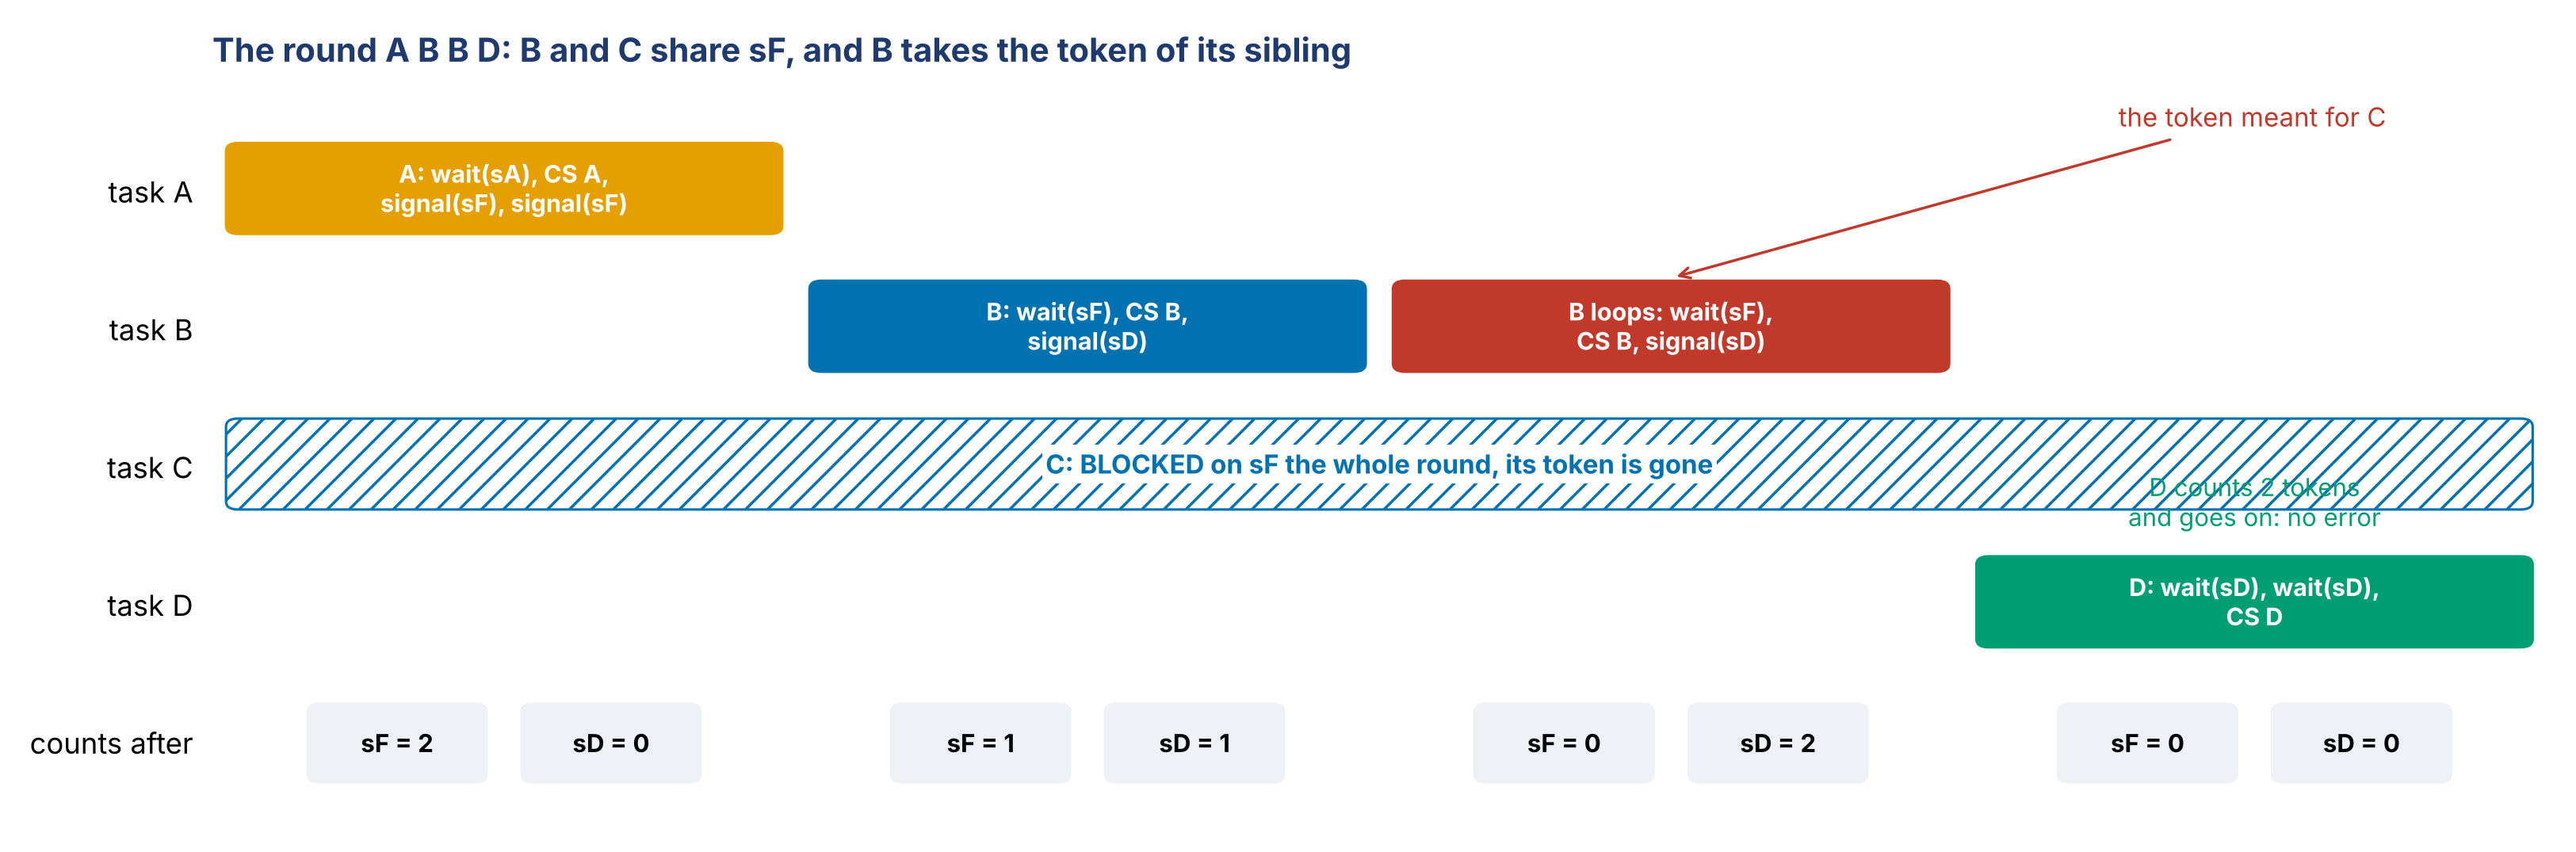
\includegraphics[width=0.95\textwidth]{contents/images/week-08/token_steal.png}
    \caption{The round A B B D. After its critical section B is back at the top of its loop, one more task waiting on \texttt{sF}, and it takes the token meant for C. Nothing reports an error: D counts two tokens and goes on.}
\end{figure}
If each task ran only once, this sharing would be fine: the \textbf{infinite loop} breaks it. Nothing blocks and no error appears, so this bug is \textbf{easy to miss}; you see it run in Unit 2. A signal cannot say ``this one is for C'': the only way is \textbf{separate semaphores}.
\begin{center}
\fbox{\parbox{0.9\textwidth}{\centering\textbf{Rule}: two tasks that must both run in a round never wait on the same semaphore.\\ So a concurrent fork gives each branch its own semaphore; sharing is safe at a join.}}
\end{center}
\paragraph{At the exam.} (The question everybody had and was too shy to ask.) The solution of the method works and is accepted; the \textbf{optimal} one gets more points, a less optimal one loses a few, a \textbf{wrong} one gets zero or little. If you are confident, optimise; if not, the mechanical method is the bottom level, and at least you get there.

\subsection{Example 1 with the fewest semaphores}
\paragraph{Concurrent: four semaphores.} One semaphore per task, named after it; only the join is shared.
\par\noindent\begin{minipage}[t]{0.47\textwidth}
\begin{lstlisting}[basicstyle=\ttfamily\scriptsize]
semaphore sA = 1, sB = 0, sC = 0, sD = 0;

A: for ever:
     wait( sA );
     CS A
     signal( sB ); signal( sC );
B: for ever:
     wait( sB ); CS B; signal( sD );
C: for ever:
     wait( sC ); CS C; signal( sD );
D: for ever:
     wait( sD ); wait( sD );
     CS D
     signal( sA );
\end{lstlisting}
\end{minipage}\hfill
\begin{minipage}[t]{0.49\textwidth}
\begin{lstlisting}[language=C, showstringspaces=false, basicstyle=\ttfamily\scriptsize]
sA = xSemaphoreCreateCounting( 1, 1 );
sB = xSemaphoreCreateBinary();
sC = xSemaphoreCreateBinary();
sD = xSemaphoreCreateCounting( 2, 0 );
\end{lstlisting}
\raggedright Each task waits only on its own semaphore, once per incoming edge. \texttt{sD} carries B $\rightarrow$ D and C $\rightarrow$ D: it is \textbf{counting}, because B and C may both finish before D takes a token. Valid rounds as before.
\end{minipage}

\paragraph{Exclusive: three semaphores.} Now A $\rightarrow$ B $|$ C: after the fork only \textbf{one} task must become executable. Put \textbf{one} semaphore, and let A signal it \textbf{once}: the first of B and C that is scheduled takes the token. Here sharing is exactly what we want: one token, two tasks that want it.
\begin{lstlisting}[basicstyle=\ttfamily\footnotesize]
semaphore sA = 1, sF = 0, sD = 0;

A:  for ever:  wait( sA );  CS A;  signal( sF );
B:  for ever:  wait( sF );  CS B;  signal( sD );
C:  for ever:  wait( sF );  CS C;  signal( sD );
D:  for ever:  wait( sD );  CS D;  signal( sA );
\end{lstlisting}
\begin{itemize}
    \item Valid rounds: A B D and A C D. The next token on \texttt{sF} comes only after the restart, so the task that has just run may compete for it again, but cannot run twice in a round.
    \item \textbf{Which one wins is not fixed}: the waiting tasks sit in a queue, and the scheduler decides who goes back to running. Mutual exclusion imposes no B-then-C alternation: A B D a hundred times in a row only means a very bad scheduler, and the synchronization is still correct. One of them may even \textbf{never} run (Unit 2).
    \item \textbf{D waits once}, on a shared \texttt{sD} signalled by both B and C. \emph{Why is it safe?} (A question from the class.) D cannot run right after A, because only B or C signal \texttt{sD}; it cannot run twice, because only one of B and C runs in a round, so \texttt{sD} never exceeds 1.
\end{itemize}
\begin{center}
\small
\begin{tabular}{l P{0.27} P{0.27} P{0.15}}
    \hline
    & \textbf{A signals} & \textbf{B and C wait on} & \textbf{D waits} \\
    \hline
    concurrent & two different semaphores & their own semaphore & twice \\
    exclusive & one semaphore, once & the same semaphore & once \\
    \hline
\end{tabular}
\end{center}

\subsection{Try it on paper: small mistakes in Example 1}
Each change below is one line different from a correct solution. What goes wrong?
\begin{enumerate}
    \item Concurrent: \texttt{sA} starts at 0.
    \item Concurrent: D waits on \texttt{sD} only once.
    \item Concurrent, in FreeRTOS: \texttt{sD} is created with \texttt{xSemaphoreCreateBinary()}, and both B and C give it before D takes.
    \item Exclusive: A signals \texttt{sF} twice.
    \item Exclusive: D waits on \texttt{sD} twice.
\end{enumerate}
\needspace{4\baselineskip}
\textbf{Solution.}
\begin{enumerate}
    \item \textbf{Nothing ever runs.} Every task waits for a token, and no task can give the first one. The system stops at once, with no error.
    \item \textbf{D does not wait for both.} D passes after the first \texttt{signal( sD )}, so the round A B D is possible, with C still to come. It breaks C $\rightarrow$ D, and the restart can start a new round on top of the old one.
    \item \textbf{A binary semaphore holds at most 1.} The second give finds it full and returns \texttt{pdFALSE}, and the token is lost. D waits for ever, so A does too. The bug appears only when D has not taken the first token before the second give, so it can stay hidden for a long time: it is the maximum, the difference between paper and FreeRTOS.
    \item \textbf{Both branches can run.} With two tokens the round A B C is possible, which breaks the ``one of''. D then has a token left over, so in the next round D can enter too early.
    \item \textbf{The first round never ends.} Only one branch runs, so the second token never arrives. D waits for ever, and the whole cycle stops.
\end{enumerate}

\subsection{Example 2: the same arrows, two meanings}
\begin{figure}[H]
    \centering
    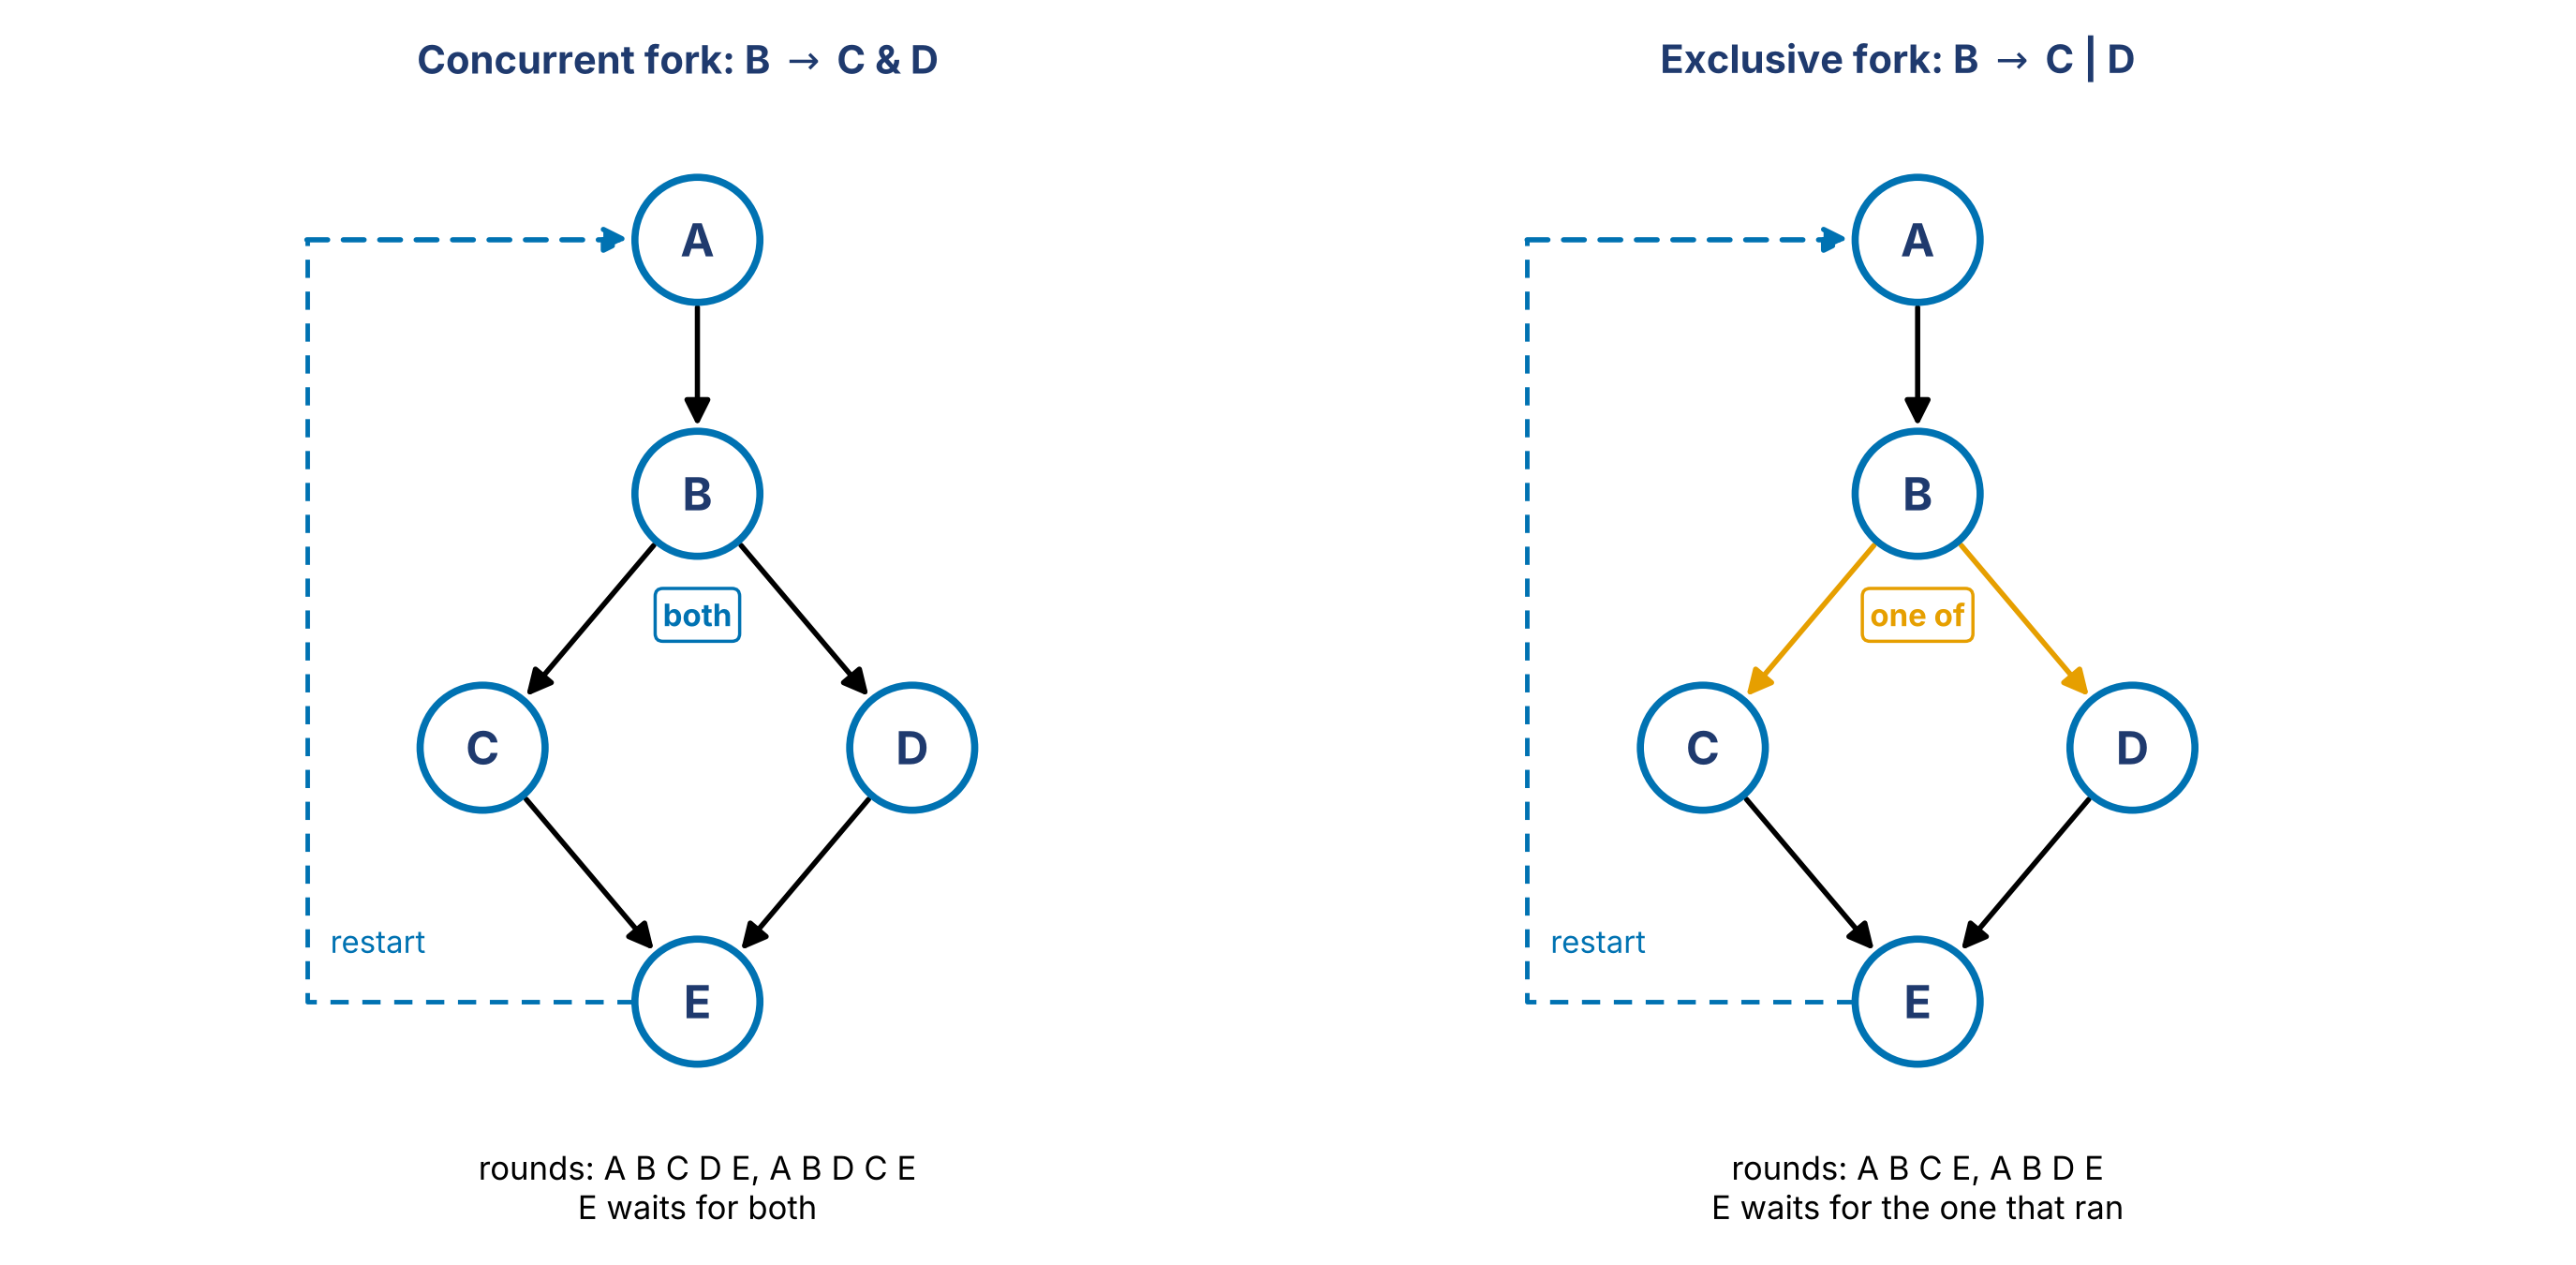
\includegraphics[width=0.72\textwidth]{contents/images/week-08/example2_forks.png}
    \caption{Example 2 drawn twice: A and B run in every round; the fork at B decides what E waits for.}
\end{figure}
With a concurrent fork the method gives six semaphores (five edges and the restart); here are the fewest.
\par\noindent\begin{minipage}[t]{0.49\textwidth}
\textbf{Concurrent}, five semaphores:
\begin{lstlisting}[basicstyle=\ttfamily\scriptsize]
semaphore sA = 1, sB = 0, sC = 0,
          sD = 0, sE = 0;

A: for ever: wait( sA ); CS A; signal( sB );
B: for ever: wait( sB ); CS B;
             signal( sC ); signal( sD );
C: for ever: wait( sC ); CS C; signal( sE );
D: for ever: wait( sD ); CS D; signal( sE );
E: for ever: wait( sE ); wait( sE );
             CS E; signal( sA );
\end{lstlisting}
\texttt{sE} is counting, with a maximum of 2.
\end{minipage}\hfill
\begin{minipage}[t]{0.49\textwidth}
\textbf{Exclusive}, four semaphores:
\begin{lstlisting}[basicstyle=\ttfamily\scriptsize]
semaphore sA = 1, sB = 0, sF = 0, sE = 0;

A: for ever: wait( sA ); CS A; signal( sB );
B: for ever: wait( sB ); CS B; signal( sF );
C: for ever: wait( sF ); CS C; signal( sE );
D: for ever: wait( sF ); CS D; signal( sE );
E: for ever: wait( sE ); CS E; signal( sA );
\end{lstlisting}
All binary, apart from \texttt{sA}, which starts at 1.
\end{minipage}

\medskip
The difference is in B (two semaphores, or one shared), in C and D (their own semaphore, or the shared one) and in E (waits twice, or once). The professor calls this a \textbf{very important slide}: it has almost everything that can happen, a fork, a join and the two kinds of fork. A bigger graph is a \textbf{combination of these patterns}.

\subsection{How few semaphores can there be?}
\begin{figure}[H]
    \centering
    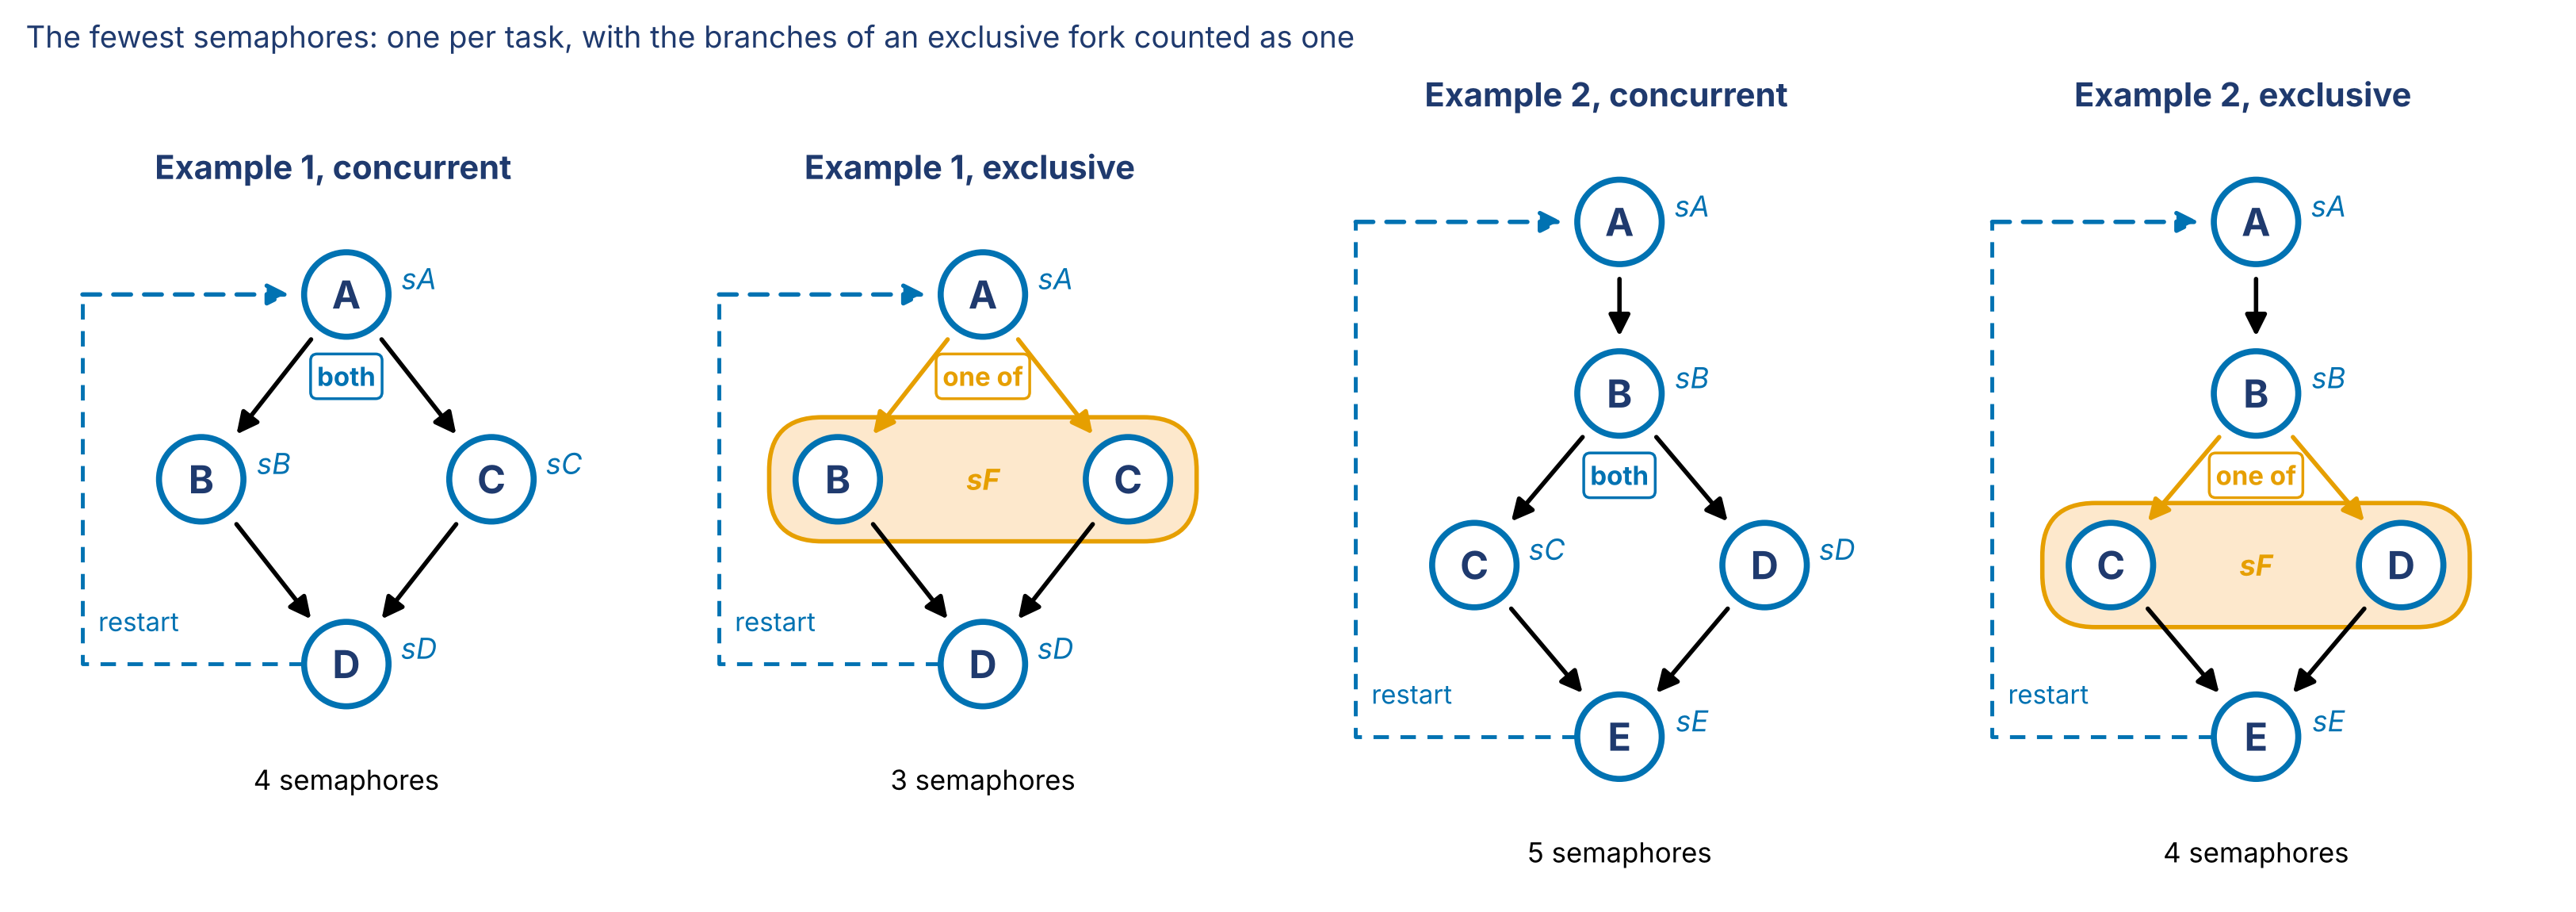
\includegraphics[width=1\textwidth]{contents/images/week-08/fewest_semaphores.png}
    \caption{Examples 1 and 2, concurrent and exclusive, with the fewest semaphores: each task has its own; only the two branches of an exclusive fork share one (\texttt{sF}).}
\end{figure}
Two tasks that must both run in a round cannot wait on the same semaphore; only the branches of one exclusive fork may share. So:
\begin{center}
\fbox{\parbox{0.9\textwidth}{\centering\textbf{The fewest semaphores}: one per task, with the branches of one exclusive fork counted as one.}}
\end{center}
That gives 4 and 3 semaphores for Example 1, 5 and 4 for Example 2. Each task waits on its own semaphore once per incoming edge (once for an exclusive join); the maximum of a counting semaphore is the number of tokens that can wait in it. The minimum holds for programs of this form (wait, enter, signal): a program that lists all the runs of every solution with one semaphore less finds no correct one.
\begin{itemize}
    \item For every exercise: find the forks and the joins, and know whether each fork is concurrent or exclusive. If the exam does not say, \textbf{ask}: without it the exercise cannot be solved.
    \item Forks may have more than two branches, with the same meaning: concurrent, all run; exclusive, exactly one.
    \item The mechanism is simple, but easy to confuse: practise until it is clear, because at the exam stress makes the mind work less well, and the only defence is knowing the topic very well.
\end{itemize}

\subsection{Example 3}
\paragraph{Read the graph first.} A bigger graph makes the \textbf{understanding} harder, not the solution: write down what each task really needs before writing any semaphore.
\begin{center}
\small
\begin{tabular}{c c c}
    \hline
    \textbf{task} & \textbf{waits for} & \textbf{enables} \\
    \hline
    A & restart & B, C \\
    B & A & D, E \\
    C & A & E, F \\
    D & B & G \\
    E & B and C & G \\
    F & C & G \\
    G & D, E and F & restart \\
    \hline
\end{tabular}
\end{center}
Every fork is concurrent; nine edges and the restart. Only E needs both B and C: D does \textbf{not} need C, and F does \textbf{not} need B. A is always first and G always last. Are \textbf{A C F B D E G} and \textbf{A B D E C F G} valid rounds?
\begin{itemize}
    \item \textbf{A C F B D E G is valid}: check its edges one by one (F needs only C; D needs B; E needs B and C, both done; G needs D, E, F).
    \item \textbf{A B D E C F G is not}: E runs before C, and it breaks C $\rightarrow$ E.
    \item Read the graph by its \textbf{edges}, not by layers: even the professor, going too fast, hesitated on the first sequence. Some automotive applications run 30 to 50 tasks with much more complex graphs.
\end{itemize}

\paragraph{From ten semaphores to seven.} The method gives ten; one semaphore per task gives seven:
\par\noindent\begin{minipage}[t]{0.55\textwidth}
\begin{lstlisting}[basicstyle=\ttfamily\scriptsize]
semaphore sA = 1, sB = 0, sC = 0, sD = 0,
          sE = 0, sF = 0, sG = 0;

A: for ever: wait( sA ); CS A;
             signal( sB ); signal( sC );
B: for ever: wait( sB ); CS B;
             signal( sD ); signal( sE );
C: for ever: wait( sC ); CS C;
             signal( sE ); signal( sF );
D: for ever: wait( sD ); CS D; signal( sG );
E: for ever: wait( sE ); wait( sE );
             CS E; signal( sG );
F: for ever: wait( sF ); CS F; signal( sG );
G: for ever: wait( sG ); wait( sG ); wait( sG );
             CS G; signal( sA );
\end{lstlisting}
\end{minipage}\hfill
\begin{minipage}[t]{0.42\textwidth}
\begin{lstlisting}[language=C, showstringspaces=false, basicstyle=\ttfamily\scriptsize]
sA = xSemaphoreCreateCounting( 1, 1 );
sB = xSemaphoreCreateBinary();
sC = xSemaphoreCreateBinary();
sD = xSemaphoreCreateBinary();
sE = xSemaphoreCreateCounting( 2, 0 );
sF = xSemaphoreCreateBinary();
sG = xSemaphoreCreateCounting( 3, 0 );
\end{lstlisting}
\raggedright The maximum of a counting semaphore is the \textbf{number of its incoming edges}. E waits twice on \texttt{sE}: B and C each give one per round, so the two tokens are one of each. Listing all the runs finds only valid rounds.
\end{minipage}

\paragraph{A tempting solution.} ``B and C each give two tokens; D, E and F take the tokens they need'': one semaphore \texttt{sM} for the whole middle level.
\begin{lstlisting}[basicstyle=\ttfamily\footnotesize]
semaphore sR = 1, sA = 0, sM = 0, sG = 0;

A:  for ever:  wait( sR );  CS A;  signal( sA );  signal( sA );
B:  for ever:  wait( sA );  CS B;  signal( sM );  signal( sM );
C:  for ever:  wait( sA );  CS C;  signal( sM );  signal( sM );
D:  for ever:  wait( sM );  CS D;  signal( sG );
E:  for ever:  wait( sM );  wait( sM );  CS E;  signal( sG );
F:  for ever:  wait( sM );  CS F;  signal( sG );
G:  for ever:  wait( sG );  wait( sG );  wait( sG );  CS G;  signal( sR );
\end{lstlisting}
The count is right: 4 tokens given, 4 taken. Find two different mistakes, using the runs it allows.
\needspace{3\baselineskip}
\textbf{Solution.} On both \texttt{sA} and \texttt{sM}, several tasks that must all run wait together. \textbf{The steal}: A B B, because B can loop and take the token of C on \texttt{sA}. \textbf{The wrong token}: A B E, because E can take the two tokens of B and enter before C, which breaks C $\rightarrow$ E: two tokens of B look just like one of B and one of C. \textbf{Testing can miss this}: if the priorities happen to run C early, the bad order never shows up. Reason about \textbf{every} possible run, never trust one run. The professor prepared many more examples to review at home, many of them \textbf{wrong} solutions from very common mistakes: the temptation to remove semaphores is exactly where the errors are.

\subsection{Try it on paper: precedence graphs}
Exercises to practise for the exam, as in the slides. Unless stated, write \texttt{wait}/\texttt{signal}, with the fewest semaphores.

\paragraph{Your turn.} A $\rightarrow$ B \& C, B $\rightarrow$ D $|$ E, then D$\rightarrow$F, E$\rightarrow$F, C$\rightarrow$G, F$\rightarrow$G, and the restart G$\rightarrow$A.
\par\noindent\begin{minipage}[c]{0.42\textwidth}
\centering
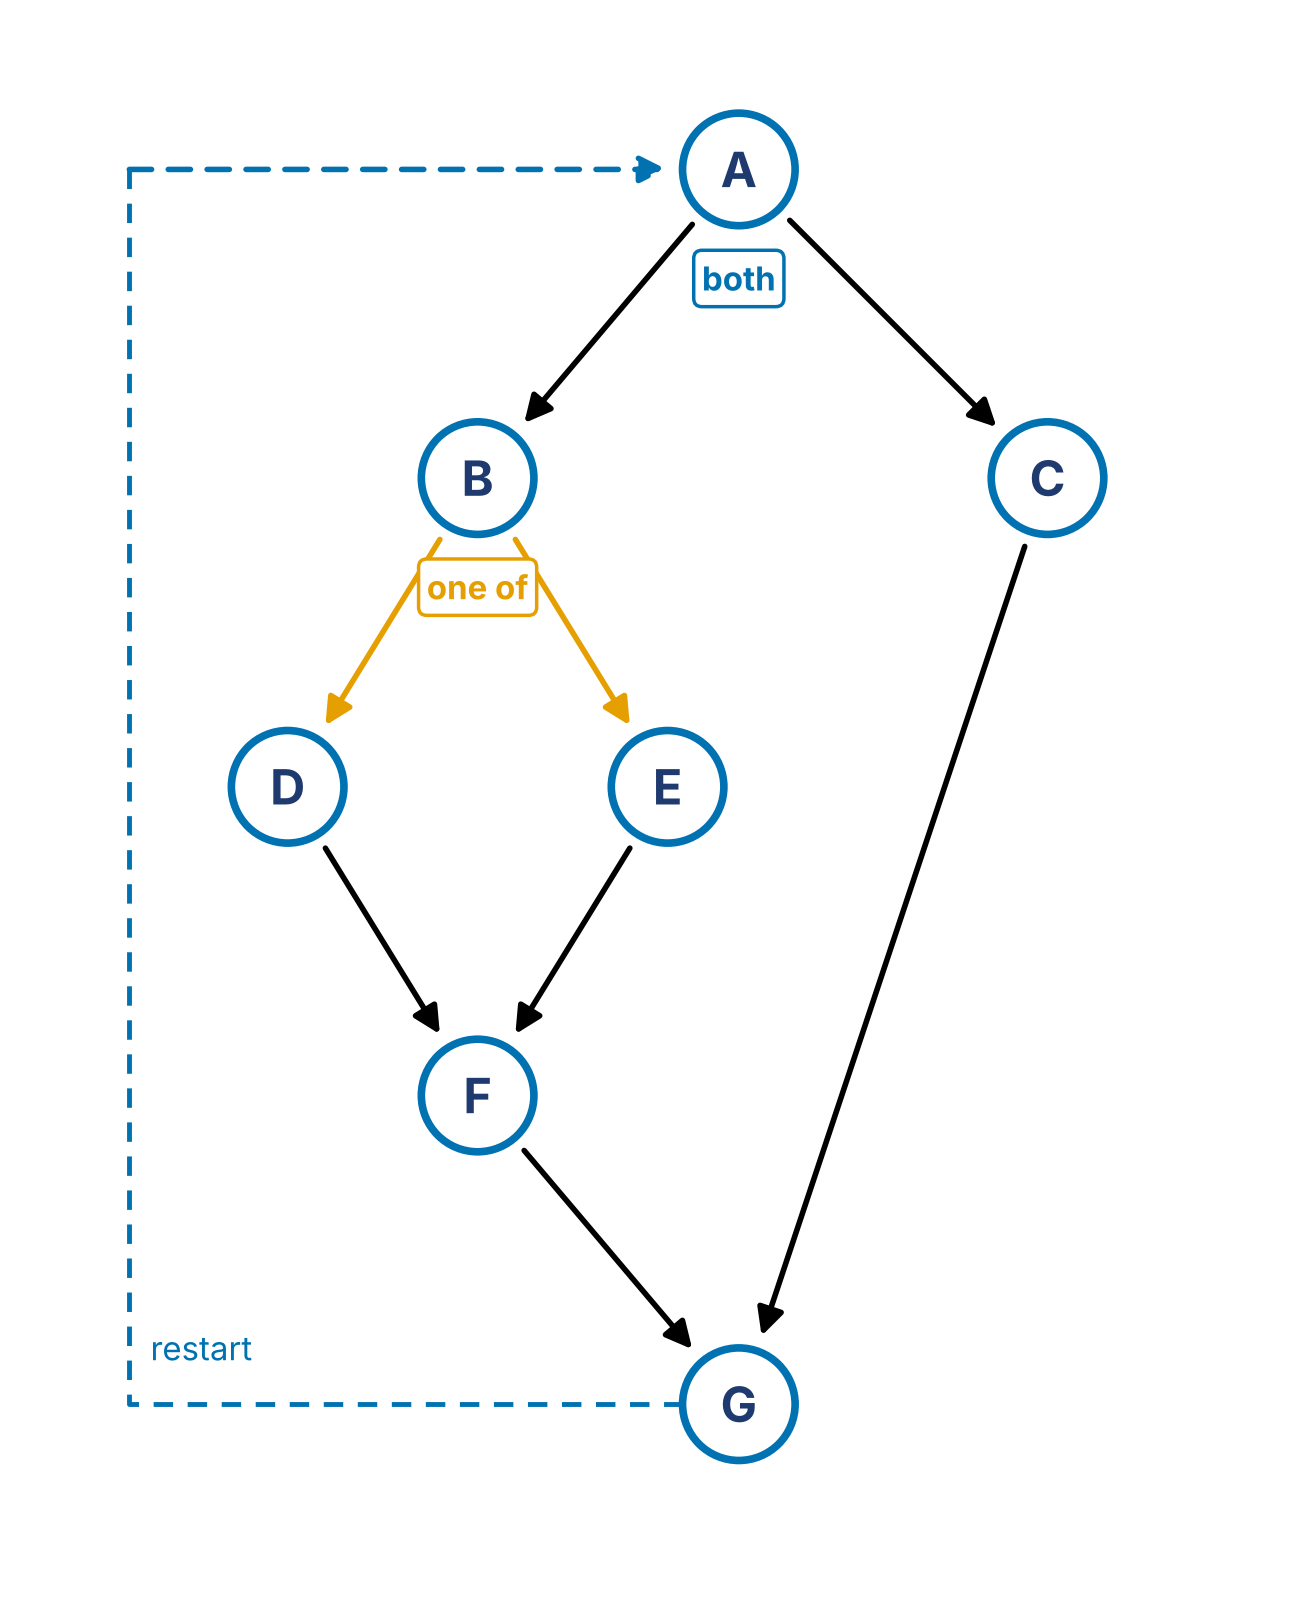
\includegraphics[width=0.85\textwidth]{contents/images/week-08/ex_your_turn.png}
\end{minipage}\hfill
\begin{minipage}[c]{0.55\textwidth}
\begin{enumerate}
    \item Which tasks run in every round? Which do not?
    \item Give two valid rounds, and one order that is not valid. Which edge does it break?
    \item Write the solution with the fewest semaphores.
    \item Which semaphores must be counting in FreeRTOS, and with which maximum? Which one starts at 1?
\end{enumerate}
\end{minipage}
\needspace{4\baselineskip}
\textbf{Solution.}
\begin{enumerate}
    \item A, B, C, F and G run in every round. D and E are exclusive: exactly one of them runs.
    \item A B D F C G and A C B E F G are valid. A B D F G C is not: G runs before C, and it breaks C $\rightarrow$ G. A B D E F C G is not either: D and E both run, and the fork at B allows only one.
    \item Six semaphores: seven tasks, with D and E counted as one.
\begin{lstlisting}[basicstyle=\ttfamily\scriptsize]
semaphore sA = 1, sB = 0, sC = 0, sX = 0, sF = 0, sG = 0;

A: for ever: wait( sA ); CS A; signal( sB ); signal( sC );
B: for ever: wait( sB ); CS B; signal( sX );
C: for ever: wait( sC ); CS C; signal( sG );
D: for ever: wait( sX ); CS D; signal( sF );
E: for ever: wait( sX ); CS E; signal( sF );
F: for ever: wait( sF ); CS F; signal( sG );
G: for ever: wait( sG ); wait( sG ); CS G; signal( sA );
\end{lstlisting}
    \item \texttt{sG} is counting with a maximum of 2, because C and F may both finish first. \texttt{sA} starts at 1: \texttt{xSemaphoreCreateCounting( 1, 1 )}. The others can be binary. Note the two waits: G waits twice because of the concurrent fork at A, and F waits once because of the exclusive fork at B.
\end{enumerate}

\paragraph{Add the semaphores (1).} The tasks are written; add the semaphores so that they follow the graph, with as few as possible: the declaration with the initial values, and the \texttt{wait} and \texttt{signal} calls around each \texttt{CS}. Which semaphores must be counting in FreeRTOS?
\begin{center}
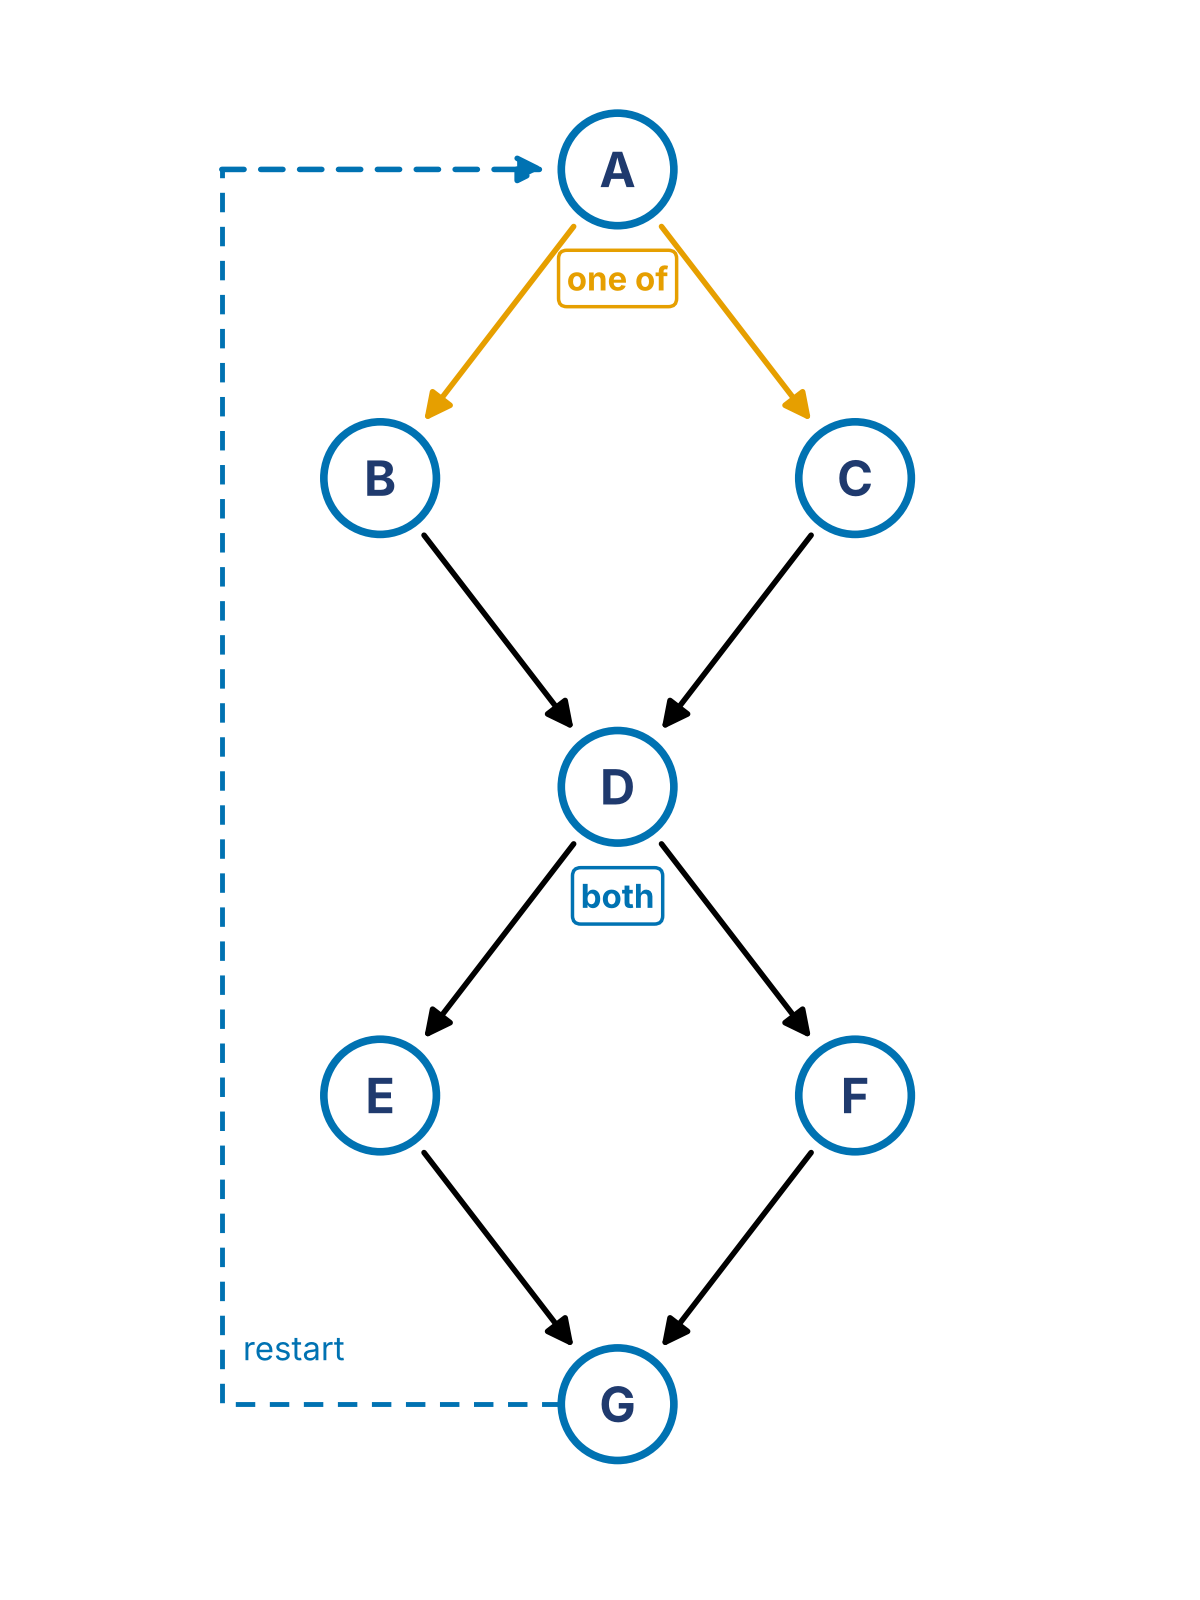
\includegraphics[width=0.33\textwidth]{contents/images/week-08/ex_add1.png}
\end{center}
\needspace{4\baselineskip}
\textbf{Solution.} Six semaphores: seven tasks, with B and C counted as one.
\begin{lstlisting}[basicstyle=\ttfamily\scriptsize]
semaphore sA = 1, sX = 0, sD = 0, sE = 0, sF = 0, sG = 0;

A: for ever: wait( sA );              CS A; signal( sX );
B: for ever: wait( sX );              CS B; signal( sD );
C: for ever: wait( sX );              CS C; signal( sD );
D: for ever: wait( sD );              CS D; signal( sE ); signal( sF );
E: for ever: wait( sE );              CS E; signal( sG );
F: for ever: wait( sF );              CS F; signal( sG );
G: for ever: wait( sG ); wait( sG );  CS G; signal( sA );
\end{lstlisting}
\begin{itemize}
    \item The fork at A is exclusive: A signals once, and B and C wait on the same semaphore. D waits once, because only one of them ran.
    \item The fork at D is concurrent: D signals two semaphores, and E and F each wait on their own. G waits twice, because both ran.
    \item \texttt{sG} is counting, with a maximum of 2. \texttt{sA} starts at 1, so in FreeRTOS it is \texttt{xSemaphoreCreateCounting( 1, 1 )}.
\end{itemize}

\paragraph{Add the semaphores (2), in FreeRTOS.} Q runs in every round, together with one of R and S. Declare and create the semaphores (\texttt{SemaphoreHandle\_t}), and write the \texttt{xSemaphoreTake} and \texttt{xSemaphoreGive} calls around each \texttt{cs()}, the critical section of the task.
\begin{center}
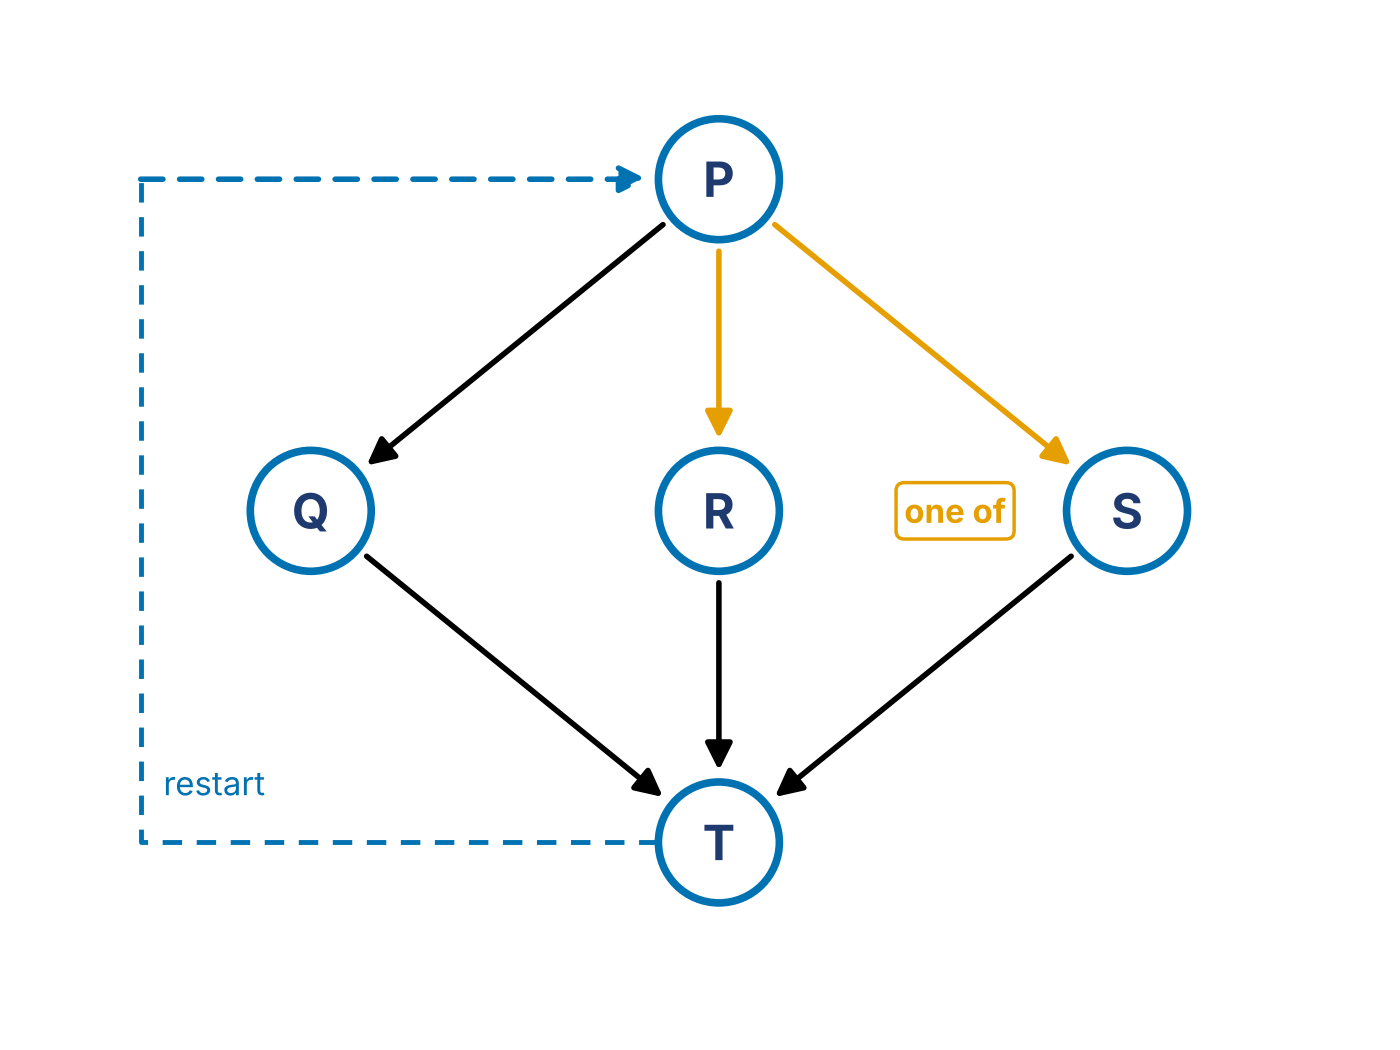
\includegraphics[width=0.42\textwidth]{contents/images/week-08/ex_add2.png}
\end{center}
\needspace{4\baselineskip}
\textbf{Solution.}
\par\noindent\begin{minipage}[t]{0.5\textwidth}
\begin{lstlisting}[language=C, showstringspaces=false, basicstyle=\ttfamily\scriptsize]
SemaphoreHandle_t sP, sQ, sX, sT;

sP = xSemaphoreCreateCounting( 1, 1 );
sQ = xSemaphoreCreateBinary();
sX = xSemaphoreCreateBinary();
sT = xSemaphoreCreateCounting( 2, 0 );

/* P */ for( ;; )
{
    xSemaphoreTake( sP, portMAX_DELAY );
    cs();
    xSemaphoreGive( sQ );
    xSemaphoreGive( sX );
}
\end{lstlisting}
\end{minipage}\hfill
\begin{minipage}[t]{0.47\textwidth}
\begin{lstlisting}[language=C, showstringspaces=false, basicstyle=\ttfamily\scriptsize]
/* Q */ for( ;; )
{
    xSemaphoreTake( sQ, portMAX_DELAY );
    cs();
    xSemaphoreGive( sT );
}
/* R and S: the same code */ for( ;; )
{
    xSemaphoreTake( sX, portMAX_DELAY );
    cs();
    xSemaphoreGive( sT );
}
/* T */ for( ;; )
{
    xSemaphoreTake( sT, portMAX_DELAY );
    xSemaphoreTake( sT, portMAX_DELAY );
    cs();
    xSemaphoreGive( sP );
}
\end{lstlisting}
\end{minipage}

\noindent R and S share \texttt{sX}, with one token per round, because they are exclusive; Q has its own semaphore, because it always runs. T takes twice, although three tasks can give \texttt{sT}: only two of them run in a round, Q and one of R and S.

\paragraph{Add the semaphores (3).} Three branches, and two joins one after the other. Which semaphores must be counting in FreeRTOS, and with which maximum?
\begin{center}
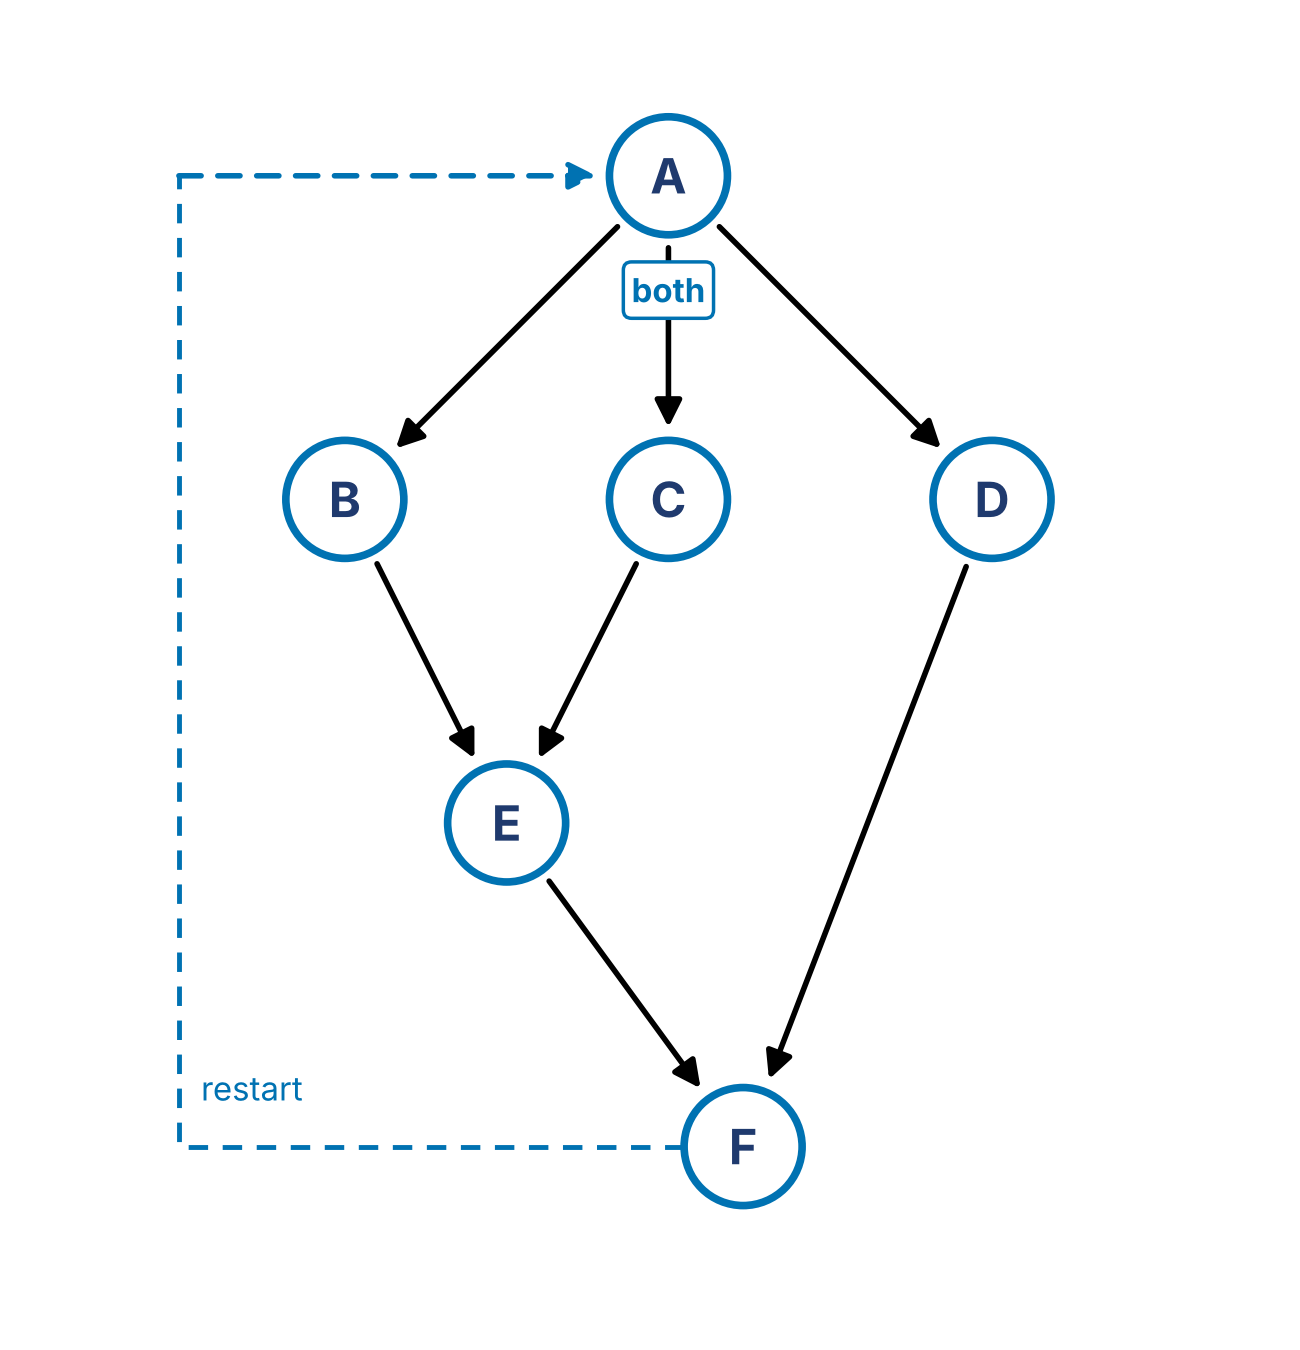
\includegraphics[width=0.4\textwidth]{contents/images/week-08/ex_add3.png}
\end{center}
\needspace{4\baselineskip}
\textbf{Solution.} Six semaphores, one per task, because every task runs in every round.
\begin{lstlisting}[basicstyle=\ttfamily\scriptsize]
semaphore sA = 1, sB = 0, sC = 0, sD = 0, sE = 0, sF = 0;

A: for ever: wait( sA );              CS A; signal( sB ); signal( sC ); signal( sD );
B: for ever: wait( sB );              CS B; signal( sE );
C: for ever: wait( sC );              CS C; signal( sE );
D: for ever: wait( sD );              CS D; signal( sF );
E: for ever: wait( sE ); wait( sE );  CS E; signal( sF );
F: for ever: wait( sF ); wait( sF );  CS F; signal( sA );
\end{lstlisting}
E waits for B and C. F waits for D and E, so it needs two tokens, not three: B and C reach F through E. \texttt{sE} and \texttt{sF} are counting, with a maximum of 2; \texttt{sA} starts at 1: \texttt{xSemaphoreCreateCounting( 1, 1 )}.

\paragraph{Add the semaphores (4).} Two first tasks: both must finish before C, and each round restarts both. The fork at C is exclusive. How many semaphores start at 1? Which must be counting in FreeRTOS?
\begin{center}
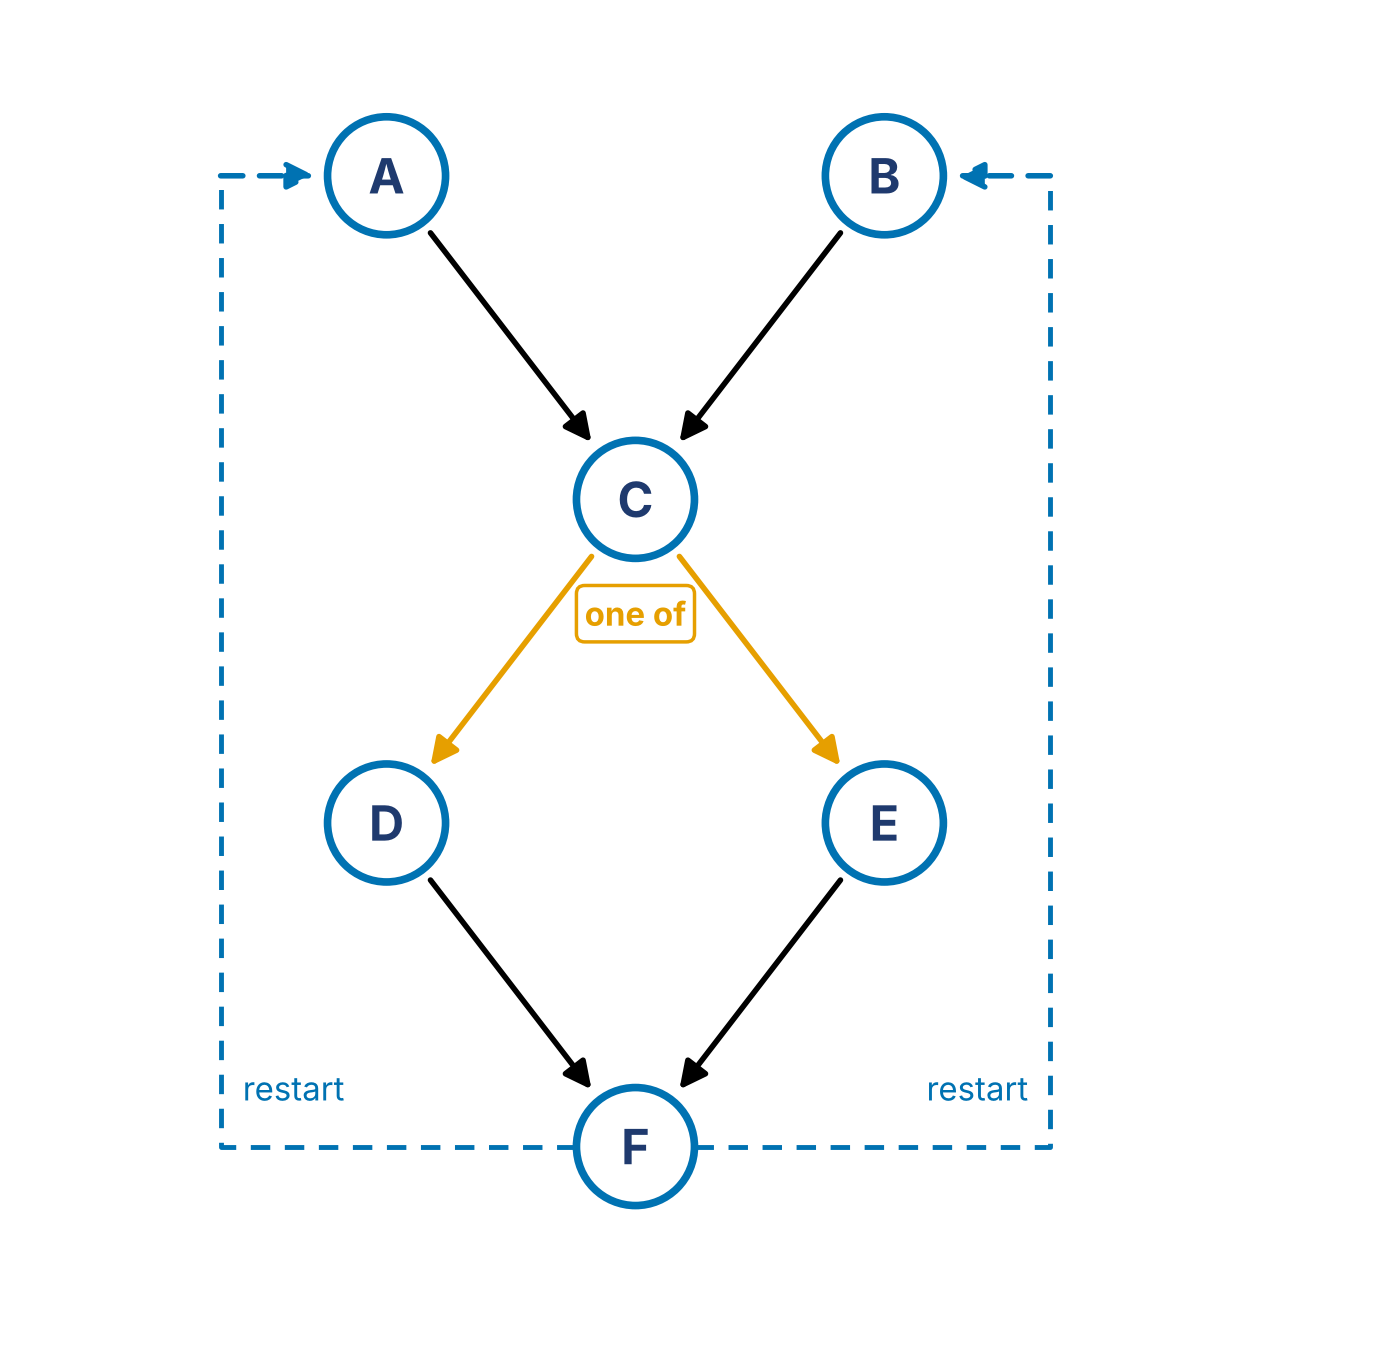
\includegraphics[width=0.42\textwidth]{contents/images/week-08/ex_add4.png}
\end{center}
\needspace{4\baselineskip}
\textbf{Solution.} Five semaphores: six tasks, with D and E counted as one.
\begin{lstlisting}[basicstyle=\ttfamily\scriptsize]
semaphore sA = 1, sB = 1, sC = 0, sX = 0, sF = 0;

A: for ever: wait( sA );              CS A; signal( sC );
B: for ever: wait( sB );              CS B; signal( sC );
C: for ever: wait( sC ); wait( sC );  CS C; signal( sX );
D: for ever: wait( sX );              CS D; signal( sF );
E: for ever: wait( sX );              CS E; signal( sF );
F: for ever: wait( sF );              CS F; signal( sA ); signal( sB );
\end{lstlisting}
\begin{itemize}
    \item Two semaphores start at 1, \texttt{sA} and \texttt{sB}: each first task needs its own token to begin the first round, and F gives both back.
    \item \texttt{sC} is counting, with a maximum of 2, because A and B may both finish first.
    \item C signals once and F waits once, because only one of D and E runs.
\end{itemize}
If you master precedence graphs, you can build basically any type of synchronization in your system.

\subsection{Classic problem: the bounded buffer}
Now realistic uses of semaphores, built completely. The first is \textbf{producer and consumer}, or \textbf{bounded buffer}, found all the time in embedded systems: a \textbf{shared buffer} (an array, a memory region), a task that writes into it and one that reads from it.
\begin{figure}[H]
    \centering
    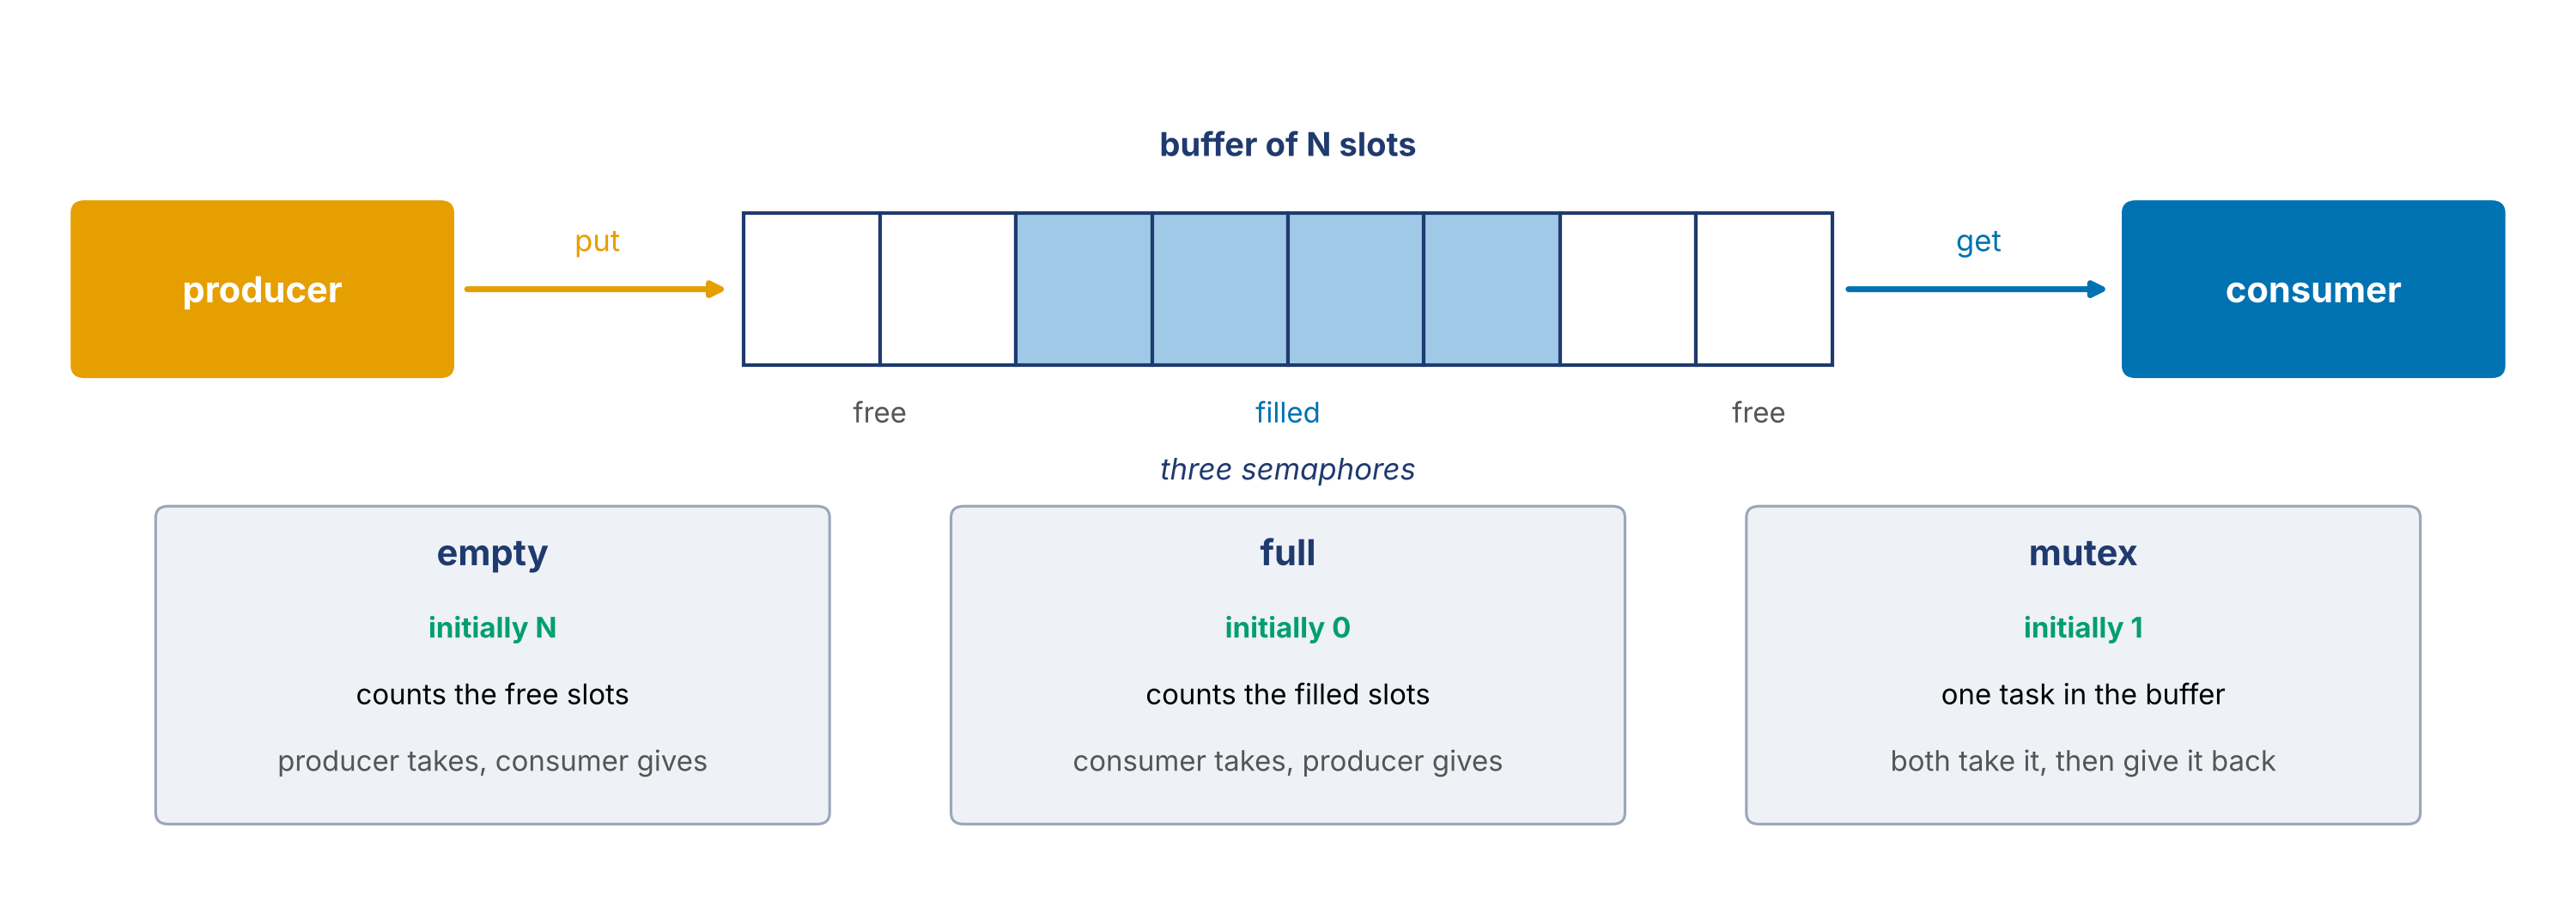
\includegraphics[width=1\textwidth]{contents/images/week-08/bounded_buffer.png}
    \caption{The bounded buffer: a producer puts items, a consumer gets them, through N slots; three semaphores coordinate them.}
\end{figure}
When the buffer is \textbf{full} the producer must wait; when it is \textbf{empty} the consumer must wait; only one task at a time may change it. Three needs, three semaphores, each starting at what is true at the start: \texttt{empty} $=$ N (free slots), \texttt{full} $=$ 0 (filled slots), \texttt{mutex} $=$ 1 (the buffer is free). The two counters are updated by both tasks, so they are \textbf{counting semaphores}, objects made to be shared. Even a shared vector used by two tasks needs \textbf{several} semaphores.
\par\noindent\begin{minipage}[t]{0.44\textwidth}
\begin{lstlisting}[basicstyle=\ttfamily\scriptsize]
semaphore empty = N;
semaphore full  = 0;
semaphore mutex = 1;

Producer:
  for ever:
    item = make();
    wait( empty );
    wait( mutex );
    buffer[ in ] = item;
    in = ( in + 1 ) % N;
    signal( mutex );
    signal( full );

Consumer:
  for ever:
    wait( full );
    wait( mutex );
    item = buffer[ out ];
    out = ( out + 1 ) % N;
    signal( mutex );
    signal( empty );
    use( item );
\end{lstlisting}
\end{minipage}\hfill
\begin{minipage}[t]{0.53\textwidth}
\begin{lstlisting}[language=C, showstringspaces=false, basicstyle=\ttfamily\scriptsize]
empty = xSemaphoreCreateCounting( N, N );
full  = xSemaphoreCreateCounting( N, 0 );
mutex = xSemaphoreCreateMutex();  /* starts free */

/* Producer */
for( ;; )
{
    item = make();
    xSemaphoreTake( empty, portMAX_DELAY );
    xSemaphoreTake( mutex, portMAX_DELAY );
    buffer[ in ] = item;
    in = ( in + 1 ) % N;
    xSemaphoreGive( mutex );
    xSemaphoreGive( full );
}

/* Consumer: the same, with full and empty
 * swapped, and out instead of in. */
\end{lstlisting}
\end{minipage}
\begin{itemize}
    \item \textbf{First barrier}: \texttt{wait( empty )} passes only if a free slot exists, and takes it.
    \item \textbf{Second barrier}: with two producers and enough free slots, both pass the first barrier, but they must write \textbf{one at a time}. What really needs \texttt{mutex} is the index: write \texttt{buffer[ in ]} and increment \texttt{in} as one atomic step (the increment is several instructions, week 7). The \texttt{\% N} makes the buffer \textbf{circular}.
    \item \texttt{signal( mutex )} lets the next one in; \texttt{signal( full )} adds a filled slot. \texttt{empty} and \texttt{full} count in \textbf{opposite} directions. The consumer is the mirror image.
    \item While a task works on a slot, that slot is in neither count, so \texttt{empty + full} can be less than N.
\end{itemize}
\emph{Why two counters, and not one?} (A question to the class.) With room and items, producer and consumer may run in parallel on different slots; at the two ends they must follow an \textbf{order}: with an empty buffer the consumer waits for the producer, with a full one the producer waits for the consumer (with one slot, it is the graph with the restart: producer, consumer, producer, \dots). One counter cannot make one side wait on ``no free slot'' and the other on ``no filled slot''. The code is short, but a very simple mistake destroys everything:

\paragraph{Try it on paper: the bounded buffer.}
\begin{enumerate}
    \item The producer swaps its two waits: \texttt{wait( mutex ); wait( empty );}. What can happen?
    \item The producer swaps its two signals: \texttt{signal( full ); signal( mutex );}. What can happen?
    \item With exactly one producer and one consumer, could you remove \texttt{mutex}? And with two producers?
    \item What does the solution become when N $=$ 1?
\end{enumerate}
\needspace{4\baselineskip}
\textbf{Solution.}
\begin{enumerate}
    \item \textbf{Both stop for ever.} With the buffer full, the producer holds \texttt{mutex} and sleeps on \texttt{empty}; the consumer needs \texttt{mutex} before it can free a slot, so it blocks, and nobody can give \texttt{empty} (figure below). A \textbf{deadlock} (Unit 3): the order of two \texttt{wait}s can matter a lot.
    \item \textbf{Nothing bad.} A signal never blocks. The consumer may wake a moment earlier, and then waits a moment on \texttt{mutex}.
    \item \textbf{One of each: yes.} \texttt{in} and \texttt{out} each belong to one task, and \texttt{empty} and \texttt{full} keep them away from the same slot. \textbf{Two producers: no.} They share \texttt{in}: the lost update of week 7.
    \item \texttt{empty} and \texttt{full} alternate between 0 and 1, so producer and consumer \textbf{take turns}: put, get, put, \dots
\end{enumerate}
\begin{figure}[H]
    \centering
    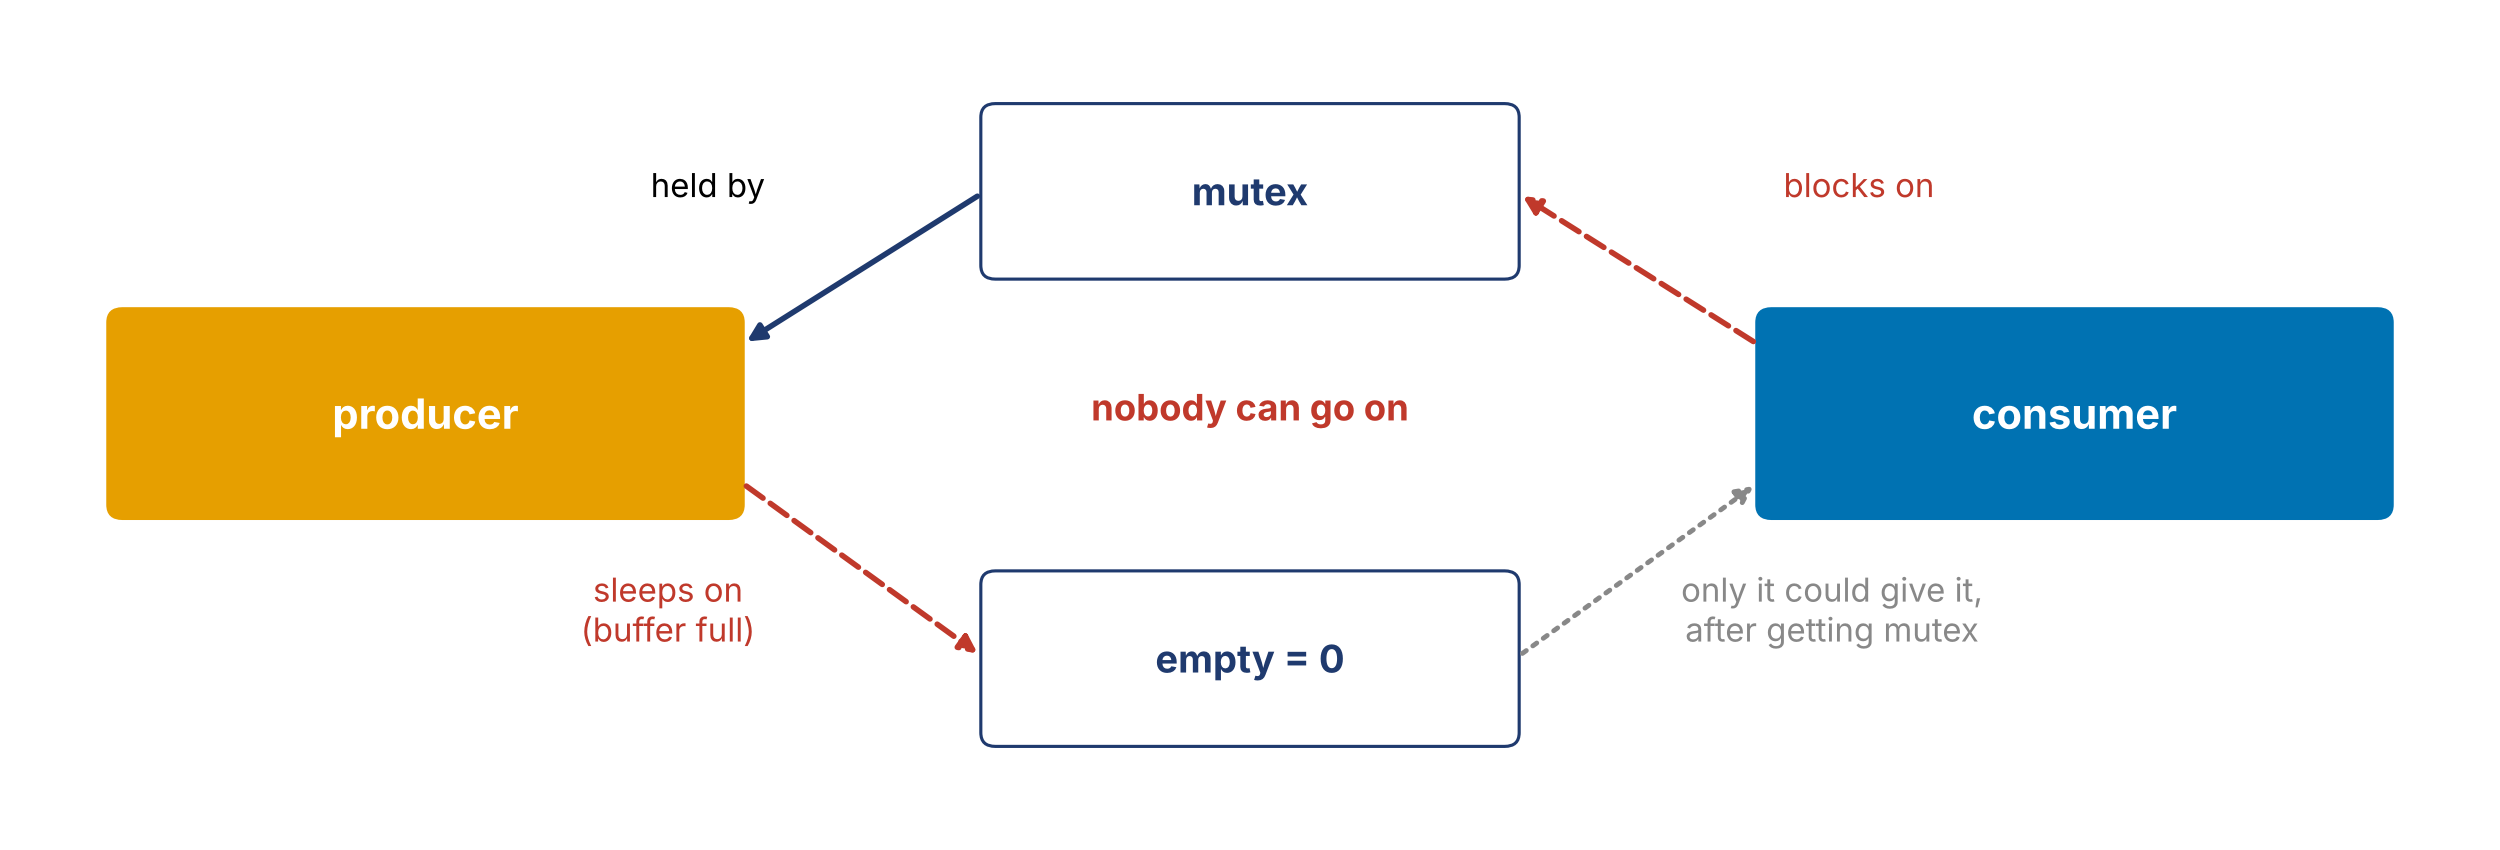
\includegraphics[width=0.72\textwidth]{contents/images/week-08/bb_swapped_waits.png}
    \caption{Answer 1: the producer holds \texttt{mutex} and sleeps on \texttt{empty}; the consumer, the only task that could give \texttt{empty}, blocks on \texttt{mutex}.}
\end{figure}

\subsection{Classic problem: readers and writers}
Many tasks share some data: \textbf{readers} only look at it, \textbf{writers} change it. Unlike the consumer, a reader removes nothing, so readers do no harm and can work \textbf{together}; a writer must be alone.
\begin{center}
\small
\begin{tabular}{l P{0.35} P{0.25}}
    \hline
    & \textbf{a reader is inside} & \textbf{a writer is inside} \\
    \hline
    a reader arrives & enters: reading together is harmless & waits \\
    a writer arrives & waits & waits \\
    \hline
\end{tabular}
\end{center}
A plain mutex is correct, but too strict: one reader at a time. The idea is a \textbf{room with one lock}, \texttt{rw}. A writer locks it for itself. Readers lock it \textbf{as a group}: the \textbf{first} reader in locks it, the \textbf{last} reader out unlocks it, those in between walk straight in. To know who is first and last, readers keep a count, \texttt{readers}, protected by \texttt{mutex}.
\par\noindent\begin{minipage}[t]{0.4\textwidth}
\begin{lstlisting}[basicstyle=\ttfamily\scriptsize]
semaphore rw = 1;    /* room lock */
semaphore mutex = 1; /* for readers */
int readers = 0;     /* inside now */

Writer:
  for ever:
    wait( rw );
    write the data;
    signal( rw );
\end{lstlisting}
\end{minipage}\hfill
\begin{minipage}[t]{0.58\textwidth}
\begin{lstlisting}[basicstyle=\ttfamily\scriptsize]
Reader:
  for ever:
    wait( mutex );
    readers = readers + 1;
    if ( readers == 1 ) wait( rw );   /* first in */
    signal( mutex );

    read the data;                    /* no lock */

    wait( mutex );
    readers = readers - 1;
    if ( readers == 0 ) signal( rw ); /* last out */
    signal( mutex );
\end{lstlisting}
\end{minipage}
\begin{itemize}
    \item \textbf{The writer} is a plain lock around its critical section: the first writer takes \texttt{rw} and enters.
    \item \textbf{The reader} increments the count; if it is the first, it waits on \texttt{rw}: it blocks if a writer is inside, otherwise it takes \texttt{rw} and keeps the writers out while the readers read. On leaving it decrements the count, and the last one gives \texttt{rw} back. \texttt{mutex} is held only to update and test the count, so it is free while reading.
\end{itemize}
\begin{figure}[H]
    \centering
    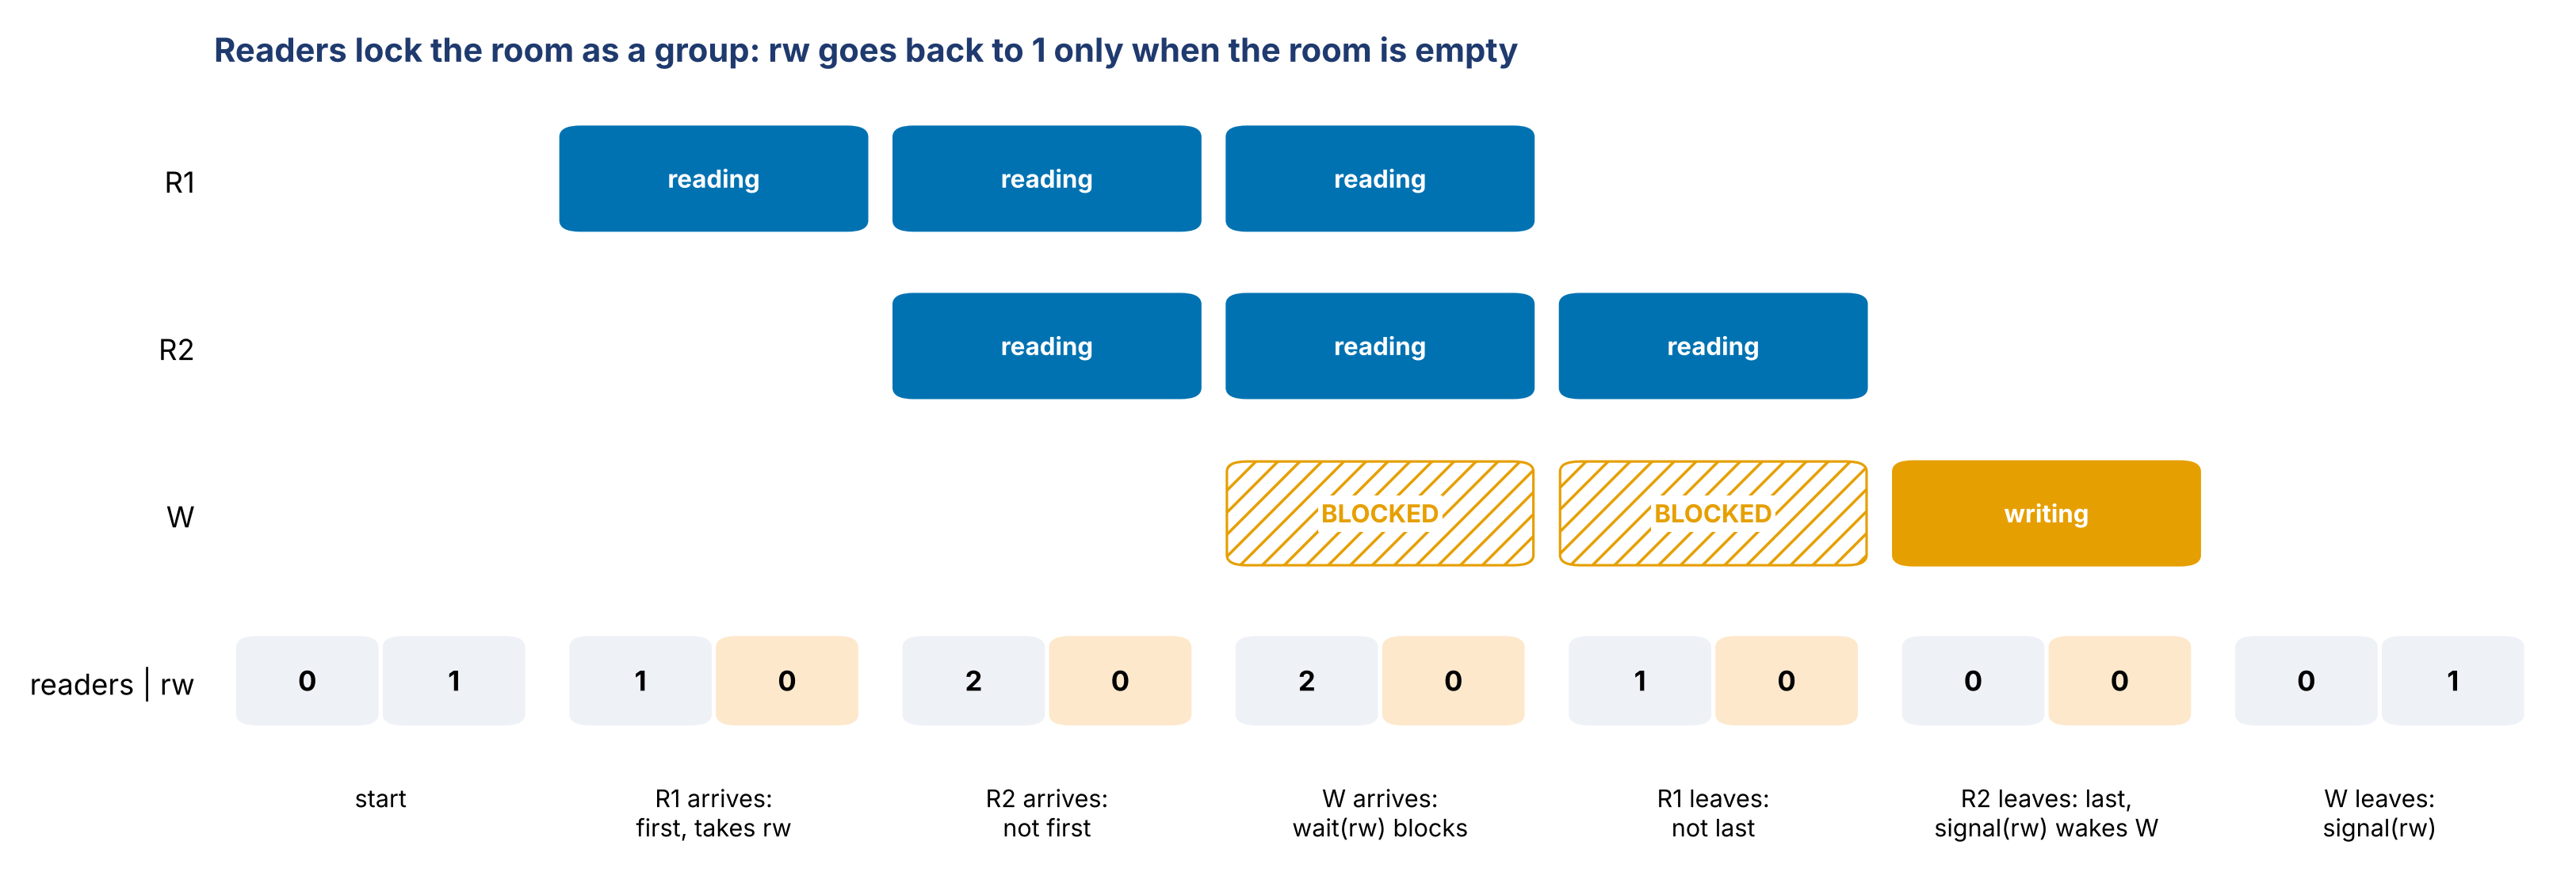
\includegraphics[width=1\textwidth]{contents/images/week-08/readers_writers.png}
    \caption{One run: R1 and R2 read together; W blocks on \texttt{rw}; only when the last reader leaves is \texttt{rw} given, and W writes. While any reader is inside, the group holds \texttt{rw}.}
\end{figure}

\paragraph{Why \texttt{mutex}?} \texttt{readers} is shared too, and the test depends on it. Remove \texttt{mutex}:
\begin{center}
\small
\begin{tabular}{l c c P{0.38}}
    \hline
    \textbf{step} & \texttt{readers} & \texttt{rw} & \textbf{what goes wrong} \\
    \hline
    R1: \texttt{readers = readers + 1} & 1 & 1 & \\
    R2: \texttt{readers = readers + 1} & 2 & 1 & R1 has not tested the count yet \\
    R1: \texttt{readers == 1}? No & 2 & 1 & R1 is the first, but does not know it \\
    R2: \texttt{readers == 1}? No & 2 & 1 & nobody took \texttt{rw} \\
    W: \texttt{wait( rw )} passes & 2 & 0 & W writes while R1 and R2 read \\
    \hline
\end{tabular}
\end{center}
The count and its test must be one atomic step. With \texttt{mutex}, listing all the runs of two readers and one writer finds no writer next to a reader, and no run that stops for ever.

\paragraph{Try it on paper: readers and writers.} A writer is inside. Then R1 and R2 arrive, in that order.
\begin{enumerate}
    \item Where does each reader wait?
    \item In FreeRTOS, can \texttt{rw} be a mutex (\texttt{xSemaphoreCreateMutex})?
    \item A reader is inside, a writer is waiting, and new readers keep arriving. Who goes first?
\end{enumerate}
\needspace{4\baselineskip}
\textbf{Solution.}
\begin{enumerate}
    \item R1 waits on \texttt{rw}, \textbf{holding} \texttt{mutex}. R2 waits on \texttt{mutex}. When the writer signals \texttt{rw}, R1 goes on and gives \texttt{mutex}, then R2 enters without touching \texttt{rw}.
    \item \textbf{No.} A mutex has an owner, and only the owner may release it; here the first reader takes \texttt{rw} and the last one gives it, possibly another task. Use \texttt{xSemaphoreCreateCounting( 1, 1 )}\footnote{In class the writer's lock was ``a binary semaphore initialised to 1'': right on paper, but a FreeRTOS binary semaphore starts at 0, and a mutex is wrong for the reason above.}.
    \item \textbf{The new readers.} They find \texttt{readers} above 0 and walk straight in. As long as readers overlap, \texttt{rw} is never given, and the writer \textbf{starves}: bounded waiting (week 7) fails. This solution is unfair to writers; fairer versions need more semaphores.
\end{enumerate}

\paragraph{Why these two examples?} They are two \textbf{common design patterns} of FreeRTOS applications: sharing between a producer and a consumer, or between many readers and writers. They come back in the \textbf{second part of the exam}, where you write an application. The slides and the exercise files have many more exercises: \textbf{they are really exam exercises}, so solve them all on paper.

\section{Unit 1: summary}
\begin{itemize}
    \item \textbf{Notation}: \texttt{wait}/\texttt{signal} on paper, \texttt{xSemaphoreTake}/\texttt{xSemaphoreGive} in FreeRTOS. A FreeRTOS semaphore has a maximum (a give on a full one loses the token); a binary semaphore always starts at 0, so a semaphore that starts at 1 is \texttt{xSemaphoreCreateCounting( 1, 1 )}. Every take has a timeout: \texttt{portMAX\_DELAY} waits for ever.
    \item \textbf{Precedence graphs} with cyclic tasks: one round per graph, a dashed restart, joins and forks. A fork is \textbf{concurrent} (``both'', \texttt{\&}: every branch runs in every round) or \textbf{exclusive} (``one of'', \texttt{|}: exactly one branch runs); the exercise must say which. Read a graph by its edges, not by layers.
    \item \textbf{The method}: one semaphore per edge, at 0, plus the restart at 1; each task waits once per incoming edge and signals once per outgoing edge. Always correct, and the first thing to write at the exam.
    \item \textbf{Fewer semaphores}: a token has no name, and the loop comes back. Two tasks that must both run in a round never wait on the same semaphore (or one steals the other's token). Sharing at a \textbf{join} is safe; at a concurrent fork it is wrong; the branches of an \textbf{exclusive} fork share one semaphore, signalled once. The minimum is one semaphore per task, with the branches of an exclusive fork counted as one; a join waits once per branch that runs, and the maximum of a counting semaphore is its number of incoming edges.
    \item \textbf{Bounded buffer}: \texttt{empty} (N), \texttt{full} (0), \texttt{mutex} (1); swapping the two waits gives a deadlock, swapping the signals is harmless.
    \item \textbf{Readers and writers}: a writer locks \texttt{rw}; readers lock it as a group, the first in and the last out, with the count protected by \texttt{mutex}. \texttt{rw} cannot be a FreeRTOS mutex (no single owner), and the writers can starve.
\end{itemize}

\section{Unit 2 - Blocking primitives in FreeRTOS}
After the break, code in FreeRTOS: first the primitives that implement synchronization in practice, then the programs. In this unit file paths are relative to \texttt{week-08/\allowbreak solution/}, kernel files are written from \texttt{FreeRTOS/Source/}, and commands run in \texttt{week-08/base/} (to write the code) or in the solution folder (to see it run).

\subsection{Four mechanisms, and how to choose}
A \textbf{blocking primitive} is an object that a task can wait on, BLOCKED and using no CPU. FreeRTOS has four in common use (the others are variations of these). The theory's concepts are kept, and used to solve realistic problems.
\begin{figure}[H]
    \centering
    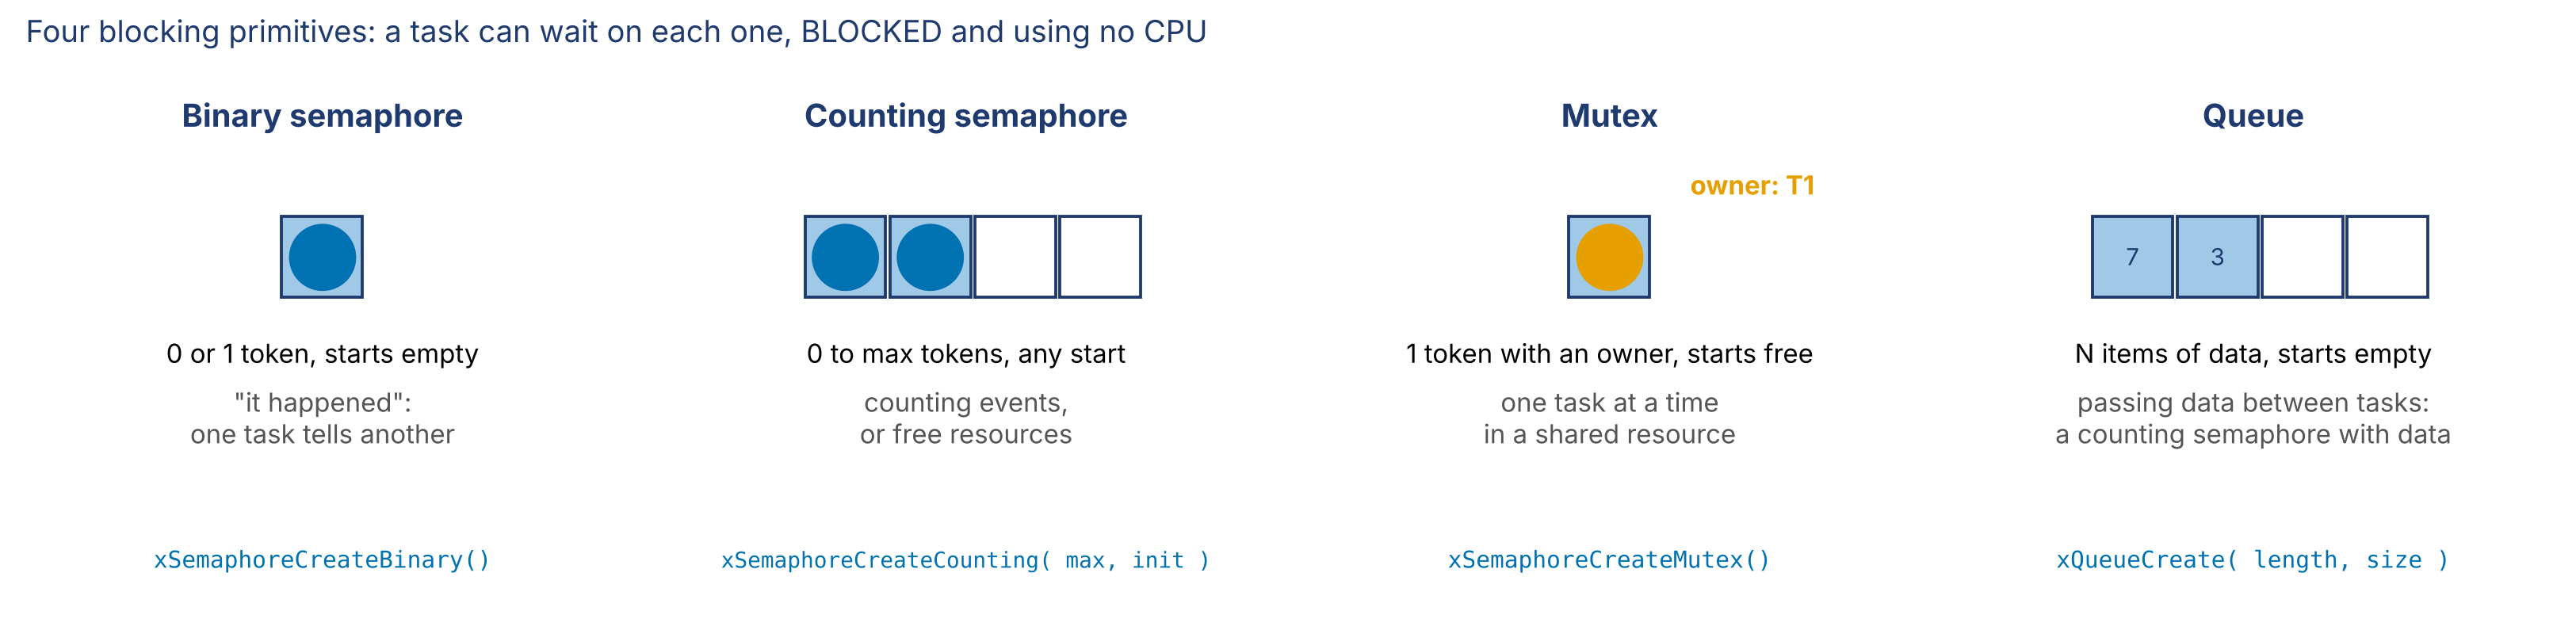
\includegraphics[width=1\textwidth]{contents/images/week-08/four_mechanisms.png}
    \caption{The four blocking primitives, with the function that creates each one. The three semaphores carry no data and use \texttt{xSemaphoreTake} and \texttt{xSemaphoreGive}; the queue uses \texttt{xQueueSend} and \texttt{xQueueReceive}.}
\end{figure}
\begin{itemize}
    \item \textbf{Binary and counting semaphores} are the theoretical semaphore, one to one. Two objects because their complexity differs, and a binary semaphore must never count above 1.
    \item \textbf{The mutex} is, in theory, a binary semaphore with an \textbf{owner}. A semaphore does not remember who signalled: a binary semaphore locked by a task can be unlocked by \textbf{any} task; a mutex only by the task that locked it.
    \item \textbf{The queue} works like a counting semaphore whose tokens carry a \textbf{data structure}: a send is a signal with data attached, a receive is a wait that gets the content.
    \item \emph{Why do these names start with \texttt{x}?} (A question to the class.) The prefix tells the return type: \texttt{x} returns a value (here the new object), \texttt{v} returns nothing (week 7).
\end{itemize}
\paragraph{Choosing a mechanism.} Any problem can be solved with semaphores alone; in practice, start from the requirement and pick the right object. The last column names this week's program where the case appears, as a template:
\begin{center}
\small
\begin{tabular}{P{0.45} P{0.3} P{0.15}}
    \hline
    \textbf{we want} & \textbf{use} & \textbf{we write it in} \\
    \hline
    Y starts only after X has finished & binary semaphore & \texttt{precedence} \\
    Z waits for two tasks, whose tokens may both arrive first & counting semaphore & \texttt{precedence} \\
    a fast task and a slow task pass data through a buffer & queue & \texttt{prodcons} \\
    only one task uses a shared device, with no lock & queue, and one task that owns the device & \texttt{gatekeeper} \\
    only one task at a time changes shared data & mutex & \texttt{deadlock} \\
    \hline
\end{tabular}
\end{center}
\begin{itemize}
    \item \textbf{Producer and consumer}: our solution needed three semaphores; FreeRTOS made the common problem \textbf{one object}. No circular buffer to get right: use a queue.
    \item \textbf{Gatekeeper}: instead of synchronizing on a shared device (our UART), give it to \textbf{one task}, the only one that writes to it, and let the others pass their data through a queue. Printing is very slow, so in the professor's view the printing task can even have a \textbf{very low} priority, almost like the idle task (the program here gives it a higher one, and discusses both).
    \item \textbf{Mutual exclusion}: the \textbf{mutex}, so the shared resource gets a named owner.
\end{itemize}

\subsection{Semaphores, mutexes and queues in FreeRTOS}
\begin{lstlisting}[language=C, showstringspaces=false, basicstyle=\ttfamily\scriptsize]
SemaphoreHandle_t s;                           /* the handle, from "semphr.h" */

s = xSemaphoreCreateBinary();                  /* holds 0 or 1, starts at 0 (empty) */
s = xSemaphoreCreateCounting( max, initial );  /* holds 0 to max, starts at initial */
s = xSemaphoreCreateMutex();                   /* lock with an owner, starts free */

xSemaphoreTake( s, timeout );                  /* wait( s ) */
xSemaphoreGive( s );                           /* signal( s ) */
uxSemaphoreGetCount( s );                      /* reads the count; for a look only */
\end{lstlisting}
\begin{itemize}
    \item Header \texttt{semphr.h}\footnote{In class it was called ``semaphore.h''; the FreeRTOS header is \texttt{semphr.h}.}; one type, \texttt{SemaphoreHandle\_t}, for all three. A \textbf{handle} names a kernel object in later calls: you never look inside it.
    \item Binary and mutex are created with no argument, counting with the maximum and the initial value. \texttt{uxSemaphoreGetCount} is ``for a look only'': the count can change right after you read it, so print it, never use it to decide that a take will not block.
    \item \textbf{A binary semaphore and a mutex differ from the first take.} The binary starts \textbf{empty}, so the take blocks until someone gives: use it to \textbf{signal}. The mutex starts \textbf{free}, so the take succeeds and the caller becomes the owner: use it to \textbf{protect shared data}.
    \item The same take and give serve all three; the behaviour differs. A binary semaphore given many times stays at 1. A mutex given by a task that is not its owner: in class, ``the give will not do anything''; in our configuration (\texttt{configASSERT} on) the program \textbf{stops with an assertion failure}, because the give path checks that the owner is the current task.
\end{itemize}
\paragraph{Queues.} A kernel object that holds a fixed number of items of a fixed size, first in first out, to pass data. It has its own type, as a different data structure.
\begin{lstlisting}[language=C, showstringspaces=false, basicstyle=\ttfamily\scriptsize]
QueueHandle_t q;                             /* the handle, from "queue.h" */

q = xQueueCreate( length, sizeof( item ) );  /* room for length items */

xQueueSend( q, &item, timeout );             /* copies item in, at the back */
xQueueReceive( q, &item, timeout );          /* copies the oldest item out */
uxQueueSpacesAvailable( q );                 /* how many free places now */
\end{lstlisting}
\begin{itemize}
    \item \emph{Why both the length and the item size?} (A question to the class.) To \textbf{allocate the memory}: somewhere there is a \texttt{malloc} of length $\times$ item size.
    \item \texttt{xQueueSend} blocks when the queue is \textbf{full}, \texttt{xQueueReceive} when it is \textbf{empty}, each for at most its timeout. \texttt{uxQueueSpacesAvailable} only looks.
    \item Items are \textbf{copied}: after the send the sender can reuse its variable. So never send a pointer to a local variable: the queue copies the pointer, not the data, which may be gone when the receiver looks.
\end{itemize}

\subsection{The event-driven task}
Last week's template was the \textbf{periodic} task: work, wait for the rest of the period, again. Often a task has work only when something \textbf{happens}: another task finished, data arrived. An \textbf{event} is any such happening. The \textbf{event-driven} task (the \textbf{aperiodic} model of week 5) is still an infinite loop, but at each iteration it \textbf{stops and waits} for its event:
\begin{lstlisting}[language=C, showstringspaces=false, basicstyle=\ttfamily\footnotesize]
static void vHandler( void * pvParameters )
{
    ( void ) pvParameters;

    for( ;; )
    {
        xSemaphoreTake( xEvent, portMAX_DELAY );  /* BLOCKED until the event */
        /* handle the event */
    }
}
\end{lstlisting}
It does not test a flag in a loop, so it uses \textbf{no CPU} while it waits. The wait can be \texttt{xSemaphoreTake} or \texttt{xQueueReceive}, and with a queue the event also brings data.
\begin{figure}[H]
    \centering
    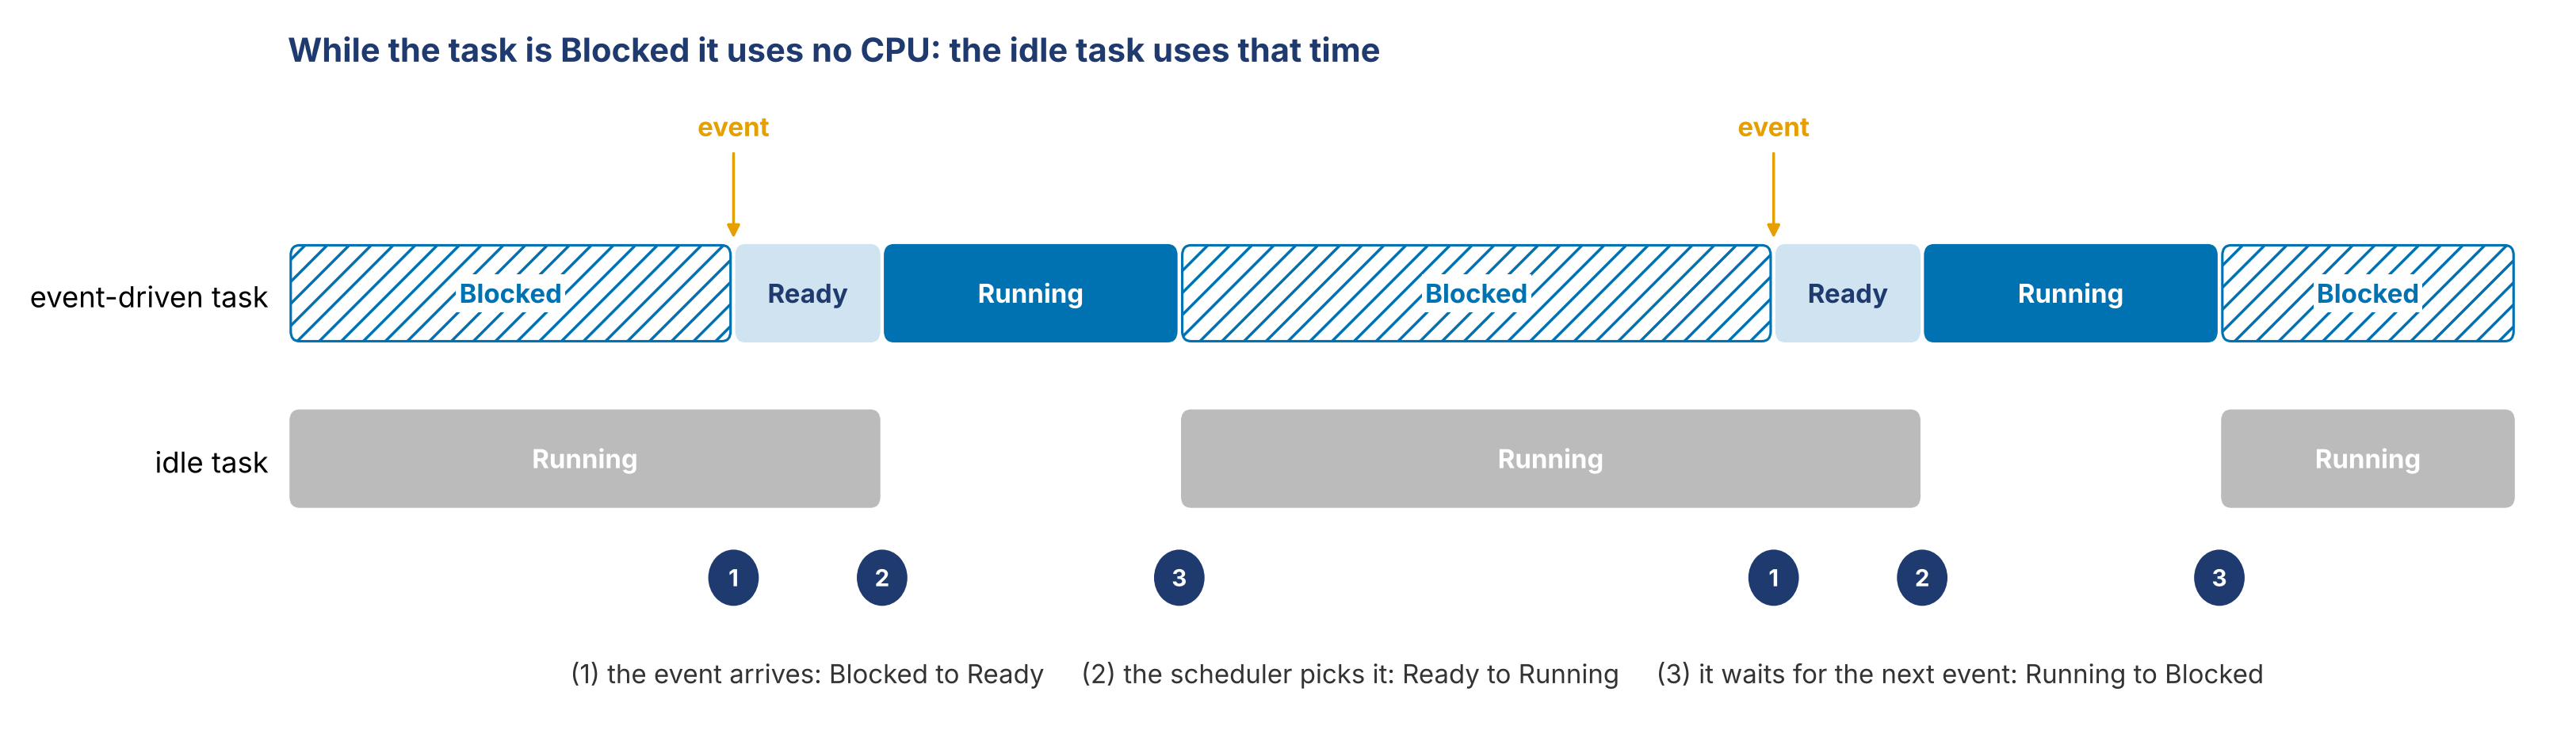
\includegraphics[width=1\textwidth]{contents/images/week-08/event_task.png}
    \caption{An event-driven task, and the idle task that uses the CPU while it is Blocked.}
\end{figure}
\begin{enumerate}
    \item \textbf{BLOCKED $\rightarrow$ READY}: the event happens, for example another task calls \texttt{xSemaphoreGive}. Until then the task uses no CPU: if nothing else is READY, the idle task runs.
    \item \textbf{READY $\rightarrow$ RUNNING}: the scheduler picks the highest-priority READY task; if it is this one, it runs \textbf{at once}\footnote{In class: with a poorly optimised round robin, the idle task might keep the CPU until the end of its quantum. FreeRTOS with preemption, as configured here, switches at once to a woken task of higher priority than the running one.}.
    \item \textbf{RUNNING $\rightarrow$ BLOCKED}: the handler has finished and calls the wait again.
\end{enumerate}

\subsection{Blocking calls: timeouts and return codes}
Every call that can block takes a \textbf{timeout}, in ticks: how long the task accepts to wait if the object is not ready.
\begin{figure}[H]
    \centering
    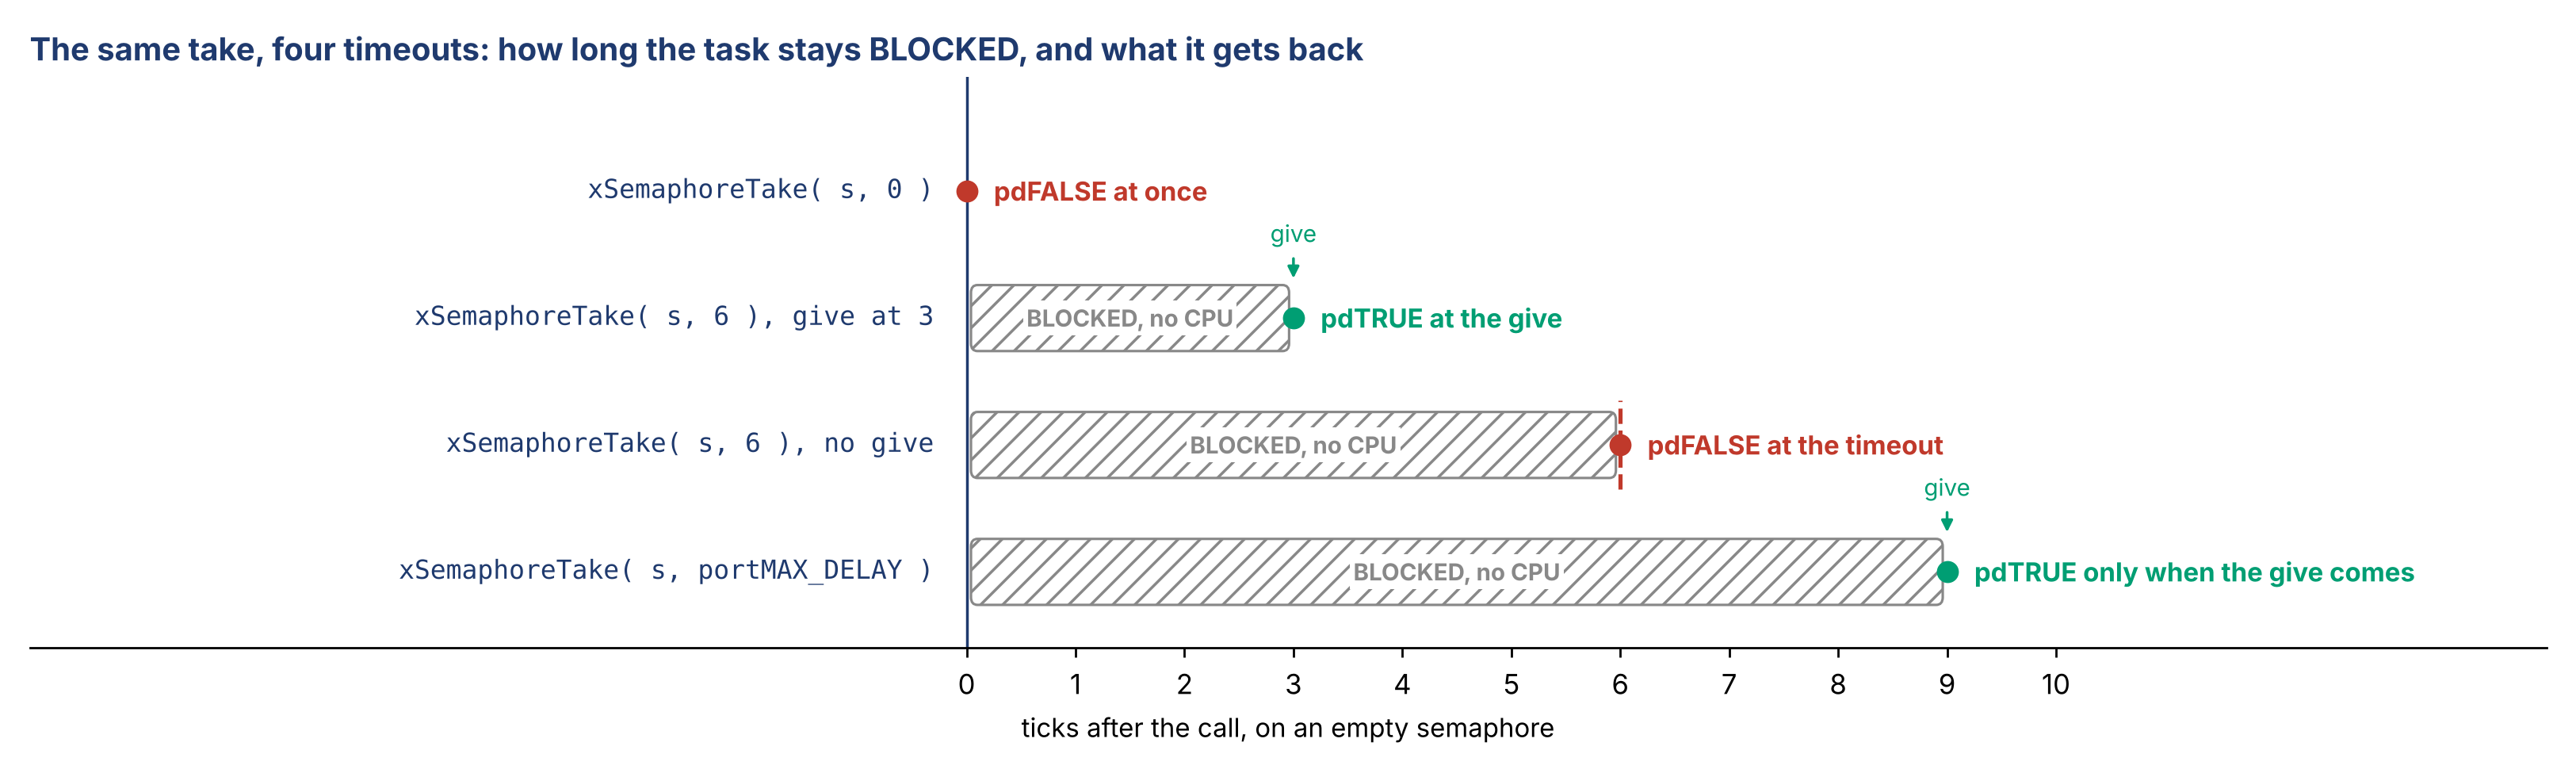
\includegraphics[width=1\textwidth]{contents/images/week-08/timeouts.png}
    \caption{The same take on an empty semaphore with four timeouts. While it waits the task is BLOCKED and uses no CPU; with a finite timeout it can come back with either result, so the return code must be tested.}
\end{figure}
\begin{center}
\small
\begin{tabular}{P{0.35} P{0.5}}
    \hline
    \textbf{timeout value} & \textbf{if the object is not ready} \\
    \hline
    \texttt{0} & returns at once with a failure code \\
    \texttt{pdMS\_TO\_TICKS( 300 )}, or N ticks & BLOCKED for at most that time, then returns a failure code \\
    \texttt{portMAX\_DELAY} & BLOCKED as long as it takes (needs \texttt{INCLUDE\_vTaskSuspend}, set to 1 in our config) \\
    \hline
\end{tabular}
\end{center}
A timeout of 0 means ``I do not want to wait''. Other values are in \textbf{ticks}, and \texttt{pdMS\_TO\_TICKS} converts from milliseconds, because \texttt{FreeRTOSConfig.h} sets the tick length. (``As always, what I remembered was wrong'': the guess on \texttt{portMAX\_DELAY} in the first part is why you keep the documentation open.) With a finite timeout the call may fail, so the code has two branches:
\begin{lstlisting}[language=C, showstringspaces=false, basicstyle=\ttfamily\footnotesize]
if( xSemaphoreTake( xLock, pdMS_TO_TICKS( 300 ) ) == pdTRUE )
{
    /* taken: use the resource, then give it back */
}
else
{
    /* NOT taken: do something else, and do NOT give */
}
\end{lstlisting}
\textbf{Rule}: with a finite timeout, always check the return code. After a failure you hold nothing, and how to handle it depends on the application.
\begin{center}
\small
\begin{tabular}{l l l P{0.3}}
    \hline
    \textbf{call} & \textbf{success} & \textbf{failure} & \textbf{failure means} \\
    \hline
    \texttt{xSemaphoreTake} & \texttt{pdTRUE} & \texttt{pdFALSE} & no token within the timeout \\
    \texttt{xSemaphoreGive} & \texttt{pdTRUE} & \texttt{pdFALSE} & the semaphore is full (a give never waits) \\
    \texttt{xQueueSend} & \texttt{pdPASS} & \texttt{errQUEUE\_FULL} & no free place within the timeout \\
    \texttt{xQueueReceive} & \texttt{pdPASS} & \texttt{errQUEUE\_EMPTY} & no item within the timeout \\
    \hline
\end{tabular}
\end{center}
\texttt{pdPASS} equals \texttt{pdTRUE}, and the failure codes are all 0. With \texttt{portMAX\_DELAY} a take, send or receive returns only on success, so our programs do not test it. A task that calls \texttt{xQueueSend( q, \&m, 0 )} on a full queue gets \texttt{errQUEUE\_FULL} at once: the queue does not have \texttt{m}, the variable still holds it, and the task decides whether to retry later or drop it.

\paragraph{Documentation at the exam.} This table, and every function, is in the documentation: keep it with you whenever you write FreeRTOS code. At the written exam the \textbf{FreeRTOS website} is accessible, so when you do not remember a function, search for it.

\subsection{The week-08 folder}
Four programs, one file each:
{\verbatimscriptsize
\begin{verbatim}
apps/precedence.c   cyclic A, B, C, D of Example 1 (DEMO=steal: wrong, DEMO=xor: exclusive fork)
apps/prodcons.c     bounded buffer of 4 with a queue (DEMO=sem: semaphores)
apps/gatekeeper.c   only one task writes to the UART
apps/deadlock.c     two mutexes, a monitor task (DEMO=ordered, DEMO=timeout)
bsp/trace.c         new, given: records every task switch, prints it on request
\end{verbatim}}
\begin{lstlisting}[language=bash]
    cd week-08/base
    make APP=precedence run                  # build and run one program
    make APP=precedence DEMO=xor run         # build it with one variant
\end{lstlisting}
\begin{itemize}
    \item \texttt{APP} chooses the program, \texttt{DEMO} one deliberate change: \texttt{steal}, \texttt{xor}, \texttt{sem}, \texttt{ordered}, \texttt{timeout} (any other word stops the build with a clear message). \texttt{DEMO=xor} defines \texttt{DEMO\_XOR}, and the C code selects its version with \texttt{\#ifndef DEMO\_XOR}. Quit QEMU with \texttt{Ctrl-C}: the programs never exit.
    \item \texttt{FreeRTOSConfig.h} has four new settings: \texttt{configUSE\_COUNTING\_SEMAPHORES}; \texttt{configUSE\_TRACE\_FACILITY} with \texttt{configUSE\_STATS\_FORMATTING\_FUNCTIONS}, for \texttt{vTaskList}; \texttt{INCLUDE\_xSemaphoreGetMutexHolder}. The last two are used in Unit 3.
    \item \textbf{The base} builds and boots, and each program prints only its banner: \texttt{main()} creates the tasks and starts the scheduler, and each task only \textbf{suspends} itself. The build, configuration, board support (UART functions in \texttt{bsp/}) and trace module are ready; you fill in the task bodies, the handles and their creation, each at a \textbf{marker comment}. Parts that are not the point of the exercise are given: \texttt{busy\_work}, \texttt{round\_done} and task R in \texttt{precedence}; the message type and sender descriptions in \texttt{gatekeeper}; the counters and \texttt{print\_task\_table} in \texttt{deadlock}.
    \item \textbf{The solution} is the finished code, commented line by line. \textbf{The kernel} is last week's, and you never edit it. Your code need not have the solution's shape, so these notes point to code by the \textbf{name} of a function or variable, never by its position.
\end{itemize}

\subsection{Try it: tasks that follow a graph}
\textbf{Requirement}: four cyclic tasks follow Example 1 of Unit 1, concurrent: A, then B and C, then D, and again. Given in \texttt{apps/precedence.c}:
\begin{itemize}
    \item \texttt{busy\_work( n )} keeps the CPU busy for n ticks \textbf{without blocking} (it reads the tick count in a loop), so a critical section really uses the CPU and shows in the trace; \texttt{JOB\_A} \dots\ \texttt{JOB\_D} are 2, 3, 2 and 2 ticks.
    \item \texttt{round\_done()}: D calls it at the end of each round; after 3 rounds it gives \texttt{sDone}, which is \textbf{not} an edge of the graph. Task R sleeps on it, then calls \texttt{trace\_dump} and keeps the CPU in an empty loop, so the output stays quiet.
    \item \textbf{The priorities} are on purpose the opposite of the order we want: A 1 (the lowest), B 2, C 3, D 4 (R also 4, but it sleeps). Without semaphores D would run first.
\end{itemize}

\paragraph{Where are the semaphores defined?} In \texttt{apps/precedence.c}, outside every function:
\begin{lstlisting}[language=C, showstringspaces=false, basicstyle=\ttfamily\footnotesize]
static SemaphoreHandle_t sA;
static SemaphoreHandle_t sB;
static SemaphoreHandle_t sC;
static SemaphoreHandle_t sD;
\end{lstlisting}
\begin{itemize}
    \item \emph{Why global, and not inside \texttt{main}?} (``Finally, after eight weeks, I can see you using your brain.'') They are \textbf{shared objects}. What is defined inside a function lives on a \textbf{stack}, and every task has its own; a global lives in \texttt{.bss} or \texttt{.data}, where every task sees it.
    \item \emph{Why \texttt{static}?} It limits the \textbf{visibility} to this file: a project has many files and libraries, and a global with the same name elsewhere would conflict.
\end{itemize}

\paragraph{Where are they created?} In \texttt{main}, before the scheduler starts:
\begin{lstlisting}[language=C, showstringspaces=false, basicstyle=\ttfamily\footnotesize]
sA = xSemaphoreCreateCounting( 1, 1 );  /* the restart token: A goes first */
sB = xSemaphoreCreateBinary();
sC = xSemaphoreCreateBinary();
sD = xSemaphoreCreateCounting( 2, 0 );  /* D waits for two tokens */
\end{lstlisting}
\begin{itemize}
    \item \emph{Why in \texttt{main}?} It depends on \textbf{when the tasks start}. Creating the semaphore between A and B inside both A and B (``never trust your professor'') makes two different objects: the first task creates it and uses it, then the other creates it again and the first value is forgotten. Create it \textbf{once}. In \textbf{this} example the only safe place is \texttt{main}; it is not a general rule.
    \item \textbf{The types} come from the paper solution. The professor first said ``binary, initialised to 1'' for \texttt{sA}, then looked at the code: counting, because a binary semaphore starts at 0 (a binary semaphore plus one give in \texttt{main} would work too). At the exam, a counting semaphore where a binary was enough is not penalised (``with 350 students I cannot go so deep'').
\end{itemize}

\paragraph{The tasks.} Wait, work, print, signal:
\par\noindent\begin{minipage}[t]{0.49\textwidth}
\begin{lstlisting}[language=C, showstringspaces=false, basicstyle=\ttfamily\scriptsize]
/* vTaskA: take the restart token,
 * work, enable both B and C */
for( ;; )
{
    xSemaphoreTake( sA, portMAX_DELAY );
    busy_work( JOB_A );
    console_print( "A: tick %lu\n",
        ( unsigned long ) xTaskGetTickCount() );
    xSemaphoreGive( sB );
    xSemaphoreGive( sC );
}

/* vTaskB: wait for A, tell D */
for( ;; )
{
    xSemaphoreTake( sB, portMAX_DELAY );
    busy_work( JOB_B );
    console_print( "B: tick %lu\n",
        ( unsigned long ) xTaskGetTickCount() );
    xSemaphoreGive( sD );
}
\end{lstlisting}
\end{minipage}\hfill
\begin{minipage}[t]{0.49\textwidth}
\begin{lstlisting}[language=C, showstringspaces=false, basicstyle=\ttfamily\scriptsize]
/* vTaskC: the same as B, on sC */
for( ;; )
{
    xSemaphoreTake( sC, portMAX_DELAY );
    busy_work( JOB_C );
    console_print( "C: tick %lu\n",
        ( unsigned long ) xTaskGetTickCount() );
    xSemaphoreGive( sD );
}

/* vTaskD: wait for both B and C,
 * then restart the round */
for( ;; )
{
    xSemaphoreTake( sD, portMAX_DELAY );
    xSemaphoreTake( sD, portMAX_DELAY );
    busy_work( JOB_D );
    console_print( "D: tick %lu\n",
        ( unsigned long ) xTaskGetTickCount() );
    round_done();
    xSemaphoreGive( sA );
}
\end{lstlisting}
\end{minipage}
\begin{itemize}
    \item \emph{Can A's two gives be swapped?} (A poll: two thirds said no, which is \textbf{wrong}.) Yes: both tasks are enabled whatever the order.
    \item Only the \textbf{sequence of takes and gives} matters; the busy work and the print are just examples, and whatever the durations, the order is the one of the semaphores.
    \item Only A, B, C, D are synchronized; other tasks (R) run in competition, by priority. A real application synchronizes a subset of its tasks, but with correct code you never see, for example, D before A.
    \item \emph{Why did the empty tasks of the base have \texttt{vTaskSuspend( NULL )}?} A FreeRTOS task function must \textbf{never return}: ``game over''\footnote{In class: a hard fault. In this port the return address of every task is \texttt{prvTaskExitError} (week 7), which stops the program with an assertion; either way nothing runs any more.}. With the infinite loop that line could go; a task with a complex flow that must end has to be \textbf{suspended} or stopped in another way.
\end{itemize}

\paragraph{Run it.} \texttt{make APP=precedence run | tee out.txt}, \texttt{Ctrl-C} after \texttt{TRACE END}, then\\ \texttt{python3 ../../../course-material/tools/schedsim/schedsim.py trace out.txt}.
\begin{figure}[H]
    \centering
    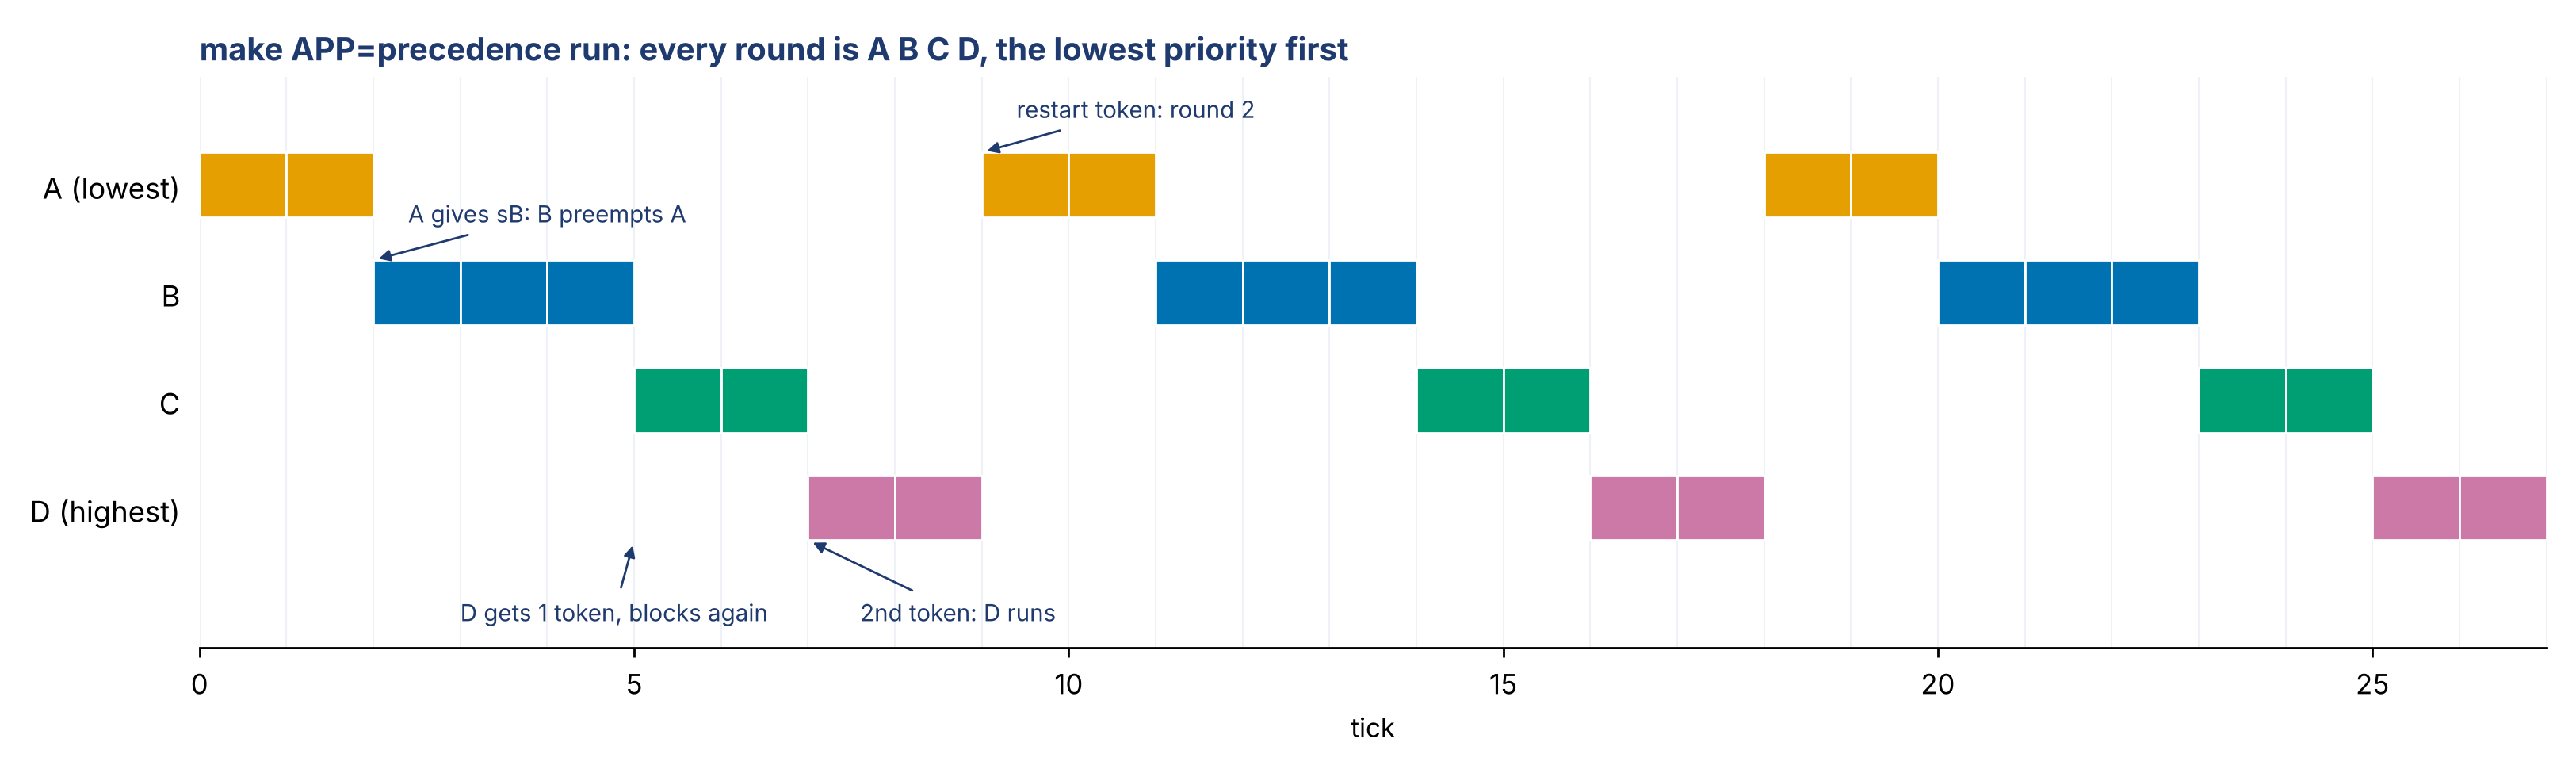
\includegraphics[width=1\textwidth]{contents/images/week-08/precedence_trace.png}
    \caption{The \texttt{schedsim} chart of the run, redrawn: the CPU line is \texttt{AABBBCCDDAABBBCCDD\dots}. \textbf{The graph wins}: every round is A B C D, the lowest priority first. The semaphores decide what is allowed, whatever the priorities say.}
\end{figure}
\paragraph{Reading the trace.} The program prints its lines, then the trace; a line \texttt{T <tick> <from> <to>} is one task switch.
\par\noindent\begin{minipage}[t]{0.25\textwidth}
{\verbatimscriptsize
\begin{verbatim}
A: tick 2
B: tick 5
C: tick 7
D: tick 9
...
TRACE BEGIN
T 0 idle R
T 0 R D
T 0 D C
T 0 C B
T 0 B A
T 2 A B
T 5 B D
T 5 D B
T 5 B A
T 5 A C
T 7 C D
T 9 D C
T 9 C A
...
\end{verbatim}}
\end{minipage}\hfill
\begin{minipage}[t]{0.72\textwidth}
\begin{itemize}
    \item \textbf{Tick 0}: R, D, C and B run in priority order, and each blocks at once on its semaphore (no CPU time, so all at the same tick). Only A goes on: it takes the restart token.
    \item \textbf{\texttt{T 2 A B}}: A gives \texttt{sB}, and B, of higher priority, preempts it \textbf{inside} \texttt{xSemaphoreGive}: A has not yet given \texttt{sC}.
    \item \textbf{\texttt{T 5 B D}, \texttt{D B}}: B gives \texttt{sD}; D gets one token, but needs two, so it blocks again.
    \item \textbf{\texttt{T 5 B A}, \texttt{A C}}: B blocks on \texttt{sB} at the top of its loop; A continues where it was, gives \texttt{sC}, and C preempts it.
    \item \textbf{\texttt{T 7 C D}}: C gives \texttt{sD}; D has both tokens and runs.
    \item \textbf{\texttt{T 9 D C}, \texttt{C A}}: D gives the restart token and blocks on \texttt{sD}. C, preempted inside its give at tick 7, continues and blocks on \texttt{sC}. A, preempted inside its give at tick 5, continues too, finds the restart token and starts round 2.
\end{itemize}
\end{minipage}

\paragraph{At the exam.} The \textbf{first part} may ask a synchronization exercise as theory or in FreeRTOS: you must know both. It contains FreeRTOS exercises for everybody, project students included (so do come to class): small snippets to write or to understand. Those who do \textbf{not} do the project write a \textbf{full program} in the second part: requirements, split into tasks, write the tasks. The documentation is available, so knowing every argument is not the point (``if you ask me in three months the meaning of the fourth argument of the task function, I would not pass the exam'').

The remaining programs were not written in class (``only examples for you''): very simple code, built on purpose to create the situations explained in class, and the topic of the next lab. Use them to learn the names of the FreeRTOS calls (you need a rough idea of a name to search the documentation) and to train your eyes on the \textbf{wrong patterns}.

\subsection{Try it: B and C share one semaphore}
\textbf{Requirement}: see the wrong solution of Unit 1 run. With \texttt{DEMO=steal}, B and C wait on one semaphore and A gives it twice. Two handles can name the same semaphore, so only \texttt{main} changes: \texttt{sB = xSemaphoreCreateCounting( 2, 0 ); sC = sB;}. Run \texttt{make APP=precedence DEMO=steal run | tee out.txt}, then \texttt{schedsim}.
\begin{itemize}
    \item \textbf{C runs twice per round, and B never runs}. No error, and D is happy: it counts two tokens.
    \item Tick 2: A gives the first token, and the highest-priority waiter, C, wakes and preempts A. Tick 4: C gives \texttt{sD}, loops and blocks on the shared semaphore again; A gives the second token, and C, again the highest-priority waiter, takes the token meant for B.
    \item With other priorities the thief could be B: the bug is in the semaphores, the priorities only \textbf{choose the thief}.
\end{itemize}

\subsection{Try it: one of B and C per round}
\textbf{Requirement}: with \texttt{DEMO=xor} the fork is exclusive, A $\rightarrow$ B $|$ C: B and C share one binary semaphore, A gives one token, and D takes one.
\begin{lstlisting}[language=C, showstringspaces=false, basicstyle=\ttfamily\footnotesize]
/* main */
#if defined( DEMO_STEAL )
    sB = xSemaphoreCreateCounting( 2, 0 );  sC = sB;
#elif defined( DEMO_XOR )
    sB = xSemaphoreCreateBinary();          sC = sB;  /* one token, shared */
#else
    sB = xSemaphoreCreateBinary();          sC = xSemaphoreCreateBinary();
#endif

/* vTaskA, the give of sC */             /* vTaskD, the second take */
#ifndef DEMO_XOR                         #ifndef DEMO_XOR
    xSemaphoreGive( sC );                    xSemaphoreTake( sD, portMAX_DELAY );
#endif                                   #endif
\end{lstlisting}
Run it with \texttt{DEMO=xor}; then change the priority of C in \texttt{main} from 3 to 2, run again, and put it back.
\begin{figure}[H]
    \centering
    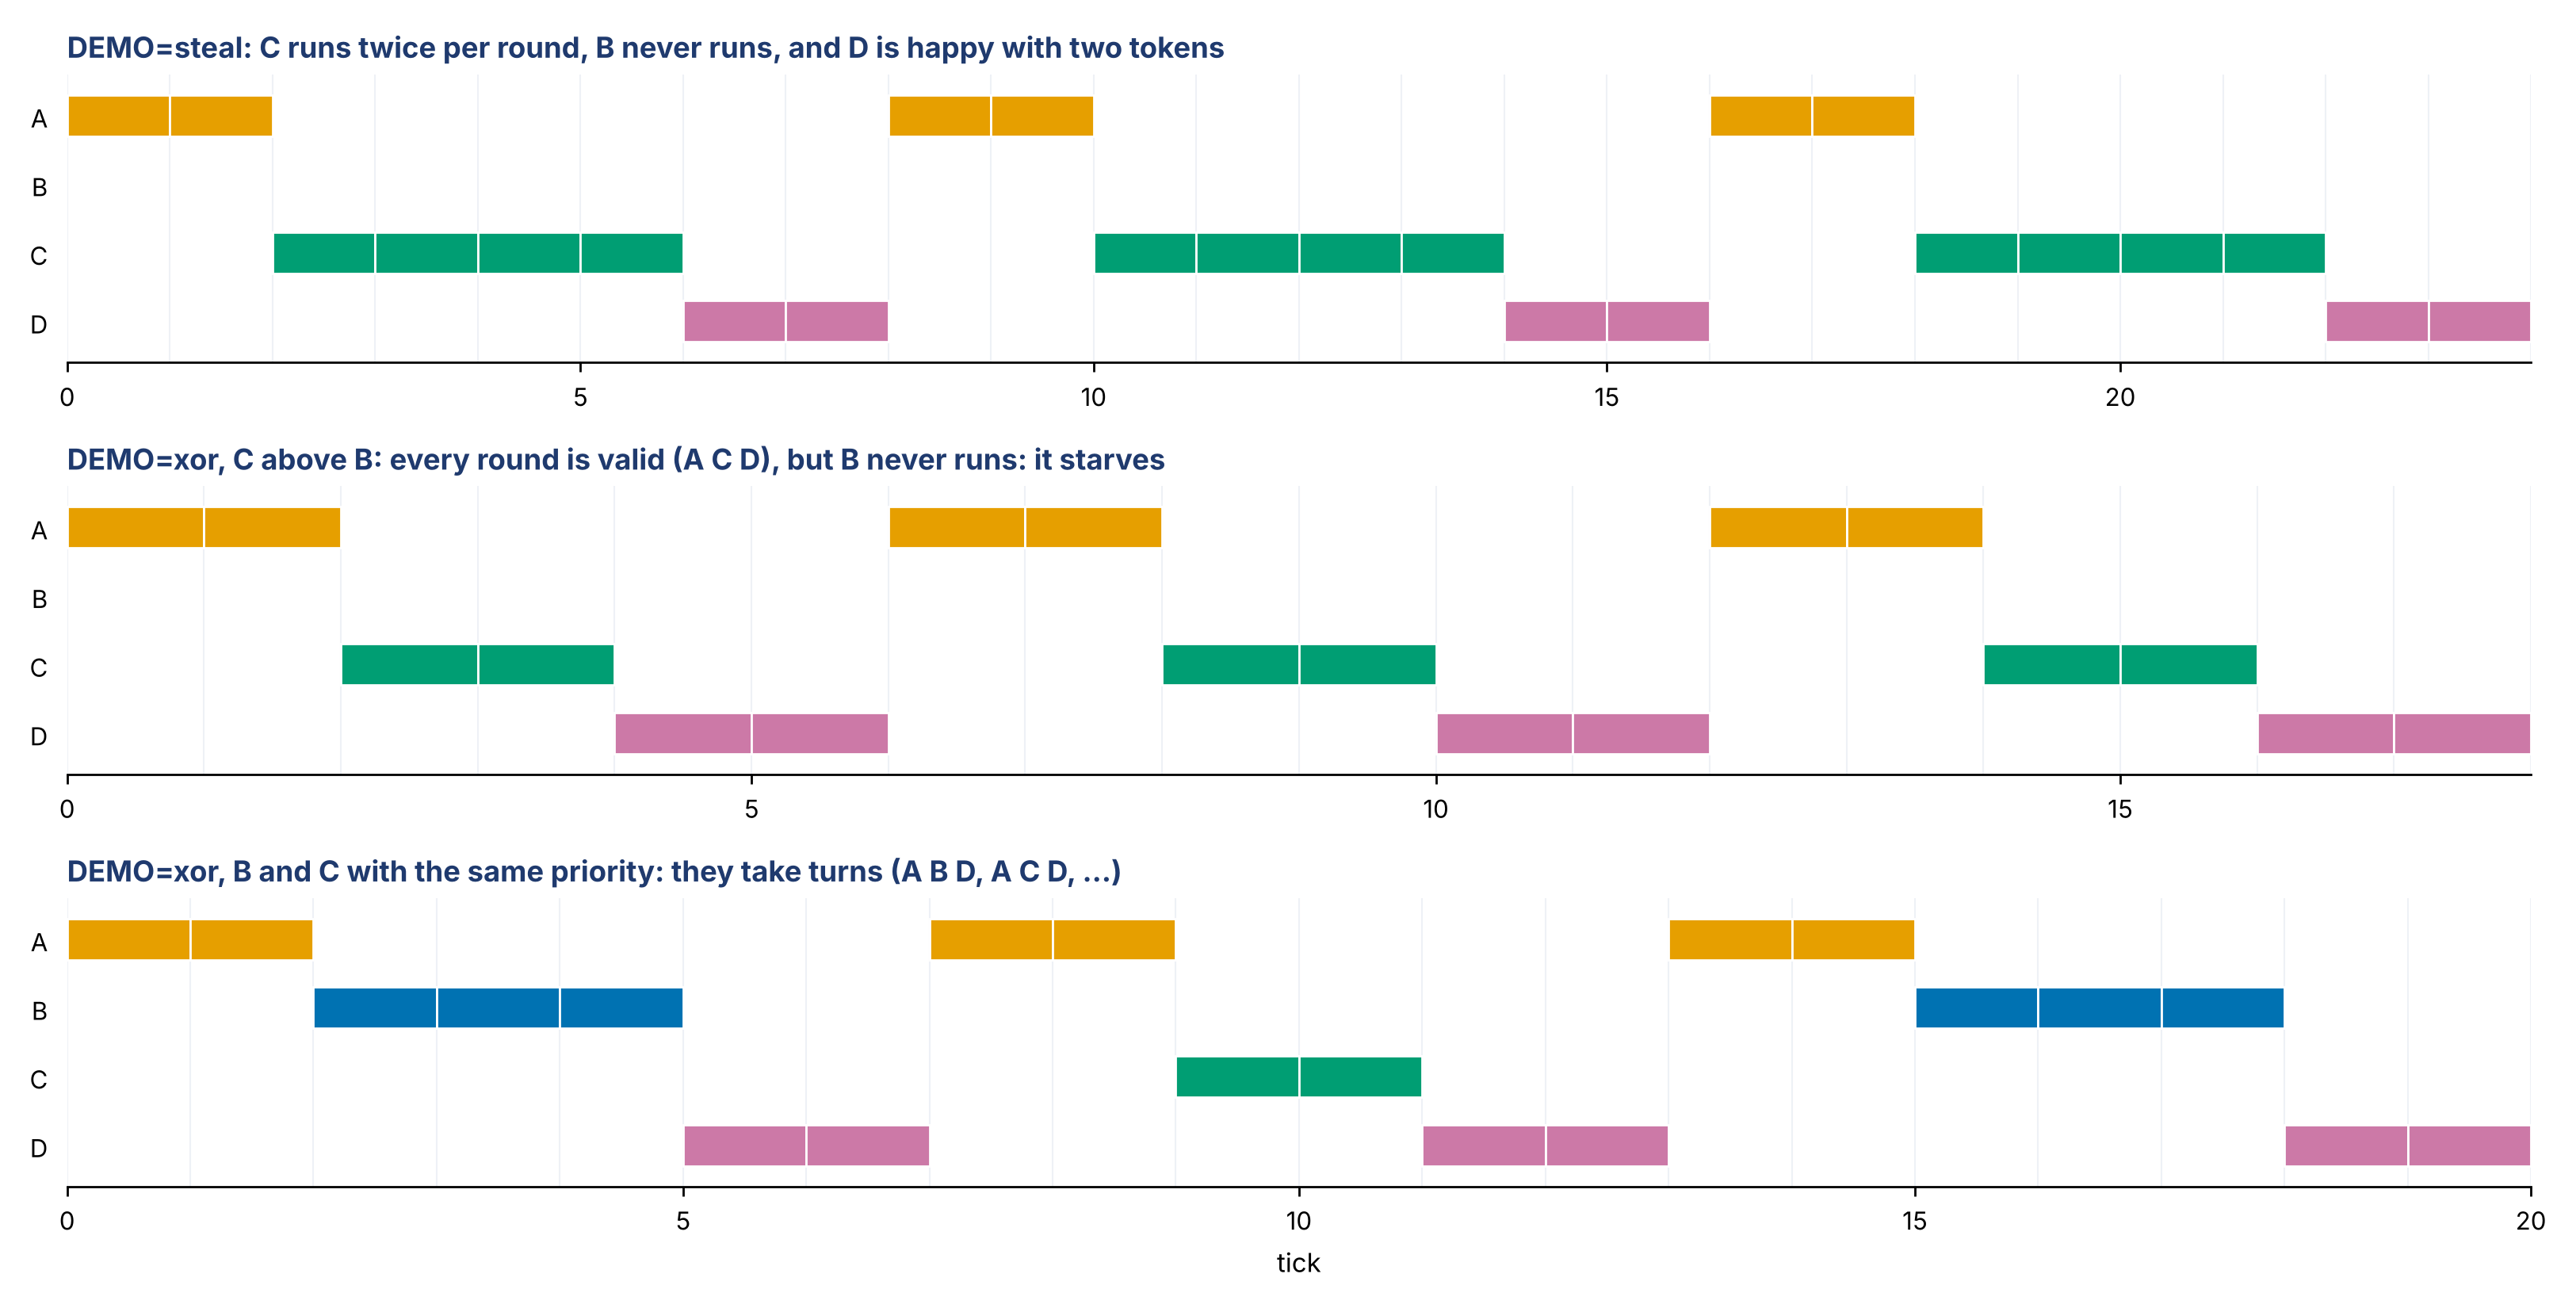
\includegraphics[width=1\textwidth]{contents/images/week-08/steal_xor.png}
    \caption{The \texttt{schedsim} charts of the three runs, redrawn: \texttt{DEMO=steal}, and \texttt{DEMO=xor} with C above B and with B and C at the same priority.}
\end{figure}
\begin{itemize}
    \item Every round is valid: exactly one of B and C, never overlapping.
    \item \textbf{Different priorities: B never runs}. C is always the highest-priority waiter: the graph allows both, the priorities pick, and B \textbf{starves}, as in week 5.
    \item \textbf{Same priority: they take turns}, A B D, A C D, A B D: waiters of equal priority wake in order of arrival, and the one that has just run goes to the back. A design that needs both branches relies on this.
\end{itemize}
\begin{center}
\fbox{\parbox{0.85\textwidth}{\centering The semaphores fix what is \textbf{allowed}; the priorities \textbf{pick} among the allowed orders.}}
\end{center}

\subsection{Inside the kernel: where a blocked task waits}
\begin{figure}[H]
    \centering
    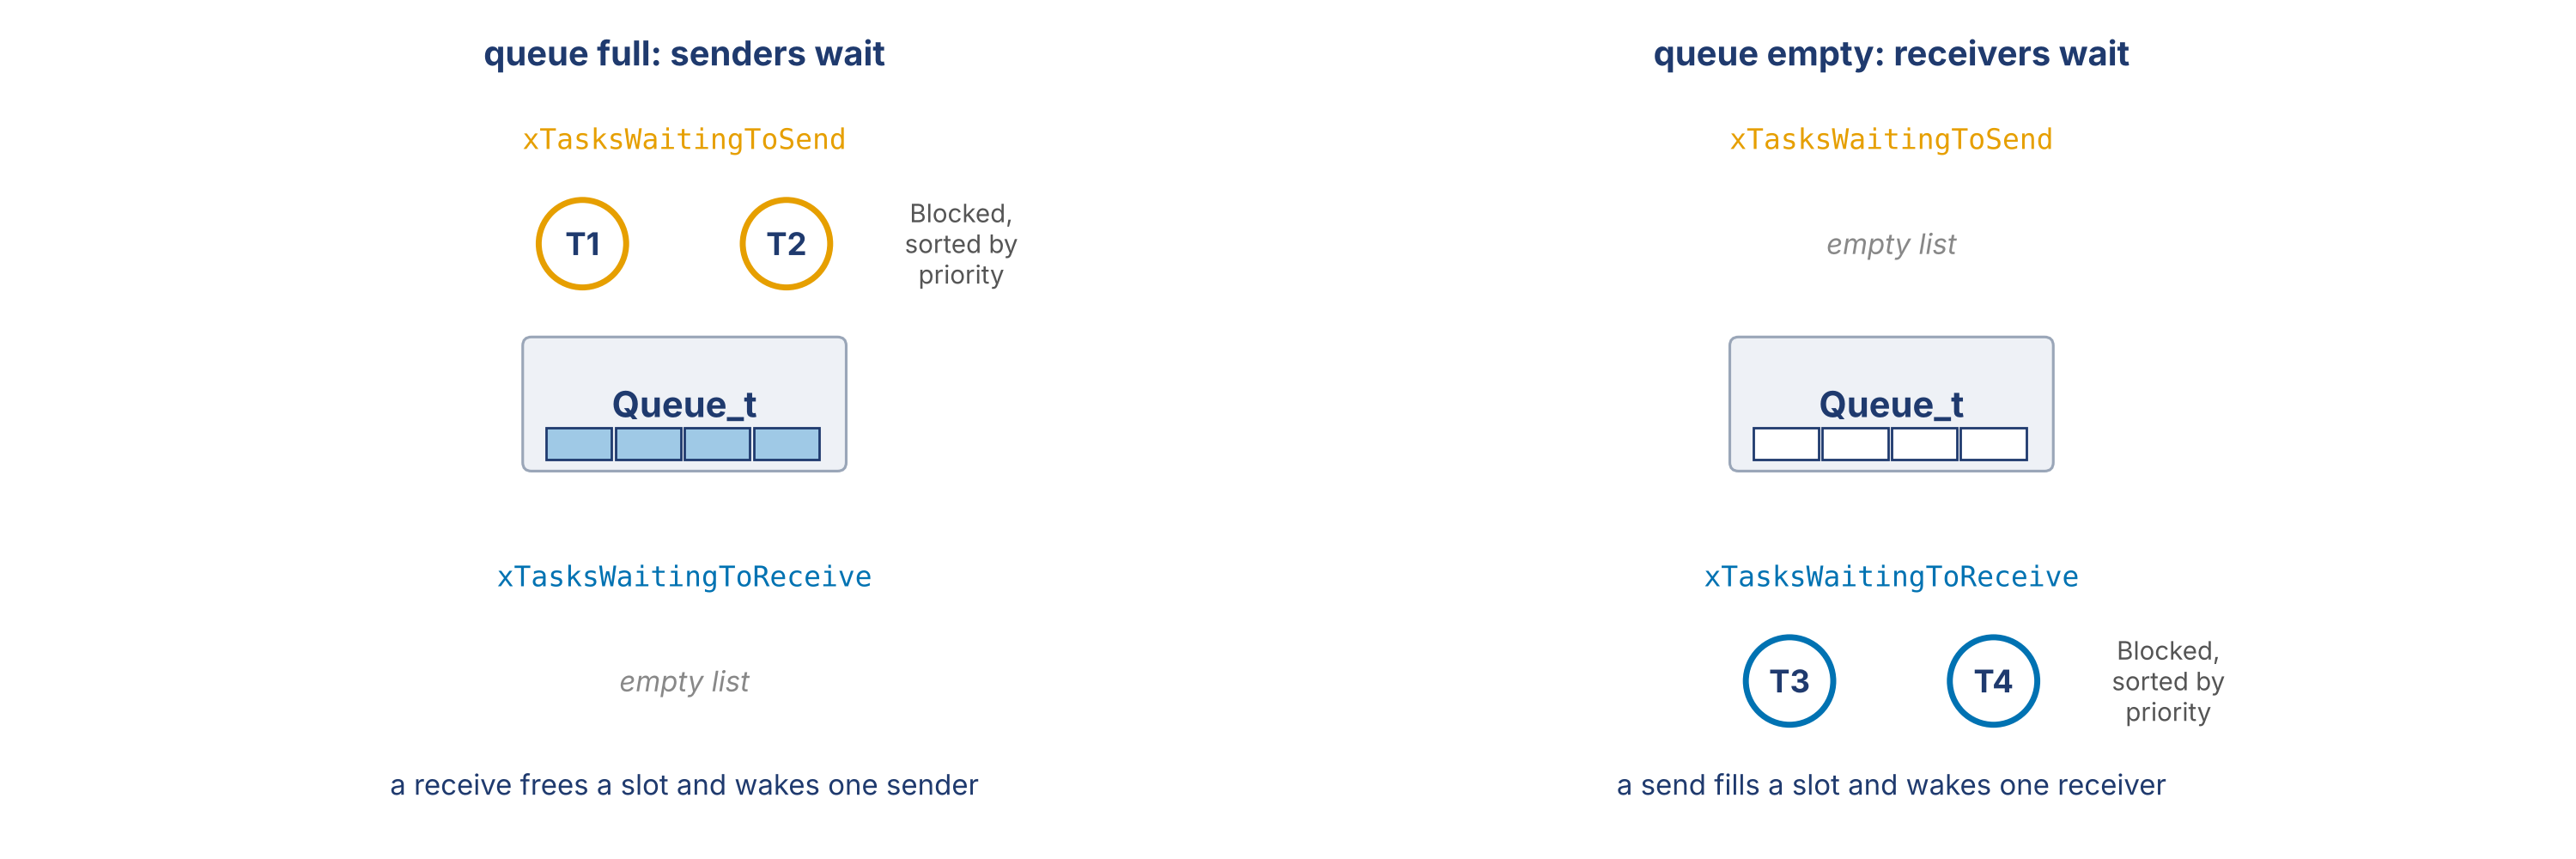
\includegraphics[width=0.85\textwidth]{contents/images/week-08/queue_wait_lists.png}
    \caption{Every queue (\texttt{Queue\_t}) has two wait lists: tasks waiting to send, when it is full, and tasks waiting to receive, when it is empty.}
\end{figure}
\begin{itemize}
    \item A \textbf{semaphore is a queue} with items of size 0, and its count is the number of items: semaphores, mutexes and queues all block and wake in one piece of kernel code.
    \item Each object has its own wait lists, \textbf{sorted by priority}: the head wakes first, and equal priorities keep their order of arrival (the \texttt{xor} runs).
    \item A woken task \textbf{tests again}, because another task may have taken the token first.
\end{itemize}
In class we stop here. The next three sections read the kernel code behind this and behind the trace: they are \textbf{optional}, for study at home.

\subsection{Reading the kernel (optional): the trace module}
How does the trace get its data, with a kernel we never edit? FreeRTOS has \textbf{trace macros}: places in its code where it expands a macro that is empty by default (in \texttt{FreeRTOS.h}), unless your config defines it first. Our \texttt{FreeRTOSConfig.h} does:
\begin{lstlisting}[language=C, showstringspaces=false, basicstyle=\ttfamily\scriptsize]
#define traceTASK_SWITCHED_IN() \
        trace_switched_in( ( uint32_t ) xTickCount, pxCurrentTCB->pcTaskName )
\end{lstlisting}
The kernel expands it in \texttt{vTaskSwitchContext} (\texttt{tasks.c}), right after choosing the next task, and in \texttt{vTaskStartScheduler}, just before the first task starts:
\par\noindent\begin{minipage}[t]{0.4\textwidth}
\begin{lstlisting}[language=C, showstringspaces=false, basicstyle=\ttfamily\scriptsize]
/* tasks.c, vTaskSwitchContext */
taskSELECT_HIGHEST_PRIORITY_TASK();
traceTASK_SWITCHED_IN();
\end{lstlisting}
\end{minipage}\hfill
\begin{minipage}[t]{0.56\textwidth}
\begin{lstlisting}[language=C, showstringspaces=false, basicstyle=\ttfamily\scriptsize]
/* bsp/trace.c, the core of trace_switched_in */
trace_entry_t * e = &entries[ count % TRACE_SIZE ];
e->tick = tick;
e->from = previous;
e->to = name;
count++;
\end{lstlisting}
\end{minipage}
\begin{itemize}
    \item \texttt{entries} is a \textbf{ring buffer} of 256 entries (\texttt{TRACE\_SIZE}), each a tick and two names: when it is full, the newest entry overwrites the oldest.
    \item It stores \textbf{pointers} to the names (they live in the TCBs, which never go away here). \texttt{previous} starts as \texttt{"IDLE"}, hence the first line \texttt{T 0 idle <first task>}. A ``switch'' to the same task is not recorded: the kernel runs \texttt{vTaskSwitchContext} also when the same task goes on.
    \item \texttt{trace\_dump} stops \texttt{recording}, prints \texttt{TRACE BEGIN}, one line per entry and \texttt{TRACE END <tick>} (with \texttt{IDLE} as \texttt{idle}, as the course tool expects), then records again. \texttt{bsp/trace.h} needs only \texttt{<stdint.h>}, because \texttt{FreeRTOSConfig.h} includes it, so it is read inside the kernel's own files.
\end{itemize}
\paragraph{Questions.} (1) \texttt{xTickCount} is \texttt{static} in \texttt{tasks.c}, and \texttt{pcTaskName} needs the layout of \texttt{TCB\_t}, which only \texttt{tasks.c} knows: how can the macro use them? (2) Why does the hook only store three values, instead of printing a line? (3) Where is the printing done, then?
\needspace{4\baselineskip}
\textbf{Solution.}
\begin{enumerate}
    \item \textbf{A macro is text}: the preprocessor pastes it \textbf{inside} \texttt{tasks.c}, where those names are visible. Only \texttt{FreeRTOSConfig.h} changes.
    \item \textbf{The hook runs inside the context switch} (\texttt{vTaskSwitchContext} is called from the PendSV handler \texttt{xPortPendSVHandler}). Printing there would be \textbf{slow} (a formatted line sent byte by byte, which changes the timing you want to measure), \textbf{forbidden} (\texttt{console\_print} enters a critical section, and \texttt{vPortEnterCritical} asserts if called from a handler), and it would \textbf{disturb the switch}, with the kernel between two tasks.
    \item \textbf{Later, in a normal task}: R calls \texttt{trace\_dump} after the last round, with recording stopped so that the record does not change while it is printed.
\end{enumerate}
The general rule inside a context switch: do as little as possible (no printing, no kernel calls, no critical sections), and do the rest later.

\subsection{Reading the kernel (optional): how a task blocks on a semaphore}
\texttt{xSemaphoreTake} (\texttt{include/semphr.h}) is a macro for \texttt{xQueueSemaphoreTake} in \texttt{queue.c}. With some lines left out, and two condensed:
\begin{lstlisting}[language=C, showstringspaces=false, basicstyle=\ttfamily\scriptsize]
for( ; ; )
{
    taskENTER_CRITICAL();
    {
        const UBaseType_t uxSemaphoreCount = pxQueue->uxMessagesWaiting;
        if( uxSemaphoreCount > ( UBaseType_t ) 0 )
        {
            pxQueue->uxMessagesWaiting = uxSemaphoreCount - ( UBaseType_t ) 1;
            ...
            taskEXIT_CRITICAL();
            return pdPASS;
        }
        else if( xTicksToWait == ( TickType_t ) 0 ) { ... return errQUEUE_EMPTY; }
        ...
    }
    taskEXIT_CRITICAL();
    ...
    if( xTaskCheckForTimeOut( &xTimeOut, &xTicksToWait ) == pdFALSE )
    {
        if( prvIsQueueEmpty( pxQueue ) != pdFALSE )
            vTaskPlaceOnEventList( &( pxQueue->xTasksWaitingToReceive ), xTicksToWait );
\end{lstlisting}
In a critical section the task looks at the count: if there is a token, it takes it and returns; if not and the timeout is 0, it fails. Otherwise it checks that the time has not run out, places itself on the wait list of the semaphore, and gives up the CPU.
\begin{itemize}
    \item \emph{What is a semaphore's count, inside the kernel?} \texttt{uxMessagesWaiting}, the number of items: ``Semaphores are queues with a data size of zero'' (a comment in \texttt{queue.c}). A binary semaphore is a queue of length 1 and item size 0, and \texttt{xSemaphoreGive} is a macro for \texttt{xQueueGenericSend}: a send with no data.
    \item \emph{Why the \texttt{for} loop?} \textbf{A woken task tries again}: after the give, or the timeout, it tests the count again, because another task may have taken the token first; if so, it blocks again for the time left, or fails.
    \item \emph{What is different in \texttt{xQueueReceive}?} \textbf{Only the copy}: the same loop, test and \texttt{vTaskPlaceOnEventList}, plus \texttt{prvCopyDataFromQueue}, which copies the item into your variable.
\end{itemize}
So semaphores, mutexes and queues block and wake in \textbf{one single machinery}. The mutex adds the owner, \texttt{u.xSemaphore.xMutexHolder} in \texttt{Queue\_t}; it is a queue of length 1 too, and starts free because \texttt{xQueueCreateMutex} (through \texttt{prvInitialiseMutex}) puts one token in at creation.

\subsection{Reading the kernel (optional): the wait lists, and waking a task}
\texttt{Queue\_t} (\texttt{struct QueueDefinition} in \texttt{queue.c}) contains two lists, each ``Stored in priority order'', and the count:
\begin{lstlisting}[language=C, showstringspaces=false, basicstyle=\ttfamily\scriptsize]
    List_t xTasksWaitingToSend;
    List_t xTasksWaitingToReceive;
    volatile UBaseType_t uxMessagesWaiting;
\end{lstlisting} A task that finds the queue full goes on the first, one that finds it empty on the second; a semaphore uses only the second, since a give never waits. In \texttt{tasks.c}, with some lines left out:
\begin{lstlisting}[language=C, showstringspaces=false, basicstyle=\ttfamily\scriptsize]
void vTaskPlaceOnEventList( List_t * const pxEventList, const TickType_t xTicksToWait )
{
    vListInsert( pxEventList, &( pxCurrentTCB->xEventListItem ) );
    prvAddCurrentTaskToDelayedList( xTicksToWait, pdTRUE );
}

BaseType_t xTaskRemoveFromEventList( const List_t * const pxEventList )
{
    pxUnblockedTCB = listGET_OWNER_OF_HEAD_ENTRY( pxEventList );
    listREMOVE_ITEM( &( pxUnblockedTCB->xEventListItem ) );
    ...
    listREMOVE_ITEM( &( pxUnblockedTCB->xStateListItem ) );
    prvAddTaskToReadyList( pxUnblockedTCB );
    ...
}
\end{lstlisting}
A TCB has two list links: \texttt{xStateListItem} for its \textbf{state} list (ready, delayed, suspended), \texttt{xEventListItem} for the \textbf{wait list of a kernel object}.
\begin{itemize}
    \item \emph{Priorities 1, 3 and 2 wait on an empty queue, and a send arrives: who wakes?} \textbf{Priority 3}: the head of the sorted list. Equal priorities wake in order of arrival, because \texttt{vListInsert} (\texttt{list.c}) places a task after those of the same priority. These are the \texttt{xor} runs: C always won, and with equal priorities B and C took turns.
    \item \emph{Why two lists?} \textbf{One per cause of waking}: the event list for ``it happened'', the delayed list for ``the timeout expired'' (checked at each tick, as for \texttt{vTaskDelay}). Whichever comes first removes the task from both. With \texttt{portMAX\_DELAY} the delayed list is replaced by the suspended list, and no tick wakes it.
    \item \emph{In your week 5 kernel, where would this list live?} \textbf{In the kernel object}: a semaphore would be a struct with its count and its own list of waiters, because the task that signals knows only the semaphore. The \texttt{struct tcb} needs only a link, as \texttt{xEventListItem} in \texttt{TCB\_t}.
\end{itemize}

\subsection{Try it: a fast task and a slow task}
\textbf{Requirement}: a fast producer (1 tick) passes 12 numbers (\texttt{ITEMS}) to a slow consumer (5 ticks) through a buffer of 4 places (\texttt{BUFFER\_SIZE}); both tasks have priority 1. When the buffer is full, the producer must wait without using the CPU. The queue replaces the whole buffer. The consumer is an event-driven task with a delay that makes it slow; the producer makes the numbers, one per tick, then parks itself. It looks at \texttt{uxQueueSpacesAvailable} \textbf{only to print} \texttt{buffer FULL, waits} before the send that blocks: the waiting is done by \texttt{xQueueSend}.
\par\noindent\begin{minipage}[t]{0.42\textwidth}
\begin{lstlisting}[language=C, showstringspaces=false, basicstyle=\ttfamily\scriptsize]
/* outside the functions */
static QueueHandle_t xBuffer;

/* main */
xBuffer = xQueueCreate( BUFFER_SIZE,
                        sizeof( int ) );

/* vConsumer */
for( ;; )
{
    int item;

    xQueueReceive( xBuffer, &item,
                   portMAX_DELAY );
    console_print(
      "consumer: got %2d (tick %lu)\n",
      item,
      ( unsigned long )
        xTaskGetTickCount() );
    vTaskDelay( 5 );
}
\end{lstlisting}
\end{minipage}\hfill
\begin{minipage}[t]{0.55\textwidth}
\begin{lstlisting}[language=C, showstringspaces=false, basicstyle=\ttfamily\scriptsize]
/* vProducer: makes the 12 numbers, and says so
 * when it finds the buffer full */
for( int i = 1; i <= ITEMS; i++ )
{
    if( uxQueueSpacesAvailable( xBuffer ) == 0 )
    {
      console_print(
        "producer: %2d, buffer FULL, waits"
        " (tick %lu)\n", i,
        ( unsigned long ) xTaskGetTickCount() );
    }

    xQueueSend( xBuffer, &i, portMAX_DELAY );
    console_print( "producer: put %2d (tick %lu)\n",
      i, ( unsigned long ) xTaskGetTickCount() );
    vTaskDelay( 1 );
}
\end{lstlisting}
\end{minipage}
\begin{figure}[H]
    \centering
    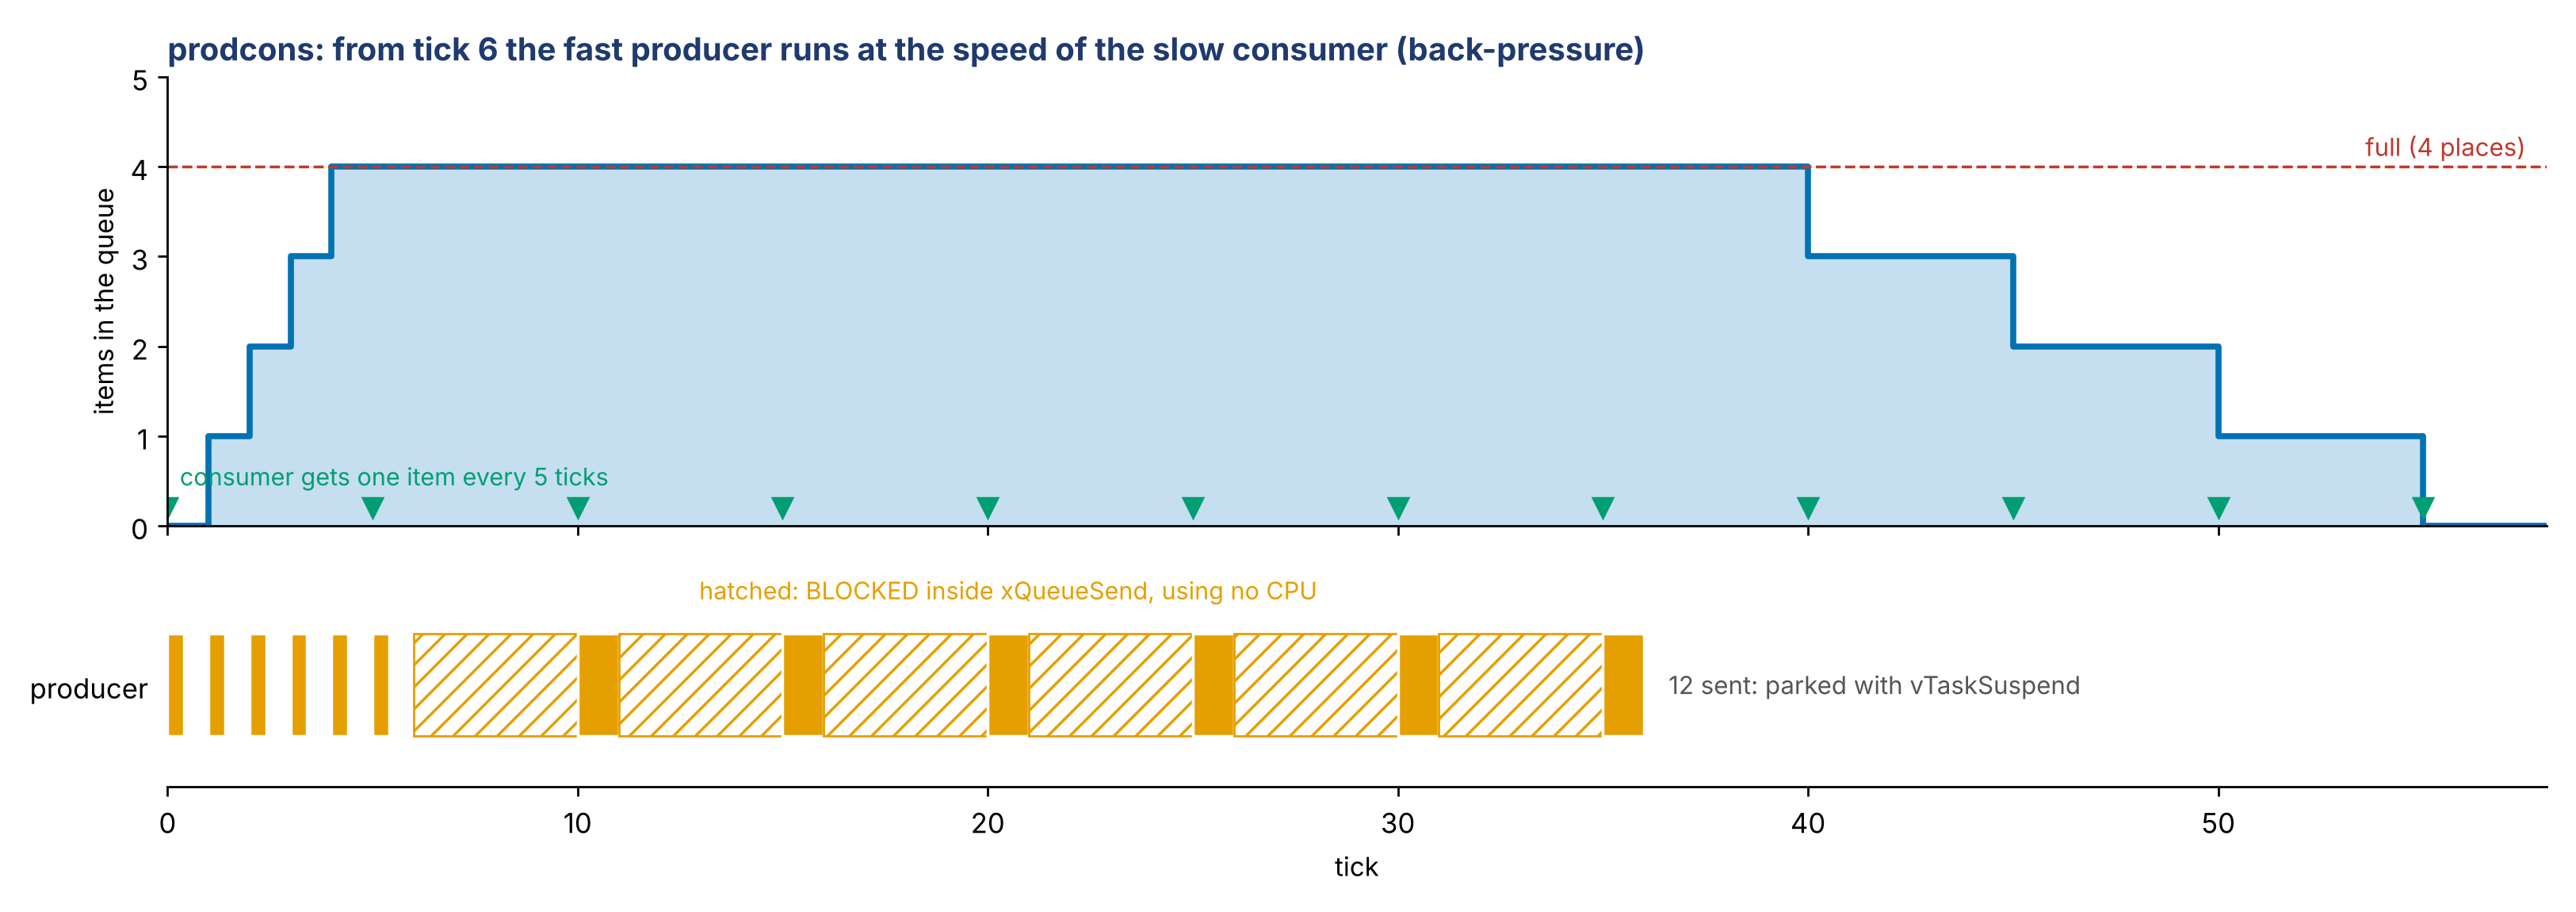
\includegraphics[width=1\textwidth]{contents/images/week-08/prodcons_fill.png}
    \caption{The run of \texttt{make APP=prodcons run}, reconstructed from its output (\texttt{put 1} \dots\ \texttt{got 12} at tick 55): the items in the queue, the consumer's receives every 5 ticks, and the producer, BLOCKED in \texttt{xQueueSend} from tick 6 until the 12th number is sent.}
\end{figure}
\begin{itemize}
    \item Ticks 1 to 4: the producer is faster, and 2, 3, 4, 5 fill the four places; at tick 5 the consumer frees one just in time, so 6 goes in without waiting. From tick 6 (\texttt{producer: 7, buffer FULL, waits}) the producer blocks inside \texttt{xQueueSend}, using no CPU.
    \item Then every 5 ticks a receive frees one place and wakes the producer: the fast task runs at the speed of the slow one. This is \textbf{back-pressure}: a full buffer slows down the task that fills it.
    \item After 12: the producer is parked with \texttt{vTaskSuspend}, the consumer blocks in \texttt{xQueueReceive}, the idle task runs. No loop tests the buffer and no lock appears in the code: the queue does it all.
\end{itemize}

\subsection{Try it: the same buffer, by hand}
\textbf{Requirement}: with \texttt{DEMO=sem}, the same behaviour without a queue: the \texttt{empty}, \texttt{full}, \texttt{mutex} solution of Unit 1, with an array \texttt{buffer} and two indexes \texttt{in} and \texttt{out}.
\begin{lstlisting}[language=C, showstringspaces=false, basicstyle=\ttfamily\scriptsize]
/* main, DEMO_SEM */
empty = xSemaphoreCreateCounting( BUFFER_SIZE, BUFFER_SIZE );
full  = xSemaphoreCreateCounting( BUFFER_SIZE, 0 );
mutex = xSemaphoreCreateMutex();

/* vProducer, DEMO_SEM: the send becomes the code of Unit 1 */
xSemaphoreTake( empty, portMAX_DELAY );
xSemaphoreTake( mutex, portMAX_DELAY );
buffer[ in ] = i;
in = ( in + 1 ) % BUFFER_SIZE;
xSemaphoreGive( mutex );
xSemaphoreGive( full );
\end{lstlisting}
The full-buffer test uses \texttt{uxSemaphoreGetCount(~empty~)} in place of \texttt{uxQueue\-Spaces\-Available}, and the consumer is the mirror image (take \texttt{full}, take \texttt{mutex}, read \texttt{buffer[ out ]}, give \texttt{mutex}, give \texttt{empty}). Run \texttt{make APP=prodcons DEMO=sem run}: \textbf{exactly the same lines as with the queue}, tick by tick; only the banner differs. So the queue does all this for you:
\begin{center}
\small
\begin{tabular}{P{0.3} P{0.55}}
    \hline
    \textbf{your semaphores} & \textbf{inside the queue} \\
    \hline
    \texttt{full} (count and waiters) & the number of items, and the list of tasks waiting to receive \\
    \texttt{empty} (count and waiters) & the number of free places, and the list of tasks waiting to send \\
    \texttt{mutex} & a short critical section in the kernel, around the copy \\
    \texttt{buffer}, \texttt{in}, \texttt{out} & the queue's own memory, with its read and write positions \\
    \hline
\end{tabular}
\end{center}

\subsection{The gatekeeper}
An execution model you need to understand. Last week the output mixed because several tasks wrote to the same UART: a write is not atomic, and depends on how \texttt{printf} processes its buffer. We surrounded it with a spinlock; in FreeRTOS a mutex would do. \textbf{Lock it, or give the resource one owner}: the gatekeeper makes the resource \textbf{not shared}, which is much better.
\begin{itemize}
    \item A \textbf{gatekeeper} is the \textbf{only} task allowed to touch a resource; the others ask it, by sending messages to a queue. As in real life: to share something, set an access rule, or name a \textbf{manager}.
    \item S1 and S2 build a whole line in a \textbf{local variable} and send a copy to the queue; they never touch the UART. The task \texttt{gate} takes the lines one by one and writes each with \texttt{uart\_write}: only one task uses the UART, so \textbf{no lock} and nothing can mix.
    \item Any mechanism could carry the data; in FreeRTOS the natural one is a \textbf{queue}. The gatekeeper is a very ``stupid'' task: a loop that reads the queue and, when there is something, prints it.
\end{itemize}
\begin{figure}[H]
    \centering
    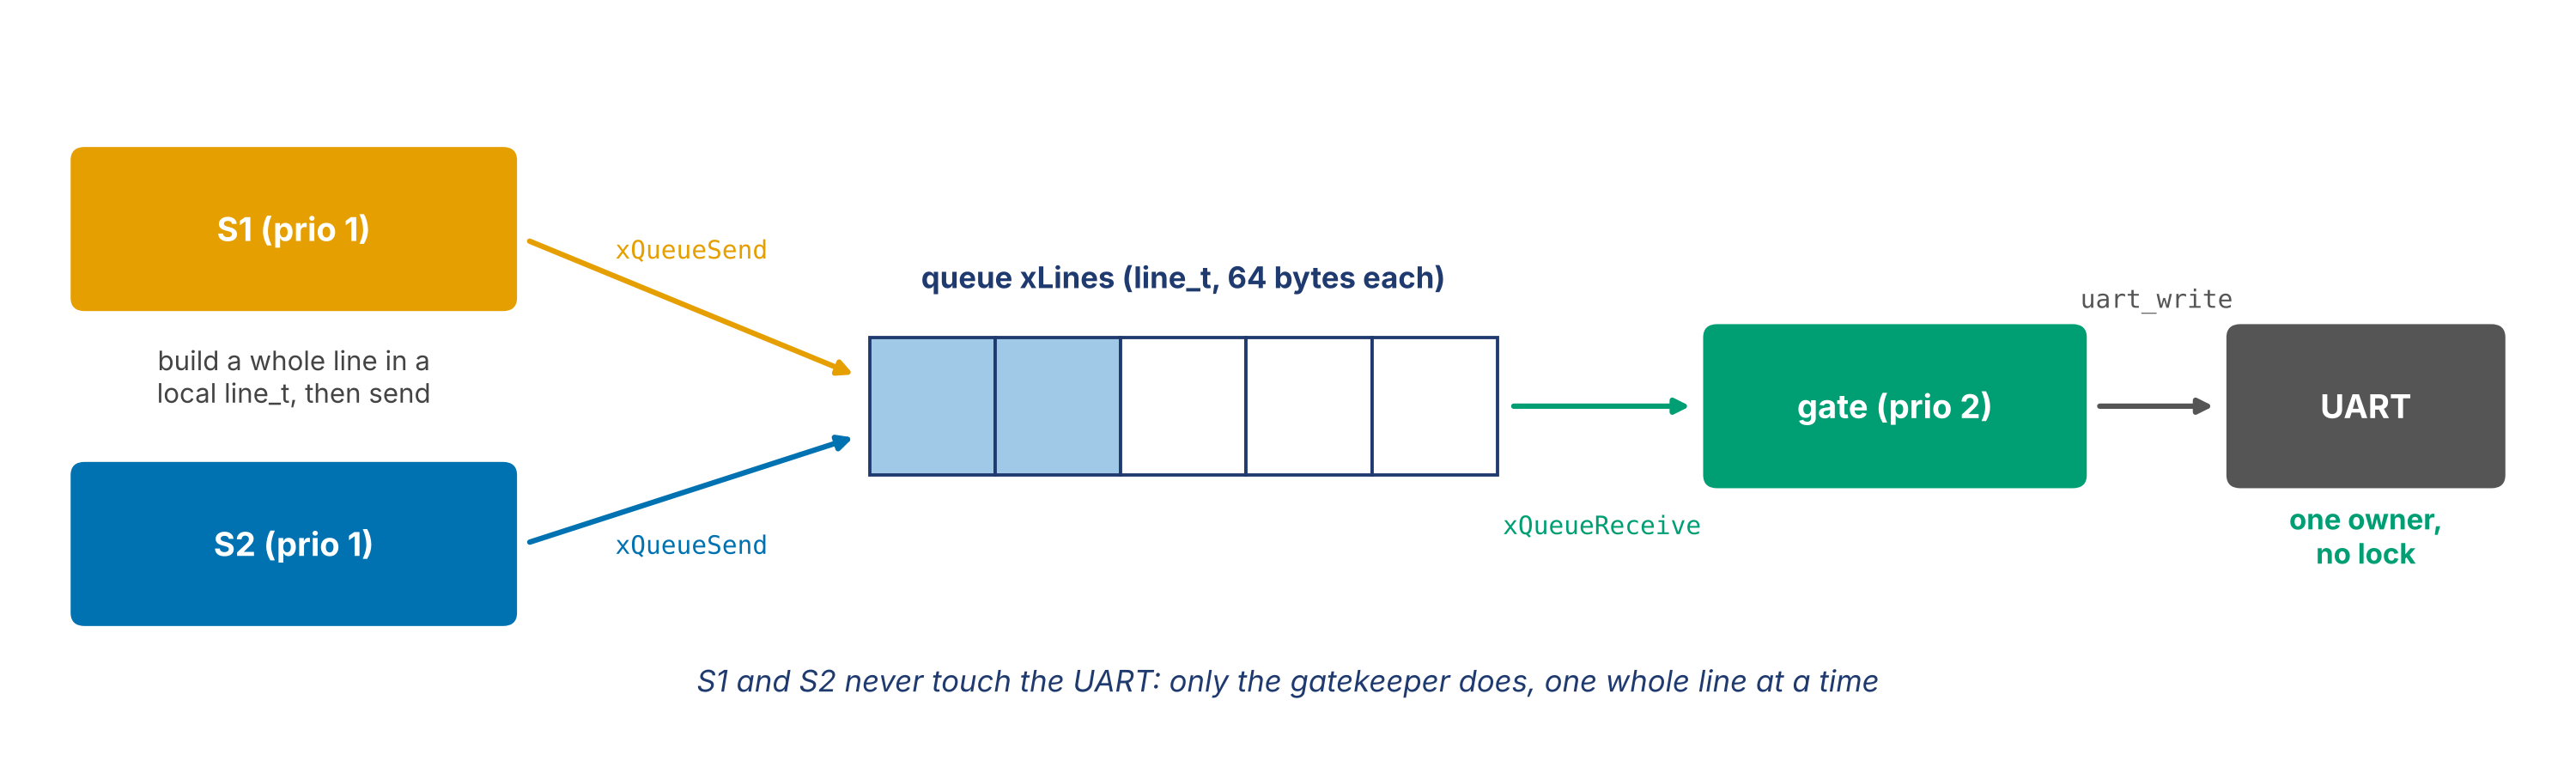
\includegraphics[width=0.95\textwidth]{contents/images/week-08/gatekeeper.png}
    \caption{The gatekeeper: one owner instead of sharing. The senders send messages; only \texttt{gate} writes to the UART.}
\end{figure}
Given in \texttt{apps/gatekeeper.c}: the message \texttt{line\_t}, of fixed size (64 bytes, \texttt{LINE\_SIZE}) so that the queue can copy it; \texttt{QUEUE\_LENGTH}, 8 lines; \texttt{sender\_t} with \texttt{sender1} (a line every 7 ticks) and \texttt{sender2} (every 11). Both senders run \texttt{vSender}, told apart by the parameter. The gatekeeper has priority 2, the senders 1: it sleeps on an empty queue, and runs at once when a line arrives.

\paragraph{Try it: one task owns the UART.} \textbf{Requirement}: whole lines reach the UART and never mix, with no lock on it.
\par\noindent\begin{minipage}[t]{0.44\textwidth}
\begin{lstlisting}[language=C, showstringspaces=false, basicstyle=\ttfamily\scriptsize]
/* outside the functions */
static QueueHandle_t xLines;

/* main */
xLines = xQueueCreate( QUEUE_LENGTH,
                       sizeof( line_t ) );

/* vGatekeeper */
for( ;; )
{
    line_t msg;

    xQueueReceive( xLines, &msg,
                   portMAX_DELAY );
    uart_write( msg.text,
                strlen( msg.text ) );
}
\end{lstlisting}
\end{minipage}\hfill
\begin{minipage}[t]{0.53\textwidth}
\begin{lstlisting}[language=C, showstringspaces=false, basicstyle=\ttfamily\scriptsize]
/* vSender: S1 and S2 run the same code */
unsigned n = 0;
for( ;; )
{
    line_t msg;

    snprintf( msg.text, sizeof msg.text,
        "%s: line %u, tick %lu, "
        "aaaaaaaaaa bbbbbbbbbb cccccccccc\n",
        me->name, n,
        ( unsigned long ) xTaskGetTickCount() );
    n++;

    xQueueSend( xLines, &msg, portMAX_DELAY );
    vTaskDelay( me->period );
}
\end{lstlisting}
\end{minipage}

\noindent Sending a local variable is fine here: the queue copies the 64 bytes, not a pointer, and \texttt{snprintf} never writes more than the message size. The sender stack is \textbf{twice} the usual size, because \texttt{snprintf} and the message live on it.

\paragraph{From class: the queue length.} The creation is the \textbf{most sensitive line}. \emph{Why?} (A question to the class.) With a length of \textbf{1}, printing becomes a mutual exclusion: once one task has printed, the next must wait until the gatekeeper runs and empties the queue. A longer queue is a \textbf{buffer}: printing is just a copy into memory, very fast, and the task goes on, while the UART is very slow (a task with a 10\,ms budget cannot spend 10\,ms on a character). You rely on the gatekeeper getting \textbf{enough CPU}; in the professor's view it usually has a low priority, and still manages. Whenever one task is slow and the others must go fast, the gatekeeper is a good model.

\paragraph{Tracing works the same way.} FreeRTOS's tracing \textbf{logs events in memory} (a queue is a perfect example), and a very-low-priority task, often the idle task, prints them or saves them to flash. In embedded systems practically every slow job is handled this way.

\paragraph{Run it.} Let \texttt{make APP=gatekeeper run} go for a few seconds:
{\verbatimscriptsize
\begin{verbatim}
gatekeeper: S1 and S2 send lines, only the gatekeeper prints
S1: line 0, tick 0, aaaaaaaaaa bbbbbbbbbb cccccccccc
S2: line 0, tick 0, aaaaaaaaaa bbbbbbbbbb cccccccccc
S1: line 1, tick 7, aaaaaaaaaa bbbbbbbbbb cccccccccc
S2: line 1, tick 11, aaaaaaaaaa bbbbbbbbbb cccccccccc
...
\end{verbatim}}
\begin{itemize}
    \item \textbf{No line is mixed}: in a 32\,s run, all 748 lines were whole. S1 and S2 never call \texttt{console\_print} or \texttt{uart\_write}, so its critical section (week 7) is not used once the tasks run; the banner is printed by \texttt{main} before the scheduler starts.
    \item With a \textbf{lower} priority than the senders, the lines are still whole, but the gatekeeper runs only when both senders sleep; if they sent faster than it writes, the queue would fill and the senders would block: back-pressure, not a mix.
\end{itemize}

\paragraph{Three fixes for mixed output.}
\begin{center}
\footnotesize
\begin{tabular}{P{0.13} P{0.24} P{0.24} P{0.26}}
    \hline
    & \textbf{spinlock (week 7, Unit 2)} & \textbf{critical section (week 7, Unit 3)} & \textbf{gatekeeper} \\
    \hline
    who waits & the other task, spinning on the CPU (or yielding and retrying) & nobody can even ask: no switch can happen until the section ends & a sender, BLOCKED, only if the queue is full \\
    interrupts masked? & no & yes, with BASEPRI, while the line goes out: the tick waits too & no, except for the kernel's short copy into and out of the queue \\
    cost & CPU wasted while spinning & no task and no tick for the whole line & one more task, a queue, copies of messages \\
    good for & short sections, no blocking kernel & very short sections & slow resources, such as a UART \\
    \hline
\end{tabular}
\end{center}
Slow work in a critical section delays the whole system; a gatekeeper delays only its senders, and only when its queue is full.

\paragraph{Homework, and a warning.} These programs have \textbf{zero complexity} as C code (a few lines are no problem in a master's degree); the complexity is in the organisation: where the semaphores are created, who signals, who waits. Do all the exercises of the week and the lab. If you find the C code too complex, \textbf{tell the professor now}: ``if you do not tell me there is a problem, I cannot solve it''.

\section{Unit 2: summary}
\begin{itemize}
    \item \textbf{Four blocking primitives}: binary semaphore (0 or 1, starts empty: to signal), counting semaphore (0 to max, any start), mutex (one token with an owner, starts free: to protect data), queue (N items, copied in and out). Semaphores share \texttt{SemaphoreHandle\_t}, \texttt{xSemaphoreTake}, \texttt{xSemaphoreGive}; the queue has \texttt{QueueHandle\_t}, \texttt{xQueueSend}, \texttt{xQueueReceive}. Pick the object from the requirement.
    \item \textbf{The event-driven task}: a loop that blocks on a take or a receive, using no CPU, and runs when its event arrives (the aperiodic model).
    \item \textbf{Timeouts and return codes}: 0 does not wait, \texttt{pdMS\_TO\_TICKS( ms )} waits at most that long, \texttt{portMAX\_DELAY} for ever. With a finite timeout always test the return code; after a failure you hold nothing.
    \item \textbf{In code}: semaphores are \texttt{static} globals, created once (here in \texttt{main}); a task function never returns. The semaphores decide what is allowed, the priorities pick: a shared token is stolen by the highest-priority waiter, and an exclusive fork can starve a branch.
    \item \textbf{Inside the kernel}: a semaphore is a queue of items of size 0; every object has wait lists sorted by priority, and a woken task tests again. Optionally: \texttt{traceTASK\_SWITCHED\_IN} is a macro pasted inside \texttt{tasks.c}, \texttt{trace\_switched\_in} only stores three values, and \texttt{trace\_dump} prints them later, from a task.
    \item \textbf{The queue} is the bounded buffer in one object, with back-pressure; \texttt{DEMO=sem} gives exactly the same run by hand.
    \item \textbf{The gatekeeper}: one task owns the UART, the others send it whole lines through a queue; no lock, no mixed output. Size the queue so that senders rarely block; the same idea serves tracing and logging.
\end{itemize}

\section{Unit 3 - Deadlock and message passing}
The second lecture closes the first part on synchronization with a problem that is theoretical, but needs real solutions when it happens in an application: \textbf{deadlock}. Paths as in Unit 2.

\subsection{Tasks that wait for each other}
A deadlock needs at least two tasks that each need more than one resource. The typical case: two tasks take two semaphores in \textbf{opposite orders}. Some runs stop for ever, with no error:
\begin{lstlisting}[basicstyle=\ttfamily\footnotesize]
semaphore S = 1, Q = 1;
T1:  wait( S );  print A;  wait( Q );  ...
T2:  wait( Q );  print C;  wait( S );  ...
\end{lstlisting}
If both pass their first wait, T1 holds \texttt{S} and waits for \texttt{Q}, T2 holds \texttt{Q} and waits for \texttt{S}: the signals are further on, and neither ever gets there. Only some interleavings do this: bad luck.
\begin{itemize}
    \item A \textbf{deadlock} is a set of tasks in which each one waits for something that only another task of the set can provide. Nobody in the set can ever run again. No fault and no error appear: the tasks are simply BLOCKED, and the rest of the system keeps running.
    \item \textbf{Starvation} may look similar, but a starving task \textbf{could} run: others always go first (week 5). It is a performance problem of the \textbf{OS} (its scheduler); deadlock is fixed in the \textbf{synchronization scheme of the application}.
\end{itemize}

\subsection{The four necessary conditions}
A deadlock can happen only if \textbf{all four} hold at the same time (Coffman, 1971):
\begin{enumerate}
    \item \textbf{Mutual exclusion}: a resource can be used by only one task at a time.
    \item \textbf{Hold and wait}: a task holds at least one resource while it waits for another.
    \item \textbf{No preemption}: a resource cannot be taken away from its holder; the holder must give it back.
    \item \textbf{Circular wait}: a cycle of tasks T1, \dots, Tn, each waiting for a resource held by the next, and Tn for one held by T1.
\end{enumerate}
T1 and T2 above have all four: a semaphore at 1 lets one task in; T1 holds \texttt{S} and waits for \texttt{Q}; only the holder signals; T1 waits for T2 and T2 for T1. \textbf{Necessary} means: remove any one, and no deadlock is possible. That is \textbf{prevention}: when writing an application, if all four are there a deadlock is possible, so make sure one is missing.
\begin{itemize}
    \item \emph{Which FreeRTOS feature of yesterday does the third condition recall?} The \textbf{timeout}: ``if you set a timer, there is preemption'', and if every wait has a timeout, no task waits for ever\footnote{More precisely: the timeout does not take a resource away from its holder; it makes the \textbf{waiting} task give up. The cycle breaks only if that task also \textbf{gives back} what it holds, as the slides put it under ``no preemption''. Even then the tasks can keep failing together (livelock): see \texttt{DEMO=timeout} below.}.
\end{itemize}

\subsection{Resource-allocation graph}
A \textbf{resource-allocation graph} (RAG) shows who holds what and who waits for what (the symbols are the professor's choice, not a standard): \textbf{circles} are tasks, \textbf{squares} resources; a \textbf{request} edge, task $\rightarrow$ resource (dashed), says the task waits for it; an \textbf{assignment} edge, resource $\rightarrow$ task (solid), says the task holds it.
\begin{figure}[H]
    \centering
    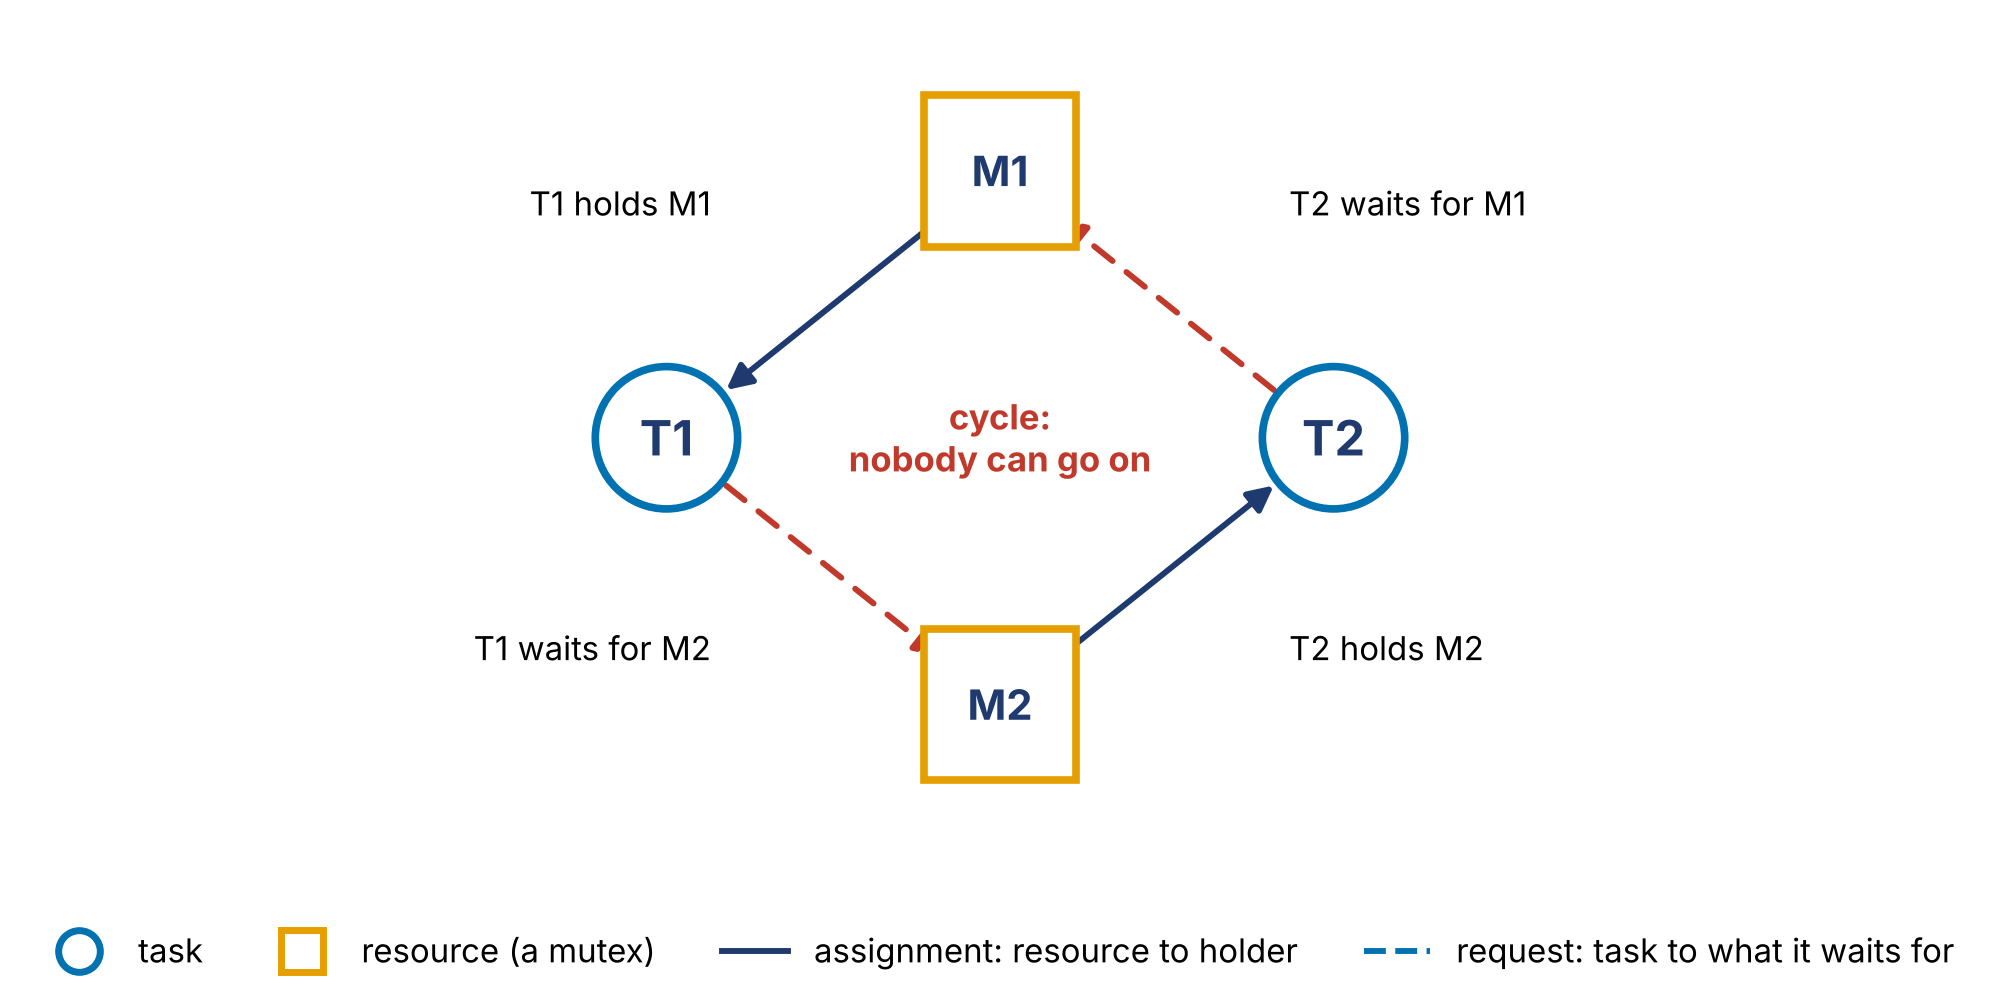
\includegraphics[width=0.65\textwidth]{contents/images/week-08/rag_basic.png}
    \caption{T1 holds M1 and needs M2; T2 holds M2 and needs M1. The cycle means nobody can go on.}
\end{figure}
With \textbf{one unit} per resource, as a mutex: a cycle means deadlock, and no cycle means no deadlock.

\paragraph{Try it on paper: read the graph.} Each resource has one unit unless stated; a dot marks each unit of a resource with two. Is there a deadlock in each graph?
\begin{figure}[H]
    \centering
    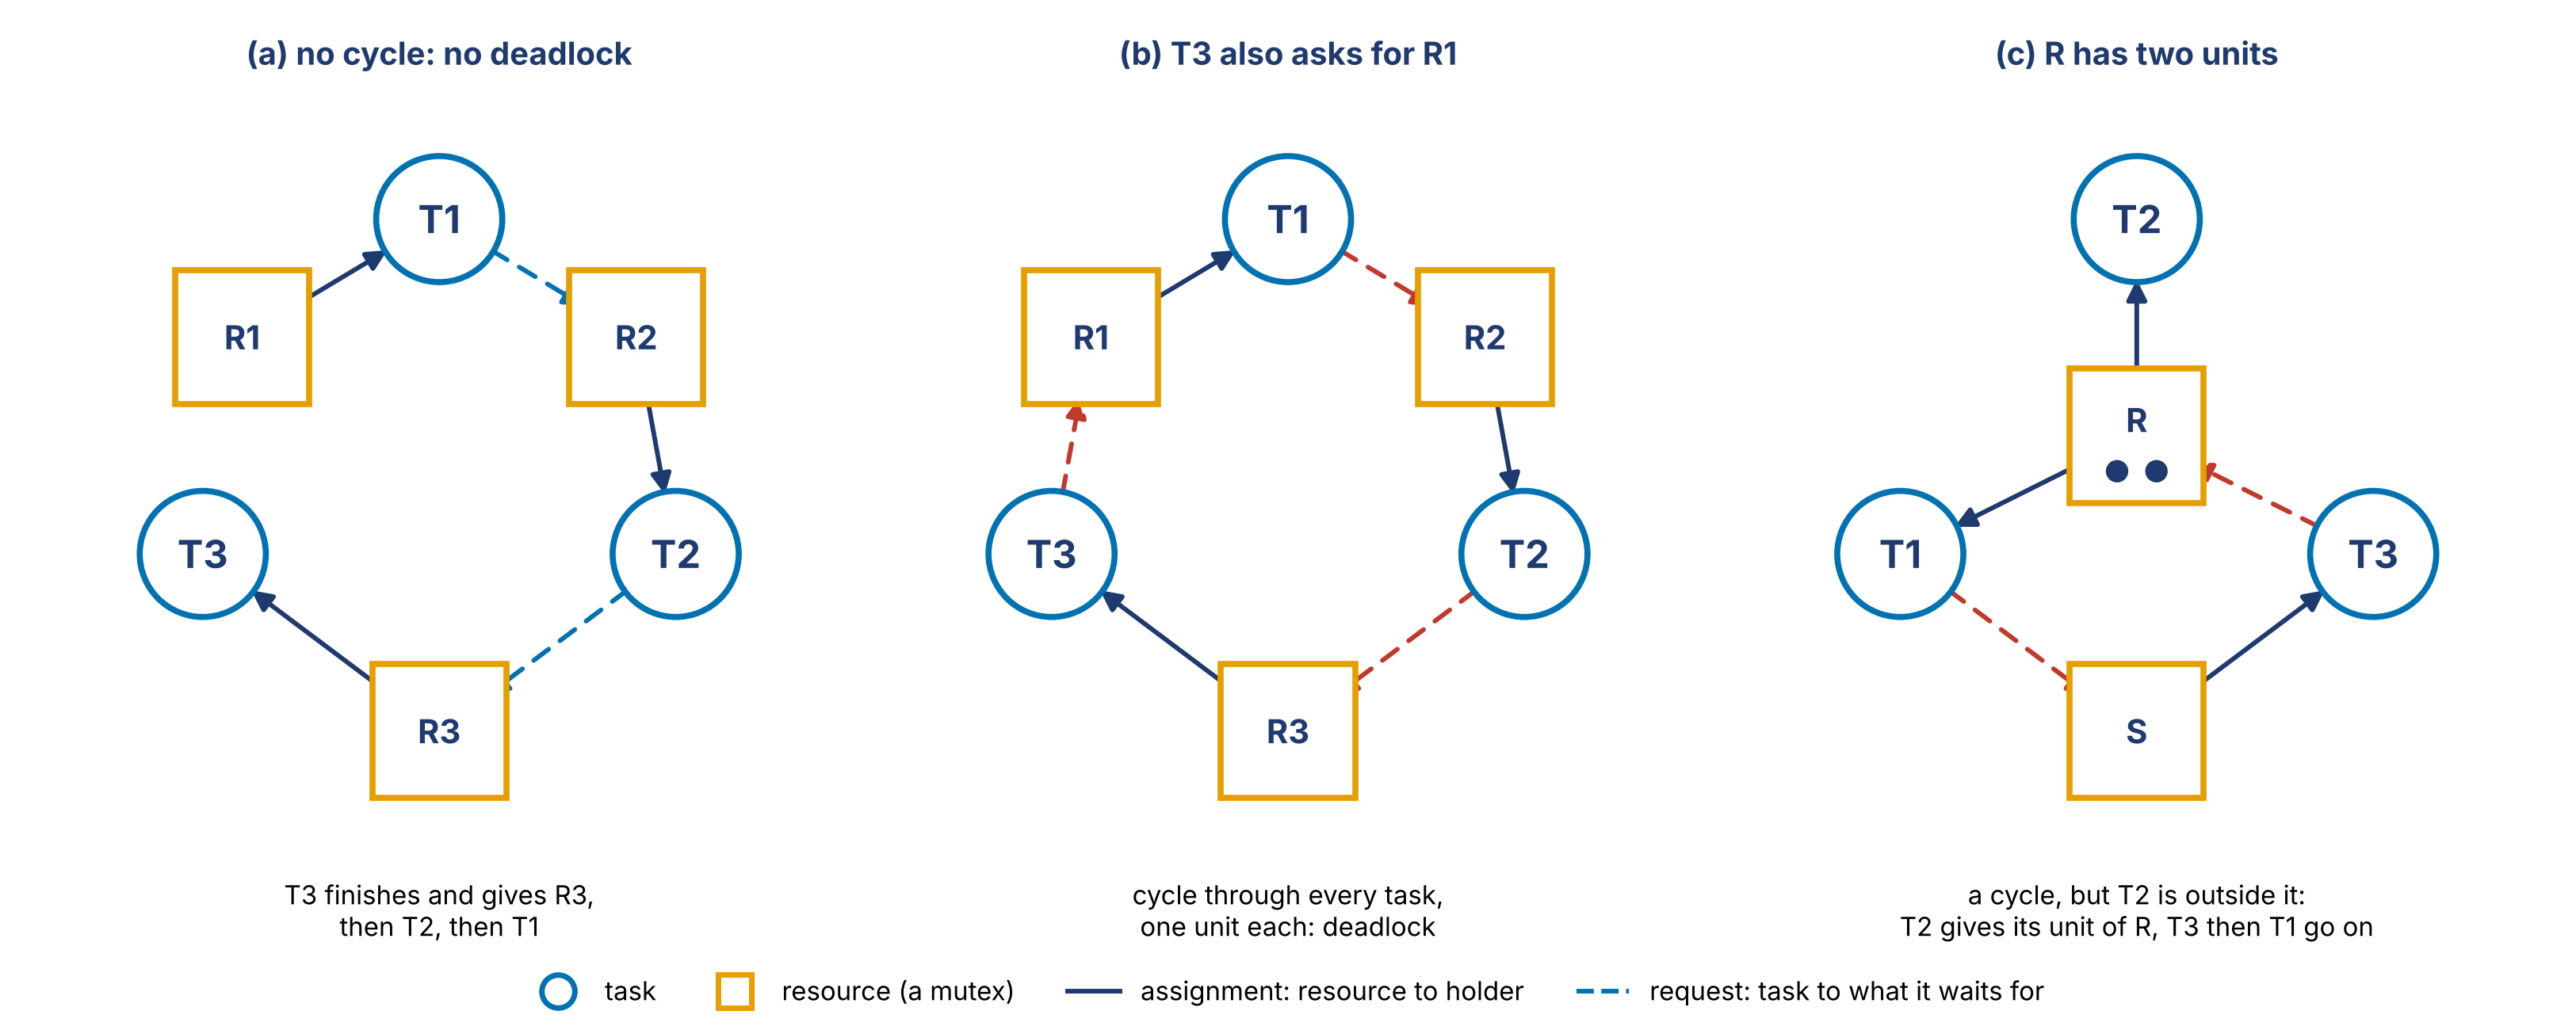
\includegraphics[width=1\textwidth]{contents/images/week-08/rag_examples.png}
    \caption{The three graphs of the slide, with the answers. Red dashed edges are the requests that close a cycle.}
\end{figure}
\begin{itemize}
    \item \textbf{(a) No deadlock}: no cycle. T3 needs nothing else, finishes and frees R3; then T2 frees R2; then T1 completes.
    \item \textbf{(b) Deadlock}: T3 also asks for R1, held by T1. The cycle goes through every task, and every resource has one unit.
    \item \textbf{(c) No deadlock, although there is a cycle}: R has two units, held by T1 and T2. T3 waits for R, T1 waits for S held by T3; but T2 is outside the cycle, finishes and frees one unit of R; T3 gets it, finishes and frees S; T1 runs.
\end{itemize}
With several units a cycle is \textbf{necessary but not sufficient}: with single units you just look for a loop, with several you must reason on what each task can do.

\subsection{Three ways to handle deadlock}
\begin{center}
\small
\begin{tabular}{P{0.22} P{0.27} P{0.38}}
    \hline
    \textbf{strategy} & \textbf{when it acts} & \textbf{the idea} \\
    \hline
    prevention & when you write the code & make one of the four conditions impossible \\
    avoidance & at each request, at run time & grant a request only if the system stays safe \\
    detection and recovery & after it has happened & notice the deadlock, then break it \\
    \hline
\end{tabular}
\end{center}
The run-time cost \textbf{grows} down the table: avoidance and detection run code that steals CPU cycles. Embedded systems mostly use \textbf{prevention}: no run-time cost, simple to check by reading the code, and a product cannot wait for someone to reboot it. With few resources, put the pressure on the \textbf{developer}, not on the platform.

\needspace{8\baselineskip}
\paragraph{Prevention: break one condition.}
\begin{center}
\small
\begin{tabular}{P{0.15} P{0.42} P{0.33}}
    \hline
    \textbf{condition} & \textbf{how to break it} & \textbf{the limit} \\
    \hline
    mutual exclusion & make the resource shareable, or give it one owner (a gatekeeper, so no lock at all) & not every resource allows it \\
    hold and wait & take all the resources at once, or hold nothing when you wait for another & you must know them all in advance; resources stay idle for longer \\
    no preemption & if the second take fails, give back what you hold, and retry later & the work done so far may have to be redone \\
    circular wait & lock ordering: all tasks take resources in one global order & every programmer must follow the rule \\
    \hline
\end{tabular}
\end{center}
From class:
\begin{itemize}
    \item \textbf{Mutual exclusion}: yesterday's \textbf{gatekeeper} turns the mutual exclusion on the UART into a \textbf{communication}: no semaphore around the resource, no deadlock. Simple, but not always possible.
    \item \textbf{Hold and wait}: try to hold \textbf{everything at once} and, if one take fails, release everything. Hard when the takes are in different conditional branches, and resources stay locked longer than needed.
    \item \textbf{No preemption}: ``if I fail to take the second one, I release everything''. The work done after the first lock must be \textbf{discarded}, because the task restarts from the first lock: not easy, and CPU time is thrown away.
    \item \textbf{Circular wait}: number every mutex; tasks lock only in increasing order (\textbf{lock ordering}, the most used in practice).
\end{itemize}

\paragraph{Lock ordering.} Give every mutex a number; every task takes the mutexes it needs in \textbf{increasing order}.
\begin{figure}[H]
    \centering
    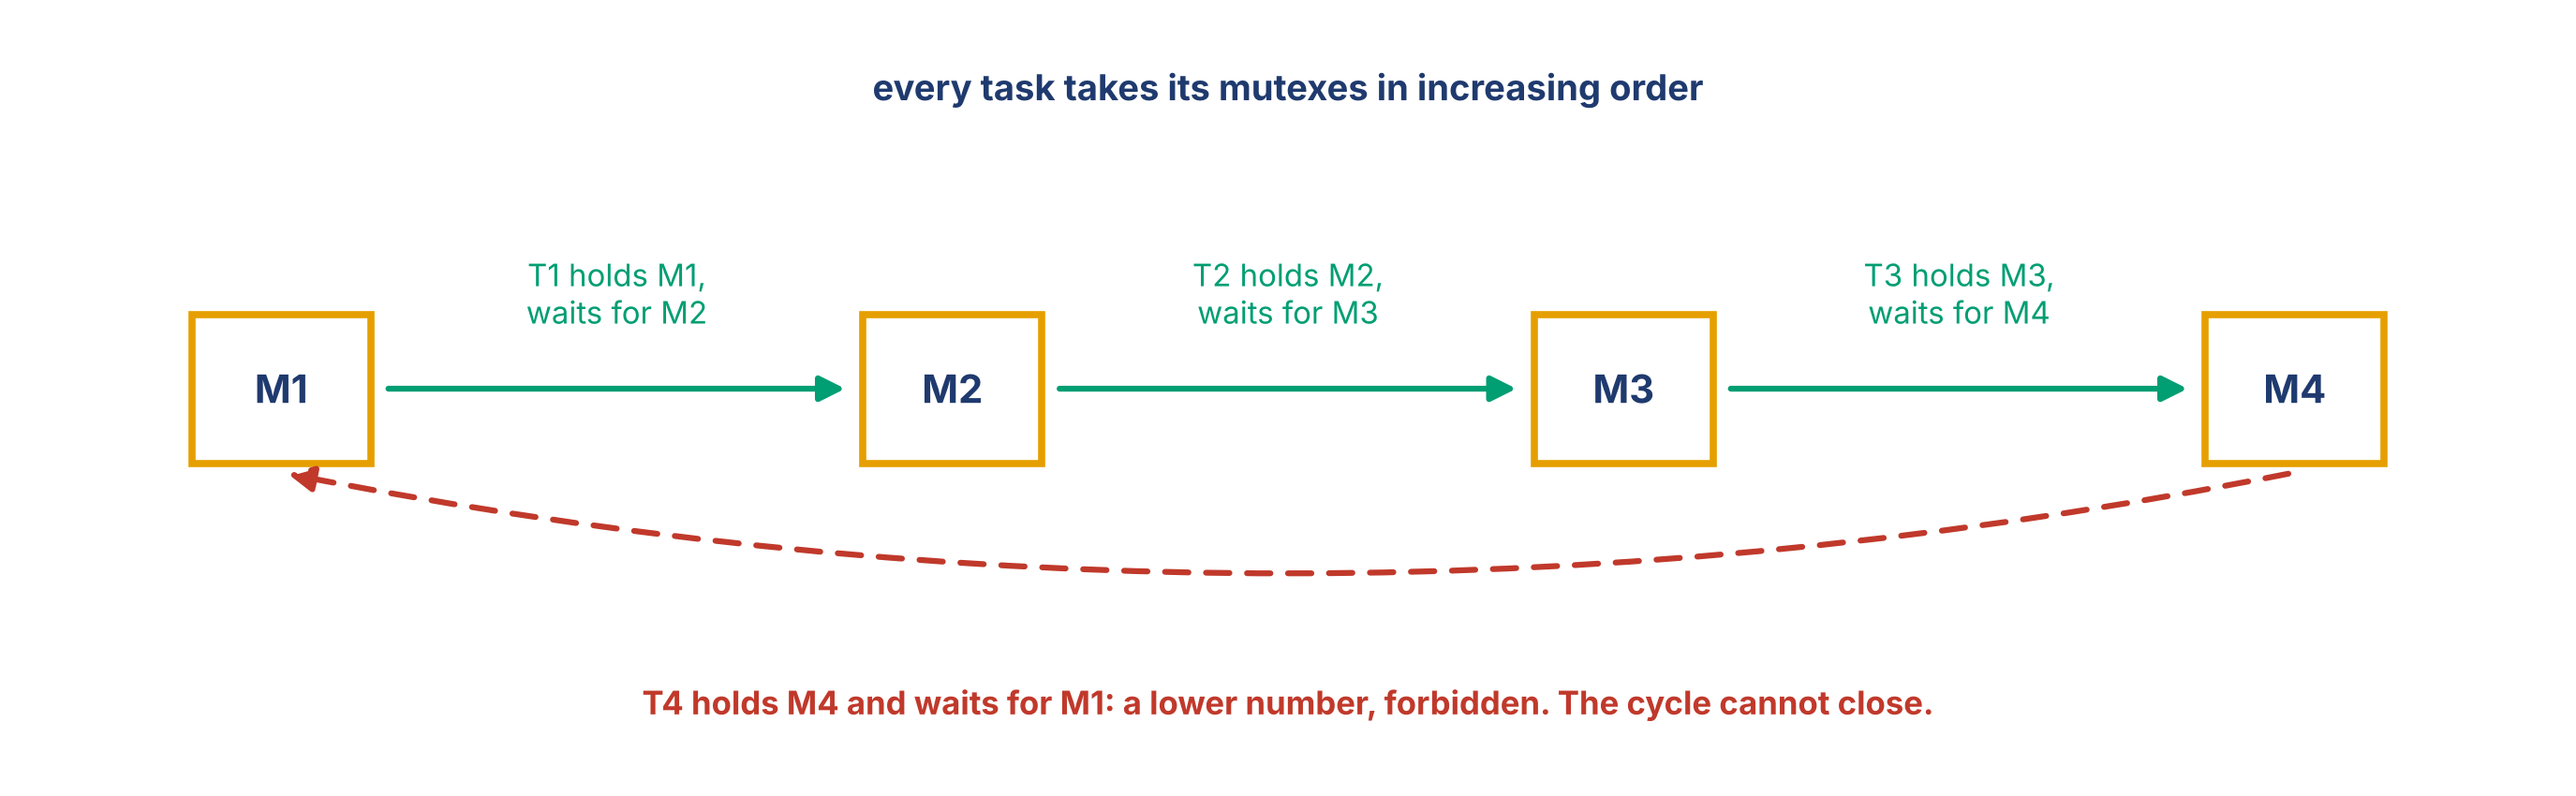
\includegraphics[width=0.75\textwidth]{contents/images/week-08/lock_ordering.png}
    \caption{Holding mutex $n$ and asking for $n+1$ respects the rule; closing the loop would need the holder of the last mutex to ask for the first one, which the rule forbids.}
\end{figure}
\emph{Why no cycle?} (``Try to explain it to your friends.'') Suppose a cycle: T1 holds Ma and waits for Mb, T2 holds Mb and waits for Mc, \dots, Tn holds Mz and waits for Ma. Each waits for a higher number, so $a < b < \dots < z < a$: impossible. In practice: number the mutexes, then check every task, what it holds and what it requests; a task that holds a higher number than the one it wants breaks the rule. A task that holds M2 and finds it also needs M1 must give back M2, take M1, take M2 again, and \textbf{check the data again}, because others may have changed it meanwhile. \emph{Is there a tool that checks this at compile time?} The professor knows none, though it is feasible.

\paragraph{Avoidance and detection: the ideas.}
\begin{itemize}
    \item \textbf{Avoidance}: programmers are free, and the OS refuses any lock that can lead to a deadlock. A task declares in advance the most it may ever ask; at each request the kernel checks whether, granting it, there is still an order in which all tasks can finish (a \textbf{safe} state); if not, the task waits even if the resource is free. The classic is the \textbf{banker's algorithm} (``I am not explaining it because I do not remember how it works, so it is not important''). Rare in small systems: maximums are hard to know, and a graph check at every lock is costly; FreeRTOS does not implement it.
    \item \textbf{Detection and recovery}: let it happen, and look from time to time. \emph{Detect}: build the graph of who waits for whom, and search for a cycle. \emph{Recover}: stop a task in the cycle or take a resource away; the hard part is the half-finished work. A simpler version is common: a task that watches whether the others still make \textbf{progress}. It does not prove a deadlock, only that nothing moves; you write one for the \texttt{deadlock} program.
\end{itemize}

\subsection{Dining philosophers}
(The professor's disclaimer: he finds this problem useless unless you like very abstract problems, but someone he respects told him an OS course cannot skip it; its solutions are a good way to think about avoiding deadlock.) Five philosophers sit at a round table, with \textbf{one fork} between each pair of neighbours. Each alternates thinking and eating, and to eat needs \textbf{two} forks, left and right, picked up one at a time. Each philosopher is a task, each fork a mutex. The first program: take the left fork, take the right one, eat, put both down, think. If all five take their left fork at once, every right fork is taken: all wait for ever.
\begin{figure}[H]
    \centering
    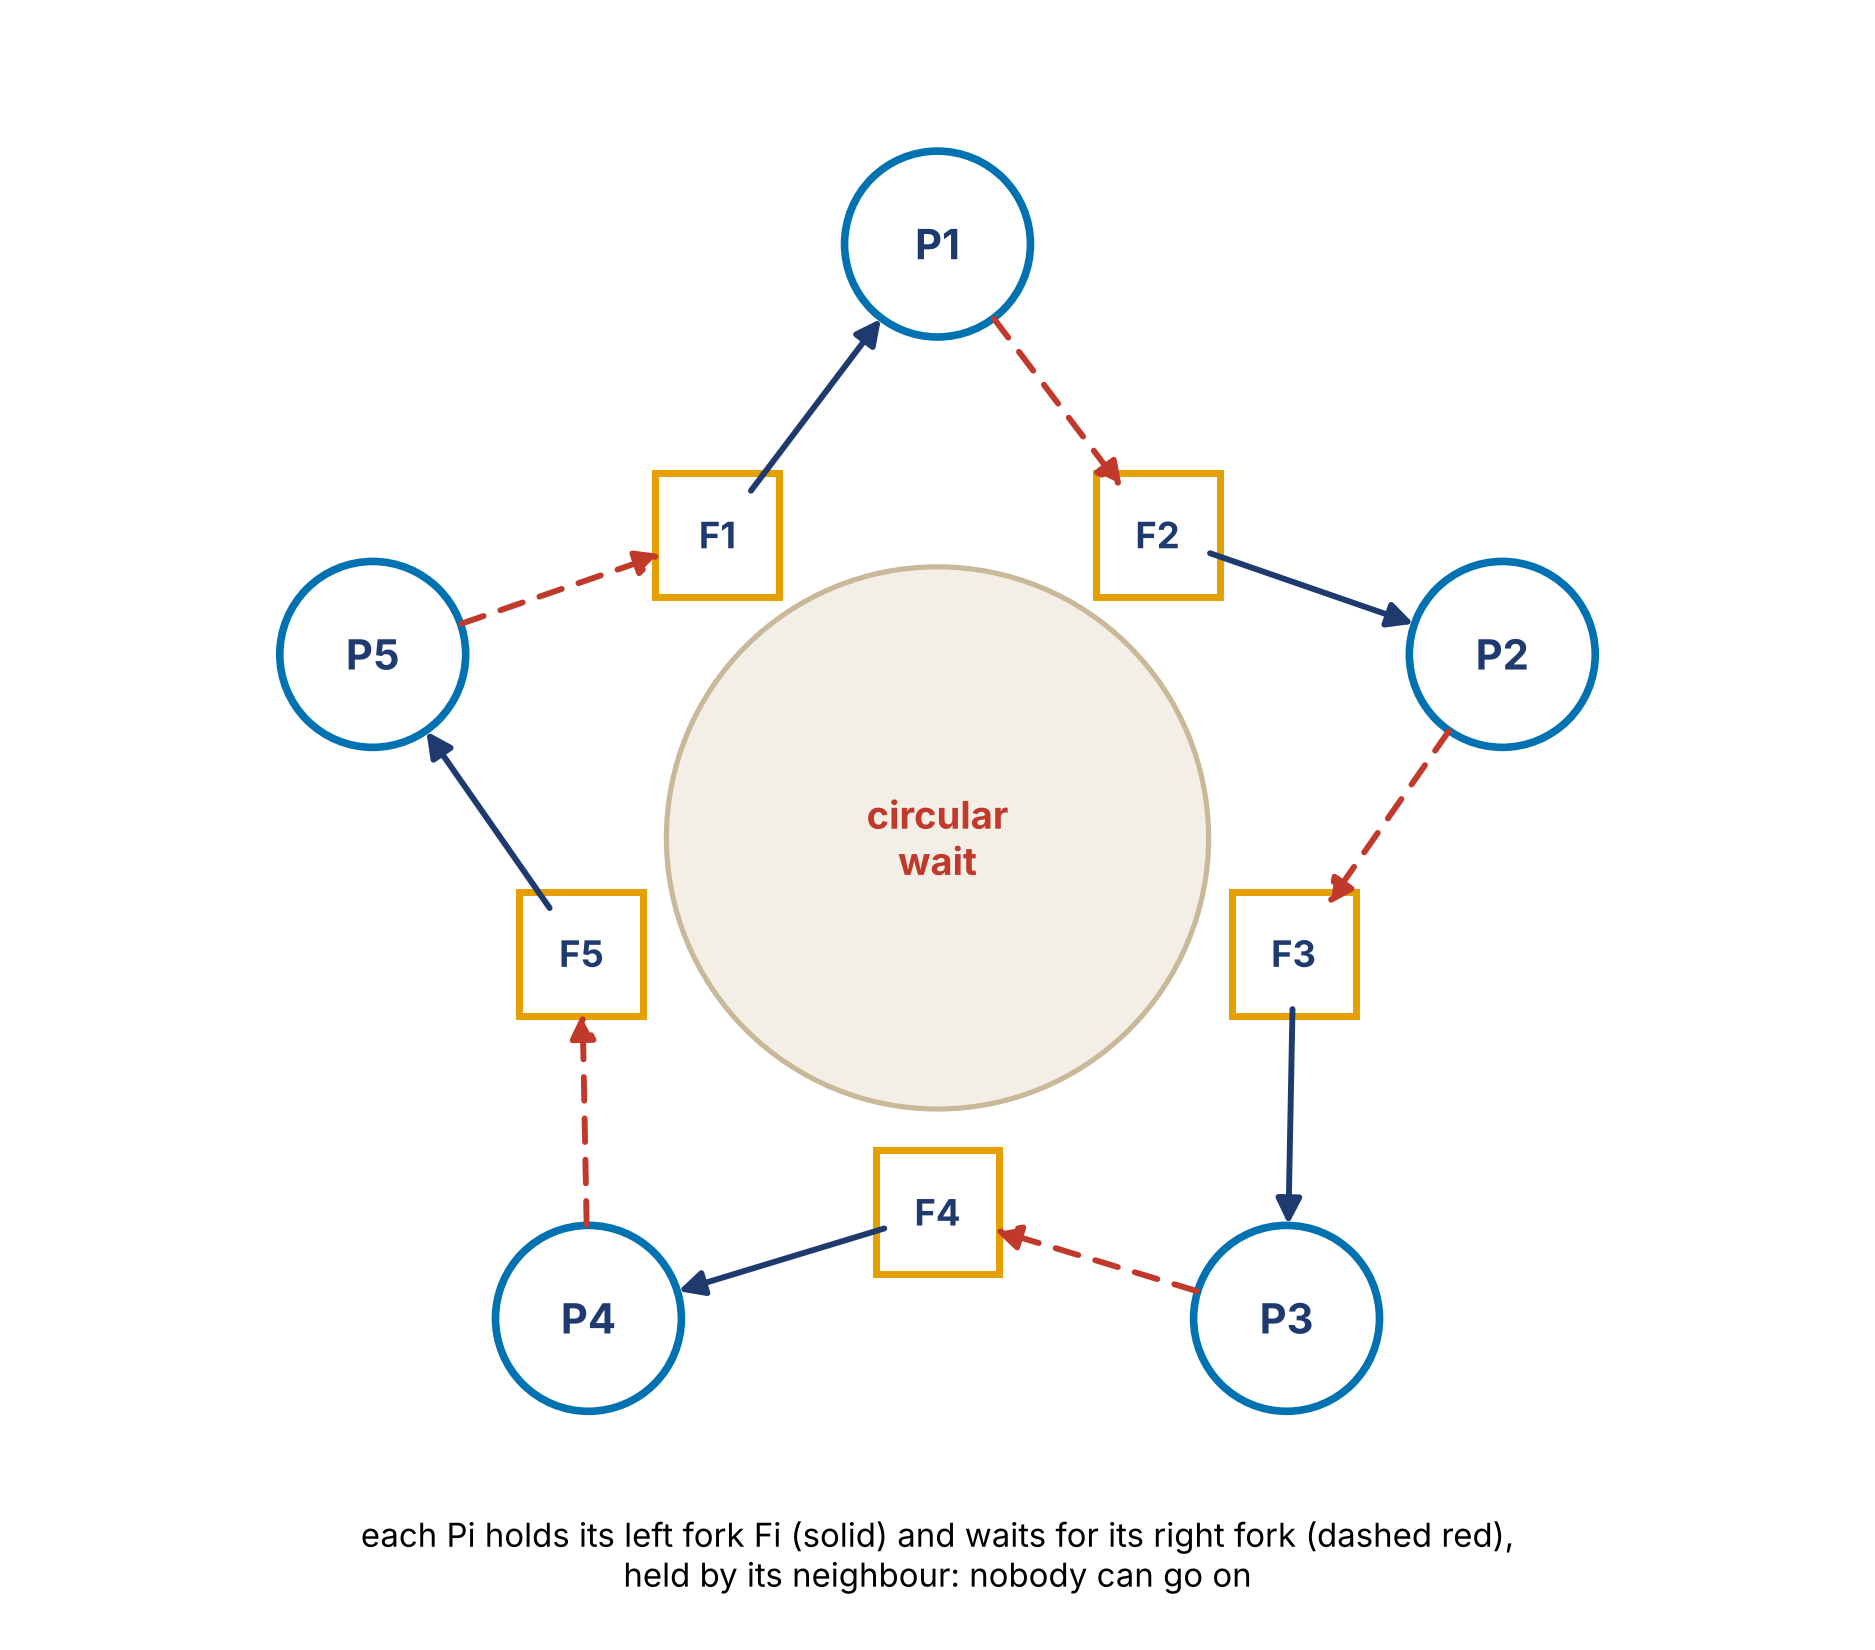
\includegraphics[width=0.5\textwidth]{contents/images/week-08/philosophers.png}
    \caption{The deadlock: P1 waits for F2, held by P2; P2 for F3; P3 for F4; P4 for F5; P5 for F1, held by P1.}
\end{figure}
\begin{lstlisting}[basicstyle=\ttfamily\footnotesize]
semaphore F1 = 1, F2 = 1, F3 = 1, F4 = 1, F5 = 1;

Pi:  for ever:  think;  wait( Fi );  wait( Fi+1 );  eat;  signal both;
\end{lstlisting}
(For P5, \texttt{Fi+1} is F1.) All four conditions hold. With only P1 to P4 at the table there is no deadlock: F5 stays free.

\paragraph{Try it on paper: fix the philosophers.} For each fix, say which condition it breaks.
\begin{enumerate}
    \item Forks are numbered. Each philosopher takes the \textbf{lower-numbered} of its two forks first. So P5 takes F1 first, and then F5.
    \item A counting semaphore with initial value 4 lets only \textbf{four} philosophers sit at the table at once.
    \item A philosopher picks up the two forks only if \textbf{both} are free, in one atomic step.
\end{enumerate}
\needspace{4\baselineskip}
\textbf{Solution.}
\begin{enumerate}
    \item \textbf{Circular wait}: lock ordering. P1 to P4 take F1 to F4; P5 must start with F1, already taken, so it holds nothing and waits. F5 is free, P4 eats and starts freeing forks, and finally P5 eats.
    \item \textbf{Circular wait} again, more drastic: ``only four can eat, one of you stays outside''. Five forks for four philosophers: at least one gets both.
    \item \textbf{Hold and wait}: nobody holds one fork while waiting for another.
\end{enumerate}
\begin{figure}[H]
    \centering
    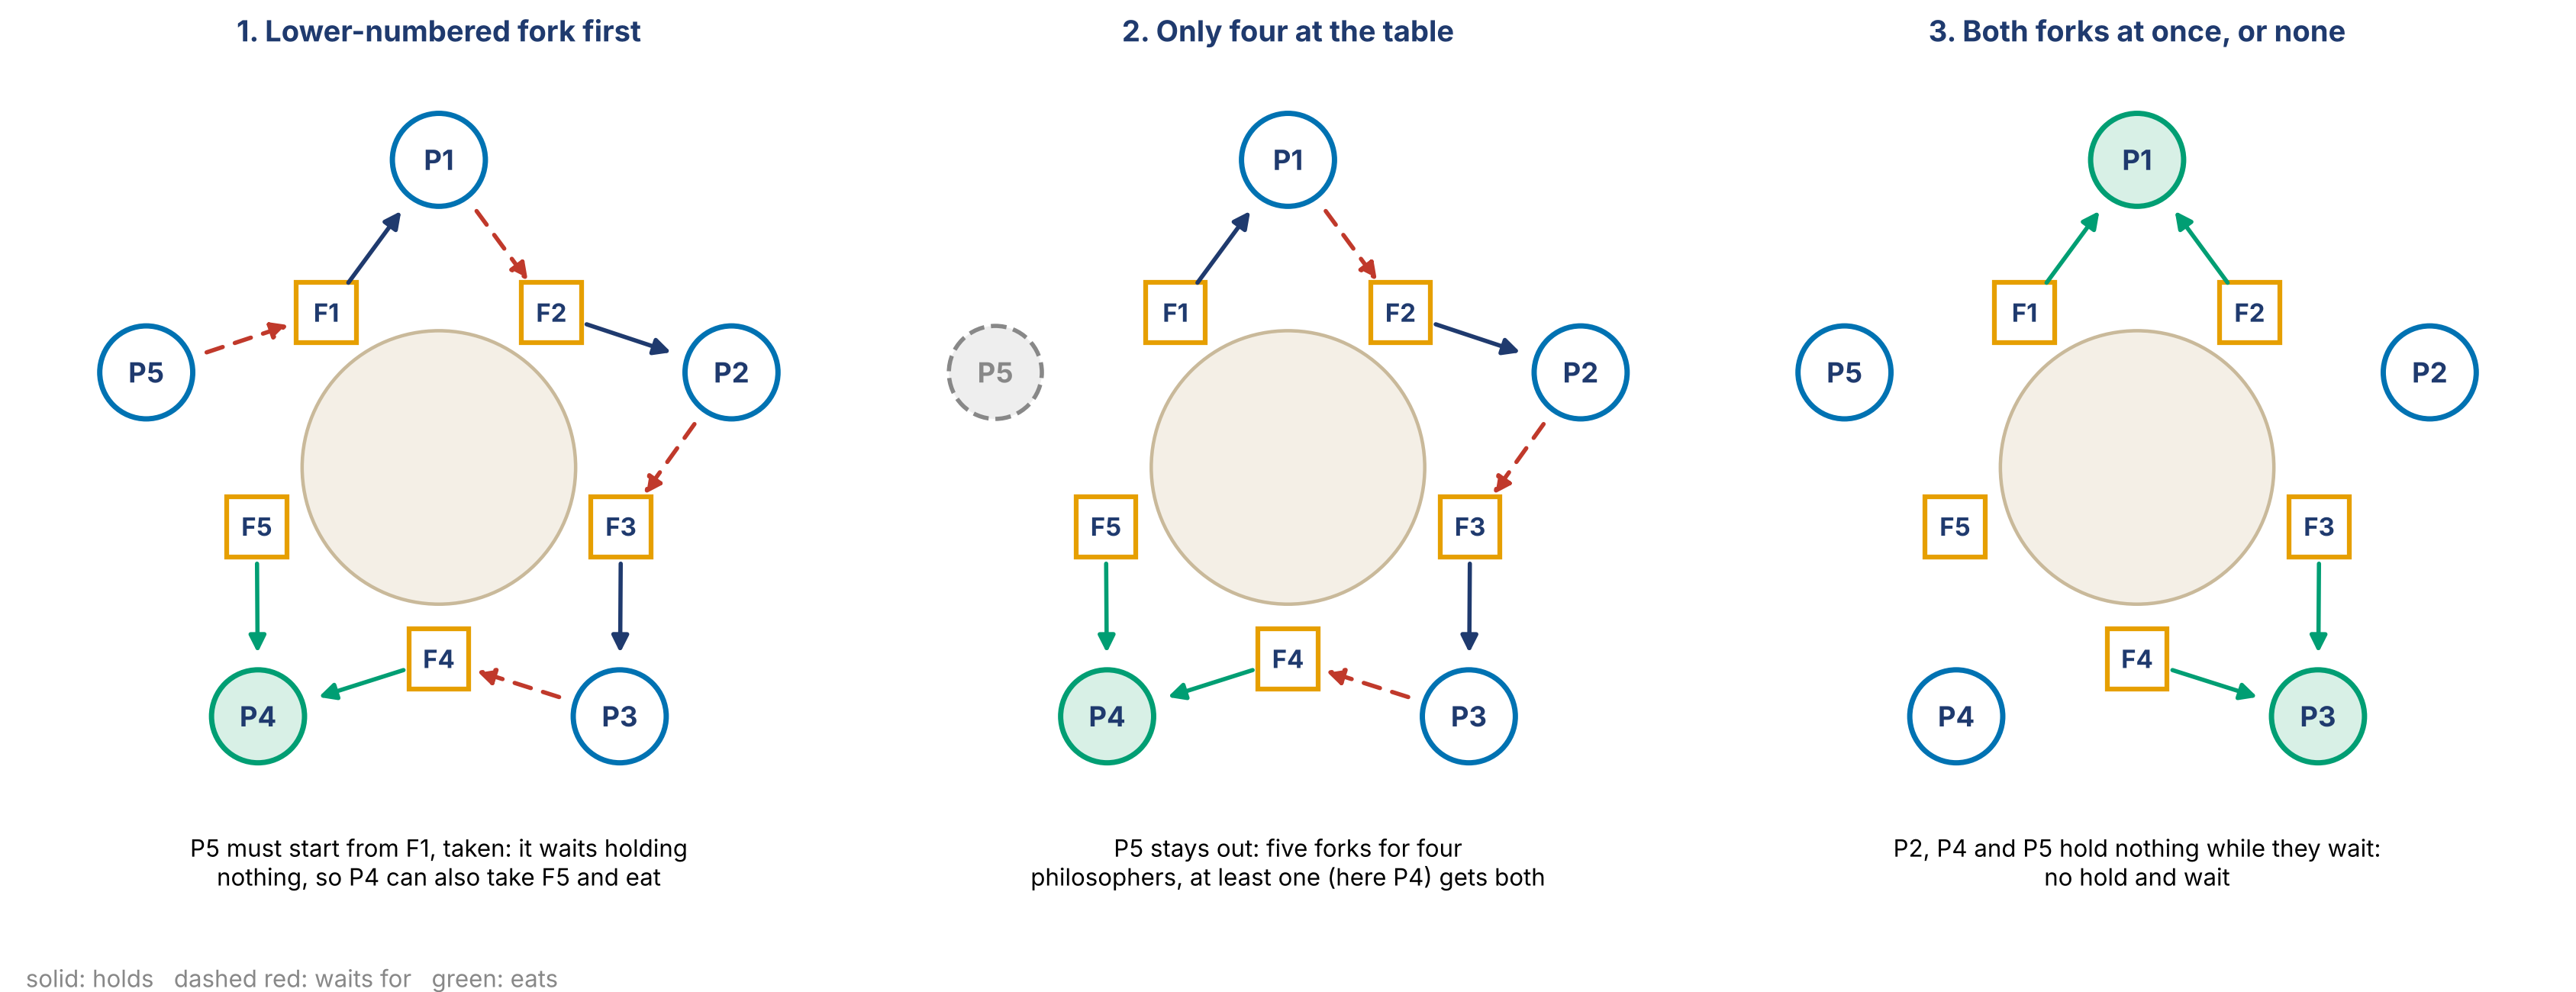
\includegraphics[width=1\textwidth]{contents/images/week-08/philosophers_fixes.png}
    \caption{The three fixes at the moment when, without them, all five would hold one fork: in each, the circle cannot close and somebody eats.}
\end{figure}
In class also ``the rule of the strongest'': one philosopher takes \textbf{two} forks, finishes, and the four left can always eat. Deadlock exercises are graphs on paper, so they are easy exam exercises.

\subsection{Message passing}
So far tasks shared \textbf{memory} (a shared variable) and protected it with synchronization primitives. The other model, used by many OSs, is \textbf{message passing}: tasks do not share a variable, they \textbf{communicate}, with two operations, \texttt{send( message )} and \texttt{receive( message )}. In FreeRTOS it needs no new primitive, but a different way of thinking about the program.
\begin{figure}[H]
    \centering
    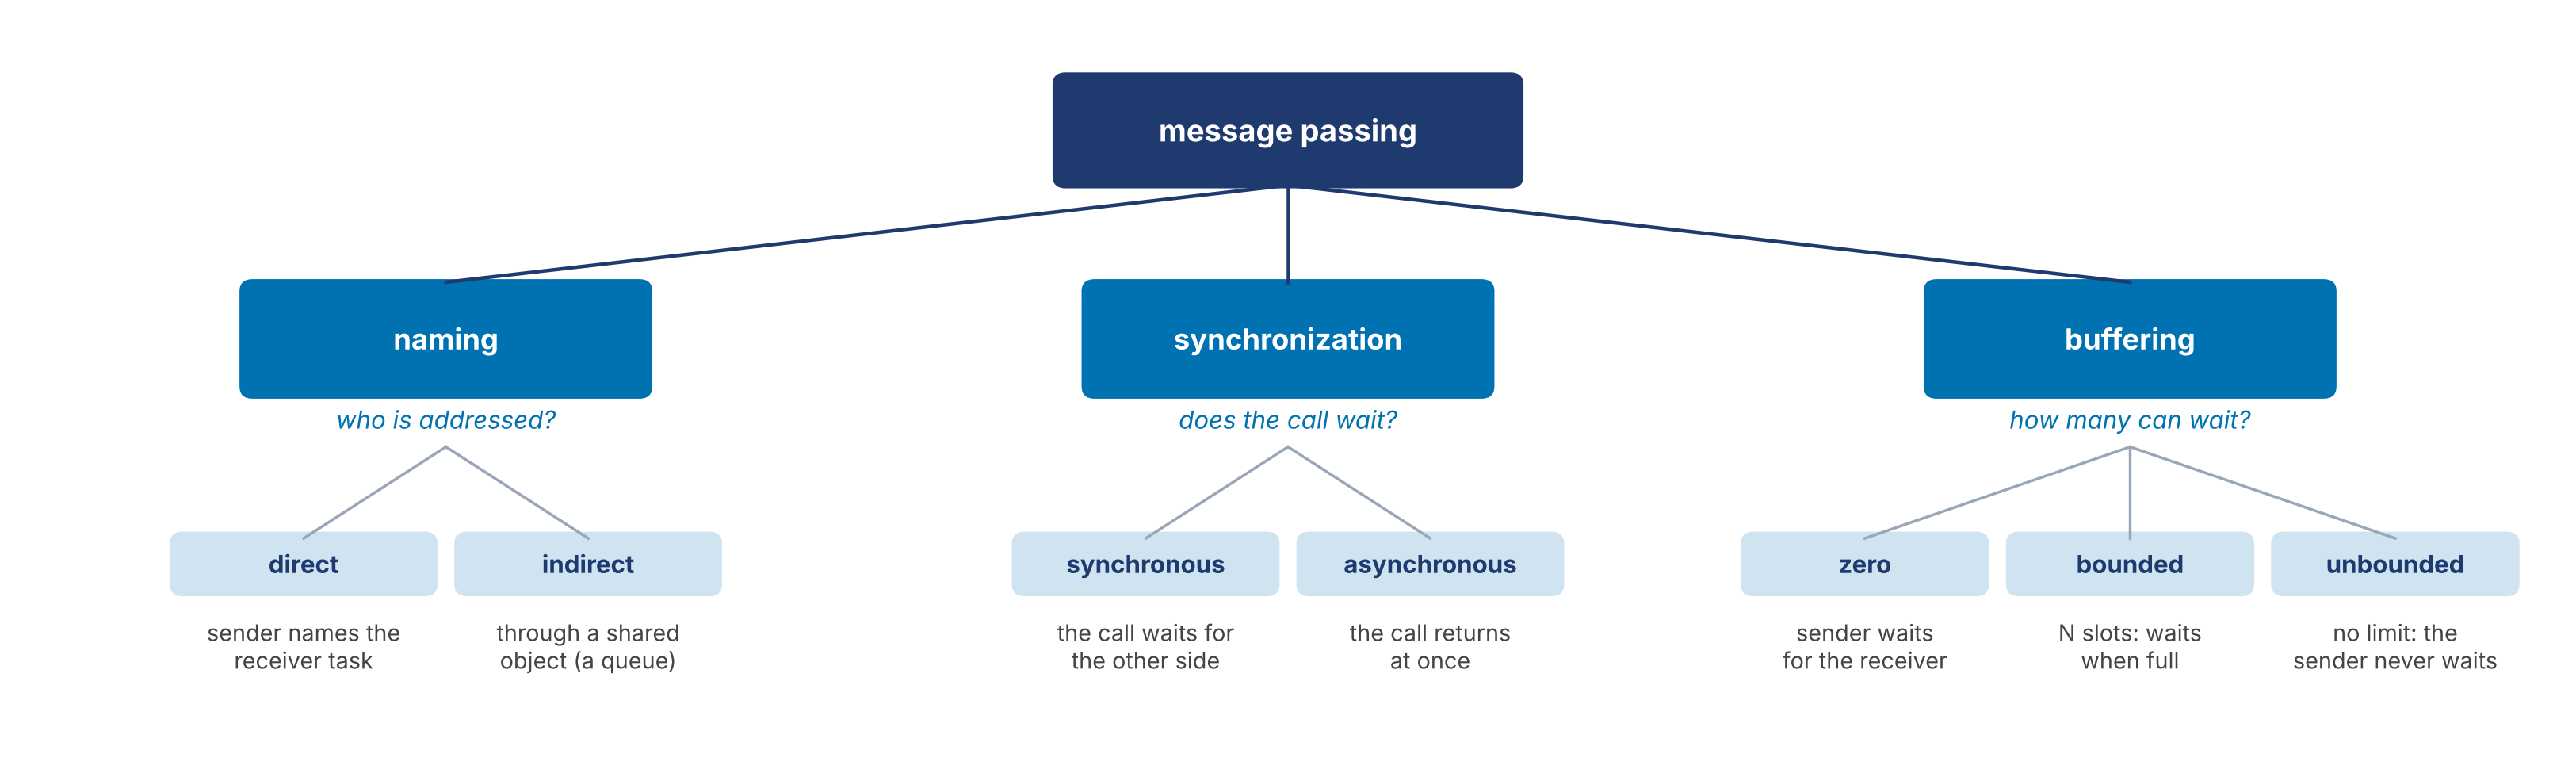
\includegraphics[width=1\textwidth]{contents/images/week-08/message_passing_tree.png}
    \caption{The three questions that every message-passing system answers. Your gatekeeper is one possible set of answers.}
\end{figure}

\paragraph{Naming: who is addressed?}
\begin{itemize}
    \item \textbf{Direct}: \texttt{send( T2, m )}, \texttt{receive( T1, m )}. Tasks name each other, and the OS routes the message. Simple, but changing a task means changing all those that name it.
    \item \textbf{Indirect}: \texttt{send( Q, m )}, \texttt{receive( Q, m )}. Tasks name an object in between, a \textbf{mailbox}, a fixed connection (a FreeRTOS queue is one). The sender does not know who receives, and several tasks can send or receive.
\end{itemize}
\emph{Which is more costly?} (A poll; most said direct.) A trade-off: direct needs a \textbf{router} in the OS, which costs algorithm and CPU time; indirect needs \textbf{one connection per pair} that talks, which costs objects. Three tasks are easy either way; a hundred tasks talking means far too many queues.

\paragraph{Synchronization: does the call wait?}
\begin{itemize}
    \item \textbf{Synchronous} (blocking): \texttt{send} waits until the receiver has the message, or \texttt{receive} until a message arrives; the waiting task uses no CPU.
    \item \textbf{Asynchronous} (non-blocking): the call returns \textbf{at once}, whether or not the operation could complete.
    \item If both wait for each other, the tasks meet at the same point: a \textbf{rendezvous}.
\end{itemize}
\emph{Which do you like more?} (A student: synchronous, more predictable.) Not really: synchronous wastes no CPU but you do not know when you will wake up; asynchronous never waits, but try-fail-try is close to \textbf{polling}, which wastes CPU. ``I like both of them, and I don't like both of them'': in operating systems \textbf{nothing is perfect, it is always a trade-off}.

\paragraph{Buffering: how many messages can wait?}
\begin{itemize}
    \item \textbf{Zero}: no slots. The sender waits until the receiver takes the message: always a rendezvous. No memory, but every send that finds the channel busy waits or fails.
    \item \textbf{Bounded}: N slots; the sender waits only when all are full. The middle ground.
    \item \textbf{Unbounded}: the sender never waits. ``The solution for dreamers'': memory is finite, so it is only a model; really, it means the OS, not the programmer, chooses the size.
\end{itemize}

\paragraph{Where FreeRTOS fits.} Message passing is the \textbf{queue}: no task names, no routing, a connection among the tasks that share it. \emph{With several receivers, who gets the message?} (An exam question type.) The \textbf{scheduler} decides: the first receiver that runs. The timeout makes it blocking or not; the length makes it bounded\footnote{In class: ``zero or bounded, but not unlimited''. A true zero-slot queue is not what \texttt{xQueueCreate} gives (its length is at least 1); a queue of length 1 with a blocking send is the closest thing to a rendezvous.}.
\begin{enumerate}
    \item \texttt{xQueueSend( q, \&m, portMAX\_DELAY )}, on a queue of length 8: \textbf{indirect, bounded, blocking when full}; if there is room, it returns without meeting the receiver.
    \item \texttt{xQueueSend( q, \&m, 0 )}, on the same queue: \textbf{indirect, bounded, asynchronous}; on a full queue it returns \texttt{errQUEUE\_FULL}, and the task decides.
    \item Two tasks, each blocked in \texttt{xQueueSend} on a full queue that only the other one reads, are in \textbf{deadlock}. Messages remove shared variables, \textbf{not deadlocks}.
\end{enumerate}

\paragraph{Shared memory or messages?} The question of the \textbf{second part of the exam}: an application always shares something. There, efficiency matters less than \textbf{simplicity}: less code, easier to write.
\begin{center}
\small
\begin{tabular}{P{0.17} P{0.34} P{0.38}}
    \hline
    & \textbf{shared memory with locks} & \textbf{message passing through a queue} \\
    \hline
    data & one copy, used in place & copied in and out \\
    cost & little: a take and a give & two copies per message \\
    large data & fine & slow if copied; sending a pointer brings back the sharing \\
    who protects it & every task must remember the lock & the kernel and the owner task \\
    typical bug & forgotten lock, race, deadlock & full queue, lost messages, deadlock \\
    \hline
\end{tabular}
\end{center}
The first rows say ``shared memory'': a shared counter is a global with a mutex, while with messages every task would work on a local copy and send updates. The point for messages: protecting shared data is \textbf{your} responsibility, and a wrong or forgotten wait breaks the program; with messages the \textbf{kernel} protects, and tasks are more \textbf{isolated}. \textbf{Small messages between tasks: a queue. Large data used in place: a mutex, with a clear lock order.} There is no strict rule (``I'm sorry''): every problem can be solved both ways.

\subsection{Try it: two tasks and two mutexes}
\textbf{Requirement}: two workers use two mutexes, M1 and M2, in \textbf{opposite orders}: W1 takes M1 then M2, W2 takes M2 then M1. Given in \texttt{apps/deadlock.c}: the counters \texttt{progress1} and \texttt{progress2}, the timings \texttt{PAUSE\_TICKS}, \texttt{JOB\_TICKS}, \texttt{REST\_TICKS}, and \texttt{print\_task\_table}. The mutexes are global but \textbf{not} \texttt{static}, because the optional debugger session looks at them.
\par\noindent\begin{minipage}[t]{0.42\textwidth}
\begin{lstlisting}[language=C, showstringspaces=false, basicstyle=\ttfamily\scriptsize]
/* outside the functions */
SemaphoreHandle_t xMutex1;
SemaphoreHandle_t xMutex2;

/* main */
xMutex1 = xSemaphoreCreateMutex();
xMutex2 = xSemaphoreCreateMutex();
\end{lstlisting}
\end{minipage}\hfill
\begin{minipage}[t]{0.55\textwidth}
\begin{lstlisting}[language=C, showstringspaces=false, basicstyle=\ttfamily\scriptsize]
/* vWorker1 (vWorker2: M2 first, then M1) */
for( ;; )
{
    xSemaphoreTake( xMutex1, portMAX_DELAY );
    vTaskDelay( PAUSE_TICKS );
    xSemaphoreTake( xMutex2, portMAX_DELAY );
    vTaskDelay( JOB_TICKS );
    progress1++;
    xSemaphoreGive( xMutex2 );
    xSemaphoreGive( xMutex1 );
    vTaskDelay( REST_TICKS );
}
\end{lstlisting}
\end{minipage}

\noindent Run \texttt{make APP=deadlock run}: only the banner appears. A deadlock prints no error, and a program that works in silence looks the same: we need a task that \textbf{watches} the others.

\subsection{Try it: a task that watches the others}
The last thing shown in class: \textbf{detection}. A small \textbf{monitor} checks whether the other tasks make \textbf{progress}. It needs \textbf{instrumentation}: one variable per task (\texttt{progress1}, \texttt{progress2}, \texttt{volatile} because another task changes them), incremented at every loop. The monitor is last week's periodic template, with a period of 100 ticks (one second): it compares the counters with their old values, and if none moved it is a \textbf{potential} deadlock: it prints the task table and the holder of each mutex.
\begin{lstlisting}[language=C, showstringspaces=false, basicstyle=\ttfamily\scriptsize]
/* vMonitor */
unsigned long last1 = 0;
unsigned long last2 = 0;
TickType_t wake = xTaskGetTickCount();

for( ;; )
{
    vTaskDelayUntil( &wake, 100 );
    console_print( "MON: tick %lu, W1 = %lu, W2 = %lu\n",
                   ( unsigned long ) wake, progress1, progress2 );

    if( progress1 == last1 && progress2 == last2 )
    {
        console_print( "MON: no progress in the last second, tasks:\n" );
        print_task_table();
        console_print( "MON: M1 held by %s, M2 held by %s\n",
                       holder_name( xMutex1 ), holder_name( xMutex2 ) );
    }

    last1 = progress1;
    last2 = progress2;
}
\end{lstlisting}
The last print gives what the table cannot: who holds each mutex. \texttt{holder\_name}, above \texttt{vMonitor}:
\begin{lstlisting}[language=C, showstringspaces=false, basicstyle=\ttfamily\scriptsize]
static const char * holder_name( SemaphoreHandle_t mutex )
{
    TaskHandle_t holder = xSemaphoreGetMutexHolder( mutex );

    return ( holder != NULL ) ? pcTaskGetName( holder ) : "nobody";
}
\end{lstlisting}
\texttt{xSemaphoreGetMutexHolder} returns the holder of a mutex, or \texttt{NULL} if it is free (it needs \texttt{INCLUDE\_xSemaphoreGetMutexHolder}). \texttt{pcTaskGetName} returns the name given in \texttt{xTaskCreate}; given \texttt{NULL} it would return the caller's name, so we test first.

\noindent \texttt{print\_task\_table} is given because it is only text handling: it calls \texttt{vTaskList} on a \texttt{static} buffer (a task stack is small) and prints line by line (\texttt{console\_print} cuts long lines). After about 4 seconds:
{\verbatimscriptsize
\begin{verbatim}
deadlock: W1 takes M1 then M2, W2 takes M2 then M1
MON: tick 100, W1 = 0, W2 = 0
MON: no progress in the last second, tasks:
  MON                  X          3           368         3
  IDLE                 R          0           237         4
  W2                   B          1           221         2
  W1                   B          1           221         1
MON: M1 held by W1, M2 held by W2
MON: tick 200, W1 = 0, W2 = 0
...
\end{verbatim}}
\begin{itemize}
    \item Both counters stay at 0. \texttt{PAUSE\_TICKS} makes it happen every time: W1 holds M1 and sleeps one tick, so W2 takes M2; at tick 1 both wake up, each asks for the mutex the other holds, and both block for good. The program did not crash, and the monitor still runs.
    \item The holder line gives two edges of the graph, M1 $\rightarrow$ W1 and M2 $\rightarrow$ W2; with the code, each worker waits for the other mutex: the picture of the RAG section, with T1 $=$ W1 and T2 $=$ W2.
\end{itemize}

\paragraph{Reading the \texttt{vTaskList} table.} \texttt{vTaskList} returns information on all tasks: not for functionality, but very nice for \textbf{debugging} (``print-f is still the best debugger''; gdb is powerful but not user-friendly). A task with 0 free stack, for example, has a stack too small. One line per task, with tabs and no title; the line \texttt{W2 B 1 221 2}:
\begin{center}
\small
\begin{tabular}{l c P{0.6}}
    \hline
    \textbf{column} & \textbf{here} & \textbf{meaning} \\
    \hline
    name & W2 & the name given in \texttt{xTaskCreate}, followed by spaces \\
    state & B & X running, R ready, B blocked, S suspended, D deleted \\
    priority & 1 & the current priority \\
    free stack & 221 & the smallest free stack so far, in \textbf{words} (not bytes) \\
    number & 2 & given by creation order \\
    \hline
\end{tabular}
\end{center}
MON is X, because it calls \texttt{vTaskList}; IDLE is R; W1 and W2 stay B, and may swap lines (the order follows the kernel's lists). A task waiting with \texttt{portMAX\_DELAY} really sits on the \textbf{suspended} list, but is shown as B: \texttt{vTaskGetInfo} reports as blocked a task that also has its \texttt{xEventListItem} on a wait list. A task parked with \texttt{vTaskSuspend( NULL )} is S.

\paragraph{What the monitor tells us.}
\begin{itemize}
    \item It has a \textbf{higher priority} than the workers (3 against 1), so it runs even if a worker never blocks: a worker stuck in a busy loop would starve a monitor below it.
    \item ``No progress'' does \textbf{not prove} a deadlock: a very long job, a starved task, or a wait for external events give the same counters; B for both is stronger evidence, but could be a long delay. How many silent rounds before declaring a deadlock is a choice, because recovery (\textbf{killing and restarting} tasks) costs a lot.
    \item It misses the \textbf{request edges}: \texttt{vTaskList} says B, not on what, and FreeRTOS has no call that returns the waiters of a mutex. The kernel has them in the wait lists, and the debugger can read them.
\end{itemize}

\subsection{Who holds what: the debugger (optional)}
To \textbf{prove} the deadlock you also need the request edges, which are in the kernel objects: in this port gdb can read every kernel variable. A session to do at home, as last week's.
\begin{itemize}
    \item \textbf{Start}: in the solution folder (or in your base once the workers are written) run \texttt{make APP=deadlock debug}: QEMU starts frozen and waits for gdb on port 1234. In a second terminal, in the same folder: \texttt{arm-none-eabi-gdb build/deadlock.elf} (on Linux: \texttt{gdb-multiarch}).
    \item \textbf{Break by function name, not by line number}: a line number changes as soon as anyone edits the file, and your \texttt{deadlock.c} is not the solution's. \texttt{vTaskList} is called in one place only, in \texttt{print\_task\_table}, right after the \texttt{no progress} message: so this breakpoint stops exactly when the monitor has detected the stall, with \texttt{MON: no progress in the last second, tasks:} as the last line in the QEMU terminal, and the table not printed yet.
    \item Below, the source lines gdb prints at a stop are left out (they change with the kernel version); your addresses may differ, the names will not. Long commands are split with a final \texttt{\textbackslash}, a gdb line continuation.
\end{itemize}
{\verbatimscriptsize
\begin{verbatim}
(gdb) target remote :1234                  # step 1: connect, stop at the stall
(gdb) break vTaskList
(gdb) continue
Breakpoint 1, vTaskList (pcWriteBuffer=0x20000070 <list> "") at ../../FreeRTOS/Source/tasks.c

(gdb) print pxCurrentTCB                   # step 2: who is running?
$1 = (TCB_t * volatile) 0x20002038 <ucHeap+4556>
(gdb) print pxCurrentTCB->pcTaskName
$2 = "MON\000\000\000\000\000\000"

                                           # step 3: who holds each mutex?
(gdb) print ((TCB_t *) ((struct QueueDefinition *) xMutex1)\
             ->u.xSemaphore.xMutexHolder)->pcTaskName
$4 = "W1\000\000\000\000\000\000\000"
(gdb) print ((TCB_t *) ((struct QueueDefinition *) xMutex2)\
             ->u.xSemaphore.xMutexHolder)->pcTaskName
$6 = "W2\000\000\000\000\000\000\000"

(gdb) print progress1                      # step 4: the counters
$7 = 0
(gdb) print progress2
$8 = 0

                                           # step 5: the counts and the wait lists
(gdb) print ((struct QueueDefinition *) xMutex1)->uxMessagesWaiting
$9 = 0
(gdb) print ((TCB_t *) ((struct QueueDefinition *) xMutex1)\
             ->xTasksWaitingToReceive.xListEnd.pxNext->pvOwner)->pcTaskName
$11 = "W2\000\000\000\000\000\000\000"
(gdb) print ((TCB_t *) ((struct QueueDefinition *) xMutex2)\
             ->xTasksWaitingToReceive.xListEnd.pxNext->pvOwner)->pcTaskName
$12 = "W1\000\000\000\000\000\000\000"

(gdb) kill                                 # step 6: ends the session and QEMU (answer y)
\end{verbatim}}
\begin{itemize}
    \item \textbf{Step 2}: the running task is the monitor, as expected. The address of its TCB falls inside \texttt{ucHeap}, the kernel's heap (\texttt{portable/\allowbreak MemMang/\allowbreak heap\_4.c}): \texttt{xTaskCreate} takes the TCB from there.
    \item \textbf{Step 3}: a handle has a type that hides the content of the object, so we tell gdb what it really points to, \texttt{struct QueueDefinition}, the \texttt{Queue\_t} of Unit 2. The holder (\texttt{u.xSemaphore.xMutexHolder}, printed alone it is an address such as \texttt{0x20001348}) is a task handle, that is the address of a TCB, so we cast it to \texttt{TCB\_t *} and read the name. \textbf{W1 holds M1, W2 holds M2}: the two assignment edges.
    \item \textbf{Step 5}: a mutex is a queue of length 1, so a count of 0 means it is taken. The head of its \texttt{xTasksWaitingToReceive} is the task that waits for it; in a list, \texttt{xListEnd.pxNext} is the first item, and the \texttt{pvOwner} of an item is its TCB. \textbf{W2 waits for M1, W1 waits for M2}: the two request edges.
\end{itemize}
Put together: W1 holds M1 and waits for M2, W2 holds M2 and waits for M1. This is exactly the resource-allocation graph, with T1 $=$ W1 and T2 $=$ W2: the cycle is now \textbf{proved from the kernel's own data}, which neither the counters nor the table could do.

\subsection{Try it: fix 1, the same order for everyone}
\textbf{Requirement}: with \texttt{DEMO=ordered}, W2 takes M1 first too (lock ordering), so the cycle cannot close. In \texttt{vWorker2}:
\begin{lstlisting}[language=C, showstringspaces=false, basicstyle=\ttfamily\footnotesize]
#ifdef DEMO_ORDERED
        xSemaphoreTake( xMutex1, portMAX_DELAY );
        vTaskDelay( PAUSE_TICKS );
        xSemaphoreTake( xMutex2, portMAX_DELAY );
#else
        /* the same three lines, with xMutex2 first */
#endif
\end{lstlisting}
{\verbatimscriptsize
\begin{verbatim}
deadlock: DEMO=ordered, both workers take M1 then M2
MON: tick 100, W1 = 9, W2 = 8
MON: tick 200, W1 = 17, W2 = 17
MON: tick 300, W1 = 25, W2 = 25
\end{verbatim}}
\begin{itemize}
    \item The counters keep rising, and the table is never printed. A round lasts about 12 ticks (1 pause, 1 job, 10 rest), so about 8 rounds per second (figure below).
    \item If W1 has M1, W2 waits for M1 \textbf{holding nothing}: W1 gets M2, finishes and gives both back. Hold and wait still happens, but the \textbf{circular wait} cannot: nobody holding M2 asks for M1.
    \item The release order does not matter, because a give never blocks: only the order of the \textbf{takes} counts.
    \item No run-time cost, but the rule must hold in \textbf{all} the code that takes these mutexes: one function written the other way brings the deadlock back.
\end{itemize}
\begin{figure}[H]
    \centering
    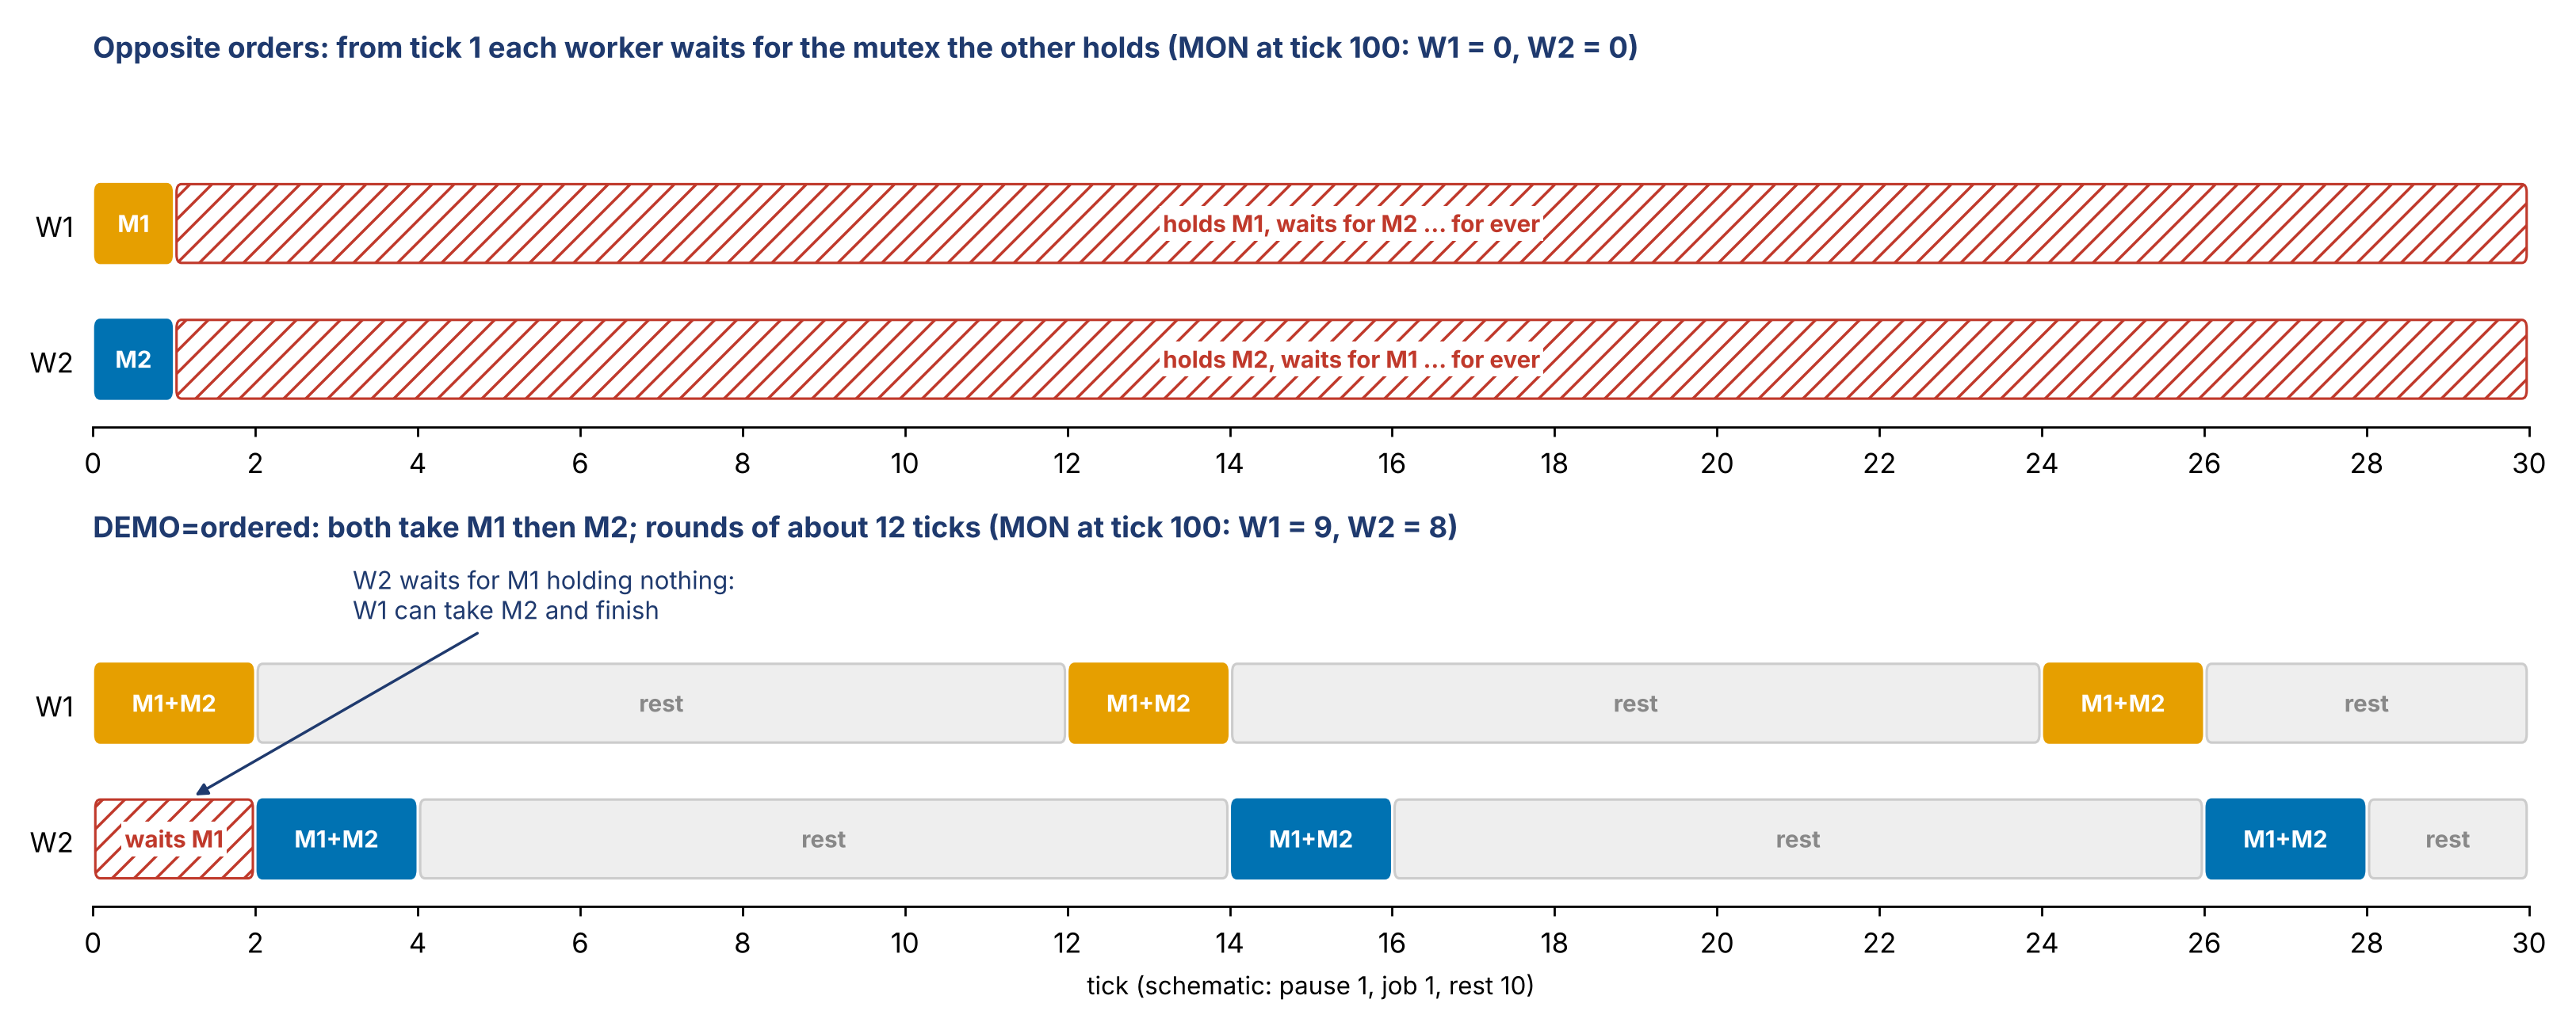
\includegraphics[width=1\textwidth]{contents/images/week-08/deadlock_two_runs.png}
    \caption{The two runs side by side, schematic. Above, opposite orders: both workers hold one mutex from tick 0 and wait for the other from tick 1, for ever. Below, \texttt{DEMO=ordered}: W2 waits for M1 holding nothing, so W1 finishes and the rounds go on.}
\end{figure}

\subsection{Try it: fix 2, give up after a while}
\textbf{Requirement}: with \texttt{DEMO=timeout}, the opposite orders stay, but no worker waits for ever for its \textbf{second} mutex: after 30 ticks it gives back the first one, sleeps, and retries. Each worker runs \texttt{worker\_round} in its loop, with its order and its back-off (W1: M1, M2, 7 ticks; W2: M2, M1, 13 ticks); the \texttt{continue} skips the old body.
\par\noindent\begin{minipage}[t]{0.6\textwidth}
\begin{lstlisting}[language=C, showstringspaces=false, basicstyle=\ttfamily\scriptsize]
#ifdef DEMO_TIMEOUT
#define WAIT_TICKS 30    /* at most 300 ms */

static void worker_round( const char * name,
    SemaphoreHandle_t first, SemaphoreHandle_t second,
    TickType_t backoff, volatile unsigned long * progress )
{
    xSemaphoreTake( first, portMAX_DELAY );
    vTaskDelay( PAUSE_TICKS );
    if( xSemaphoreTake( second, WAIT_TICKS ) == pdTRUE )
    {
        vTaskDelay( JOB_TICKS );
        ( *progress )++;
        xSemaphoreGive( second );
        xSemaphoreGive( first );
        vTaskDelay( REST_TICKS );
    }
    else
    {
        console_print( "%s: timeout at tick %lu,"
            " gives back and retries\n", name,
            ( unsigned long ) xTaskGetTickCount() );
        xSemaphoreGive( first );
        vTaskDelay( backoff );
    }
}
#endif
\end{lstlisting}
\end{minipage}\hfill
\begin{minipage}[t]{0.37\textwidth}
\begin{lstlisting}[language=C, showstringspaces=false, basicstyle=\ttfamily\scriptsize]
/* vWorker1, first in the loop */
#ifdef DEMO_TIMEOUT
    worker_round( "W1", xMutex1,
                  xMutex2, 7,
                  &progress1 );
    continue;
#endif

/* vWorker2, first in the loop */
#ifdef DEMO_TIMEOUT
    worker_round( "W2", xMutex2,
                  xMutex1, 13,
                  &progress2 );
    continue;
#endif
\end{lstlisting}
\end{minipage}

\noindent The first take may still wait for ever: the task holds nothing then, so it blocks nobody. The failure branch does not give the mutex it did not get (Unit 2). The solution has the same logic in one function, \texttt{vWorker}, with the values in a \texttt{worker\_t} passed as the task parameter.
{\verbatimscriptsize
\begin{verbatim}
deadlock: DEMO=timeout, second mutex taken with a timeout
W1: timeout at tick 31, gives back and retries
MON: tick 100, W1 = 5, W2 = 6
MON: tick 200, W1 = 14, W2 = 14
MON: tick 300, W1 = 22, W2 = 23
\end{verbatim}}
\begin{figure}[H]
    \centering
    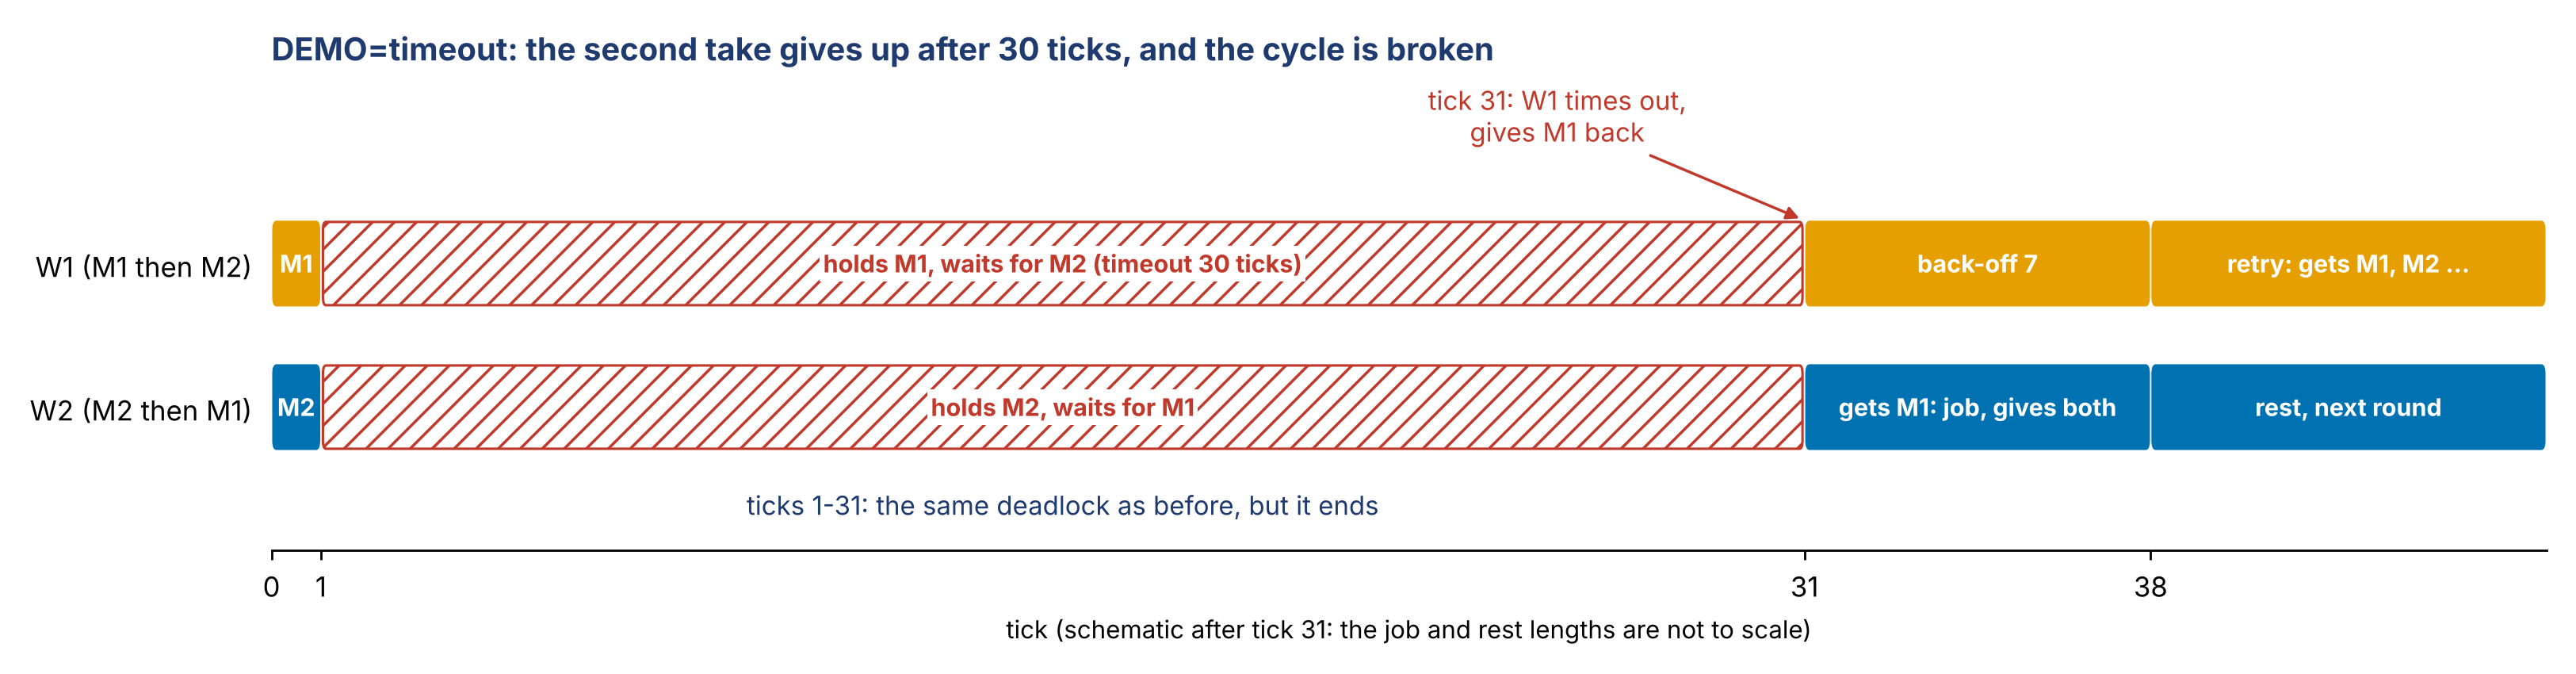
\includegraphics[width=1\textwidth]{contents/images/week-08/deadlock_timeout.png}
    \caption{The start of the \texttt{DEMO=timeout} run: the same deadlock as before from tick 1, until W1's timeout at tick 31.}
\end{figure}
\begin{itemize}
    \item \textbf{One timeout}: at tick 1 the same deadlock as before; at tick 31 W1 gives M1 back, W2 gets it and finishes. \textbf{Not two}: W2's 30 ticks also end at tick 31, but W1 runs first and gives M1 back before W2 tests again, and a woken task tests again (Unit 2). \textbf{One for the whole run}: W1 restarts at 38, W2 rests until 42; then both rounds last 12 ticks, start 4 ticks apart and hold their mutexes for 2, so they never meet again.
    \item It breaks \textbf{no preemption}: a worker that cannot get its second mutex gives up the first, so no mutex stays held for ever by a waiting task.
    \item The back-offs \textbf{differ on purpose}: with the same one, the workers could retry at the same tick and fail the same way again and again. Tasks that keep running and retrying without finishing are in \textbf{livelock}: nobody is BLOCKED for good, yet nothing gets done.
    \item Cost: 300\,ms lost whenever it happens, and a failure branch to write.
\end{itemize}

\subsection{Two fixes, compared}
\begin{center}
\small
\begin{tabular}{P{0.2} P{0.32} P{0.36}}
    \hline
    & \texttt{DEMO=ordered} & \texttt{DEMO=timeout} \\
    \hline
    condition broken & circular wait & no preemption \\
    can the deadlock start? & never & yes, and it ends after the timeout \\
    run-time cost & none & time lost at each timeout, and extra code \\
    what it needs & one global order, known by everyone & a good timeout, a safe way to retry, different back-offs \\
    when to choose it & whenever you can define the order & when the order cannot be fixed, for example code you do not control \\
    \hline
\end{tabular}
\end{center}
\textbf{Prefer lock ordering}. A timeout is a safety net, which also gives the program a place to report that something went wrong, rather than stopping in silence.

\section{Unit 3: summary}
\begin{itemize}
    \item \textbf{Deadlock}: a set of tasks, each waiting for something only another task of the set can provide; no error, the tasks are simply BLOCKED. Unlike \textbf{starvation} (a task that could run but never gets the CPU), it is fixed in the application's synchronization.
    \item \textbf{Four necessary conditions} (Coffman): mutual exclusion, hold and wait, no preemption, circular wait. Remove one and no deadlock is possible.
    \item \textbf{Resource-allocation graph}: tasks and resources, request and assignment edges. With one unit per resource a cycle means deadlock; with several it is necessary but not sufficient.
    \item \textbf{Three strategies}, with growing run-time cost: prevention (the embedded choice), avoidance (banker's algorithm), detection and recovery (a progress monitor, then a costly restart). \textbf{Lock ordering} breaks the circular wait for free; a \textbf{timeout} that gives back what is held breaks no preemption, with different back-offs against \textbf{livelock}.
    \item \textbf{Dining philosophers}: all four conditions; number the forks, seat only four, or take both forks at once.
    \item \textbf{Message passing}: naming (direct, indirect), synchronization (blocking or not, rendezvous), buffering (zero, bounded, unbounded). A FreeRTOS queue is indirect and bounded, blocking or not by its timeout; with several receivers the scheduler decides. Messages remove shared variables, not deadlocks. Small messages: a queue; large data in place: a mutex.
    \item \textbf{The \texttt{deadlock} program}: opposite orders deadlock every time; a progress monitor, \texttt{vTaskList} and \texttt{xSemaphoreGetMutexHolder} find the stall and name the holders; \texttt{DEMO=ordered} and \texttt{DEMO=timeout} fix it.
\end{itemize}

\section{Week 8: where to find the code}
\texttt{week-08/base/} holds the starting code: everything except the task bodies, the handles and their creation, each one at a marker comment. \texttt{week-08/solution/} is the full solution, commented line by line; the kernel is in \texttt{freertos-labs/FreeRTOS/Source/}, and the \texttt{schedsim} tool in \texttt{course-material/tools/schedsim/}. In the solution:
\begin{itemize}\sloppy
    \item \texttt{Makefile} and \texttt{FreeRTOSConfig.h}: the build, the \texttt{DEMO} words, the kernel settings and \texttt{traceTASK\_SWITCHED\_IN};
    \item \texttt{bsp/trace.c} and \texttt{bsp/trace.h}: the trace module, new this week;
    \item \texttt{bsp/startup.c}, \texttt{bsp/mps2\_m3.ld}, \texttt{bsp/uart.c}, \texttt{bsp/syscalls.c}, \texttt{bsp/console.c}, \texttt{bsp/hooks.c}: the board support, as last week;
    \item \texttt{apps/precedence.c}, \texttt{apps/prodcons.c}, \texttt{apps/gatekeeper.c}, \texttt{apps/deadlock.c}: the four programs.
\end{itemize}
If these notes and the code ever disagree, \textbf{the code is the reference}. The resources of the week: the lecture notes, a self-assessment, the synchronization exercises (with solutions), the lab, the starting code and the solution.

\paragraph{Before the next class.}
\begin{itemize}
    \item Redo the three worked graphs of Unit 1 on paper, with one semaphore per edge, then with the fewest semaphores, and redo Examples 1 and 2 with both kinds of fork.
    \item Solve the exercises of the synchronization sheet, and check each one against its solution.
    \item Run the four programs of \texttt{week-08/solution}, and change one thing at a time: a queue length, a priority, a timeout.
    \item Read the optional sections on the kernel: the trace module, and how a task blocks and wakes up.
    \item Work through the self-assessment without looking at the solutions first.
\end{itemize}
Next week synchronization is still the topic, and the code of the next weeks has a lot of semaphores: remember all these mechanisms, and how they are used in FreeRTOS.

\section{A prova di coglione}
La settimana scorsa ha mostrato \emph{perché} i task che condividono qualcosa vanno sincronizzati, con uno spinlock costruito a mano: chi aspetta gira a vuoto o riprova di continuo. Questa settimana arrivano gli strumenti che fanno \textbf{aspettare un task senza usare la CPU}: semafori, mutex e code di FreeRTOS. Il percorso è diviso in tre unità.
\begin{itemize}
    \item \textbf{Unità 1: esercizi di sincronizzazione (solo carta).} Un \textbf{metodo} che risolve qualsiasi grafo di precedenza con task ciclici, la differenza tra fork concorrente ed esclusivo, come togliere semafori senza rompere la soluzione, e due problemi classici: il buffer limitato e lettori/scrittori. Sono esercizi d'esame.
    \item \textbf{Unità 2: le primitive bloccanti di FreeRTOS.} Le soluzioni di carta diventano programmi veri (\texttt{precedence}, \texttt{prodcons}, \texttt{gatekeeper}), e un nuovo modulo, il \textbf{trace}, mostra ogni cambio di task: si vede chi si sveglia per primo. L'output mescolato della settimana scorsa si risolve in un modo nuovo: un task \textbf{proprietario} della UART.
    \item \textbf{Unità 3: deadlock e message passing.} La teoria dei task che si aspettano a vicenda per sempre, le scelte di progetto dello scambio di messaggi, poi un deadlock vero, un task monitor che lo trova e nomina chi tiene i mutex, e due modi di correggerlo.
\end{itemize}
In breve: prima si impara a \emph{ragionare} sulla sincronizzazione con un metodo, poi la si \emph{scrive} in FreeRTOS, infine si impara a riconoscere e a evitare il suo guasto peggiore, il deadlock.

\subsection{Unità 1}
\paragraph*{L'idea.} Ogni task è un \textbf{ciclo infinito} che a ogni giro entra una volta nella sua sezione critica (qui: il lavoro di un giro, scritto \texttt{CS A}). Non si conoscono né le priorità né i quanti, quindi la soluzione deve funzionare con \textbf{qualsiasi} ordine scelga lo scheduler, in \textbf{ogni} giro. ``Funziona se B parte per primo'' è una soluzione sbagliata.

\subsubsection*{1. Due notazioni, un solo significato}
\begin{center}
\footnotesize
\begin{tabular}{P{0.2} P{0.45} P{0.25}}
    \hline
    \textbf{su carta} & \textbf{in FreeRTOS} & \textbf{significato} \\
    \hline
    \texttt{semaphore S = 0;} & \texttt{xSemaphoreCreateBinary()} & 0 o 1, parte da 0 \\
    \texttt{S = 0}, più token & \texttt{xSemaphoreCreateCounting( 2, 0 )} & da 0 a 2, parte da 0 \\
    \texttt{semaphore S = 1;} & \texttt{xSemaphoreCreateCounting( 1, 1 )} & 0 o 1, parte da 1 \\
    \texttt{wait( S )} & \texttt{xSemaphoreTake( S, portMAX\_DELAY )} & aspetta quanto serve \\
    \texttt{signal( S )} & \texttt{xSemaphoreGive( S )} & aggiunge un token o sveglia un task \\
    \hline
\end{tabular}
\end{center}
\begin{itemize}
    \item Un \textbf{token} è un'unità del contatore: \texttt{signal} ne aggiunge uno, \texttt{wait} ne toglie uno (e se non ce ne sono, il task aspetta).
    \item Il semaforo \textbf{binario} di FreeRTOS parte \textbf{sempre da 0}: un semaforo che deve partire da 1 si crea come counting con massimo 1 e valore iniziale 1.
    \item \textbf{L'unica differenza che conta}: su carta un semaforo non ha massimo, in FreeRTOS sì. Un give su un semaforo \textbf{pieno} non aggiunge niente: \textbf{il token si perde}.
    \item Il take ha sempre un \textbf{timeout}, in tick: \texttt{portMAX\_DELAY} (il valore di tick più grande, non 0) vuol dire ``per sempre''; 0 vuol dire ``non aspettare''.
\end{itemize}

\subsubsection*{2. Grafi di precedenza}
Un grafo mostra \textbf{un giro}: un nodo per task, una freccia per vincolo. X $\rightarrow$ Y vuol dire: \emph{in ogni giro Y entra solo dopo che X ha finito}. Il \textbf{restart} (tratteggiato) va dall'ultimo task al primo: il giro dopo parte solo quando questo è finito. Un \textbf{join} ha due o più frecce entranti, un \textbf{fork} due o più uscenti. Per trovarli, conta per ogni nodo le frecce che escono e quelle che entrano.
\begin{figure}[H]
    \centering
    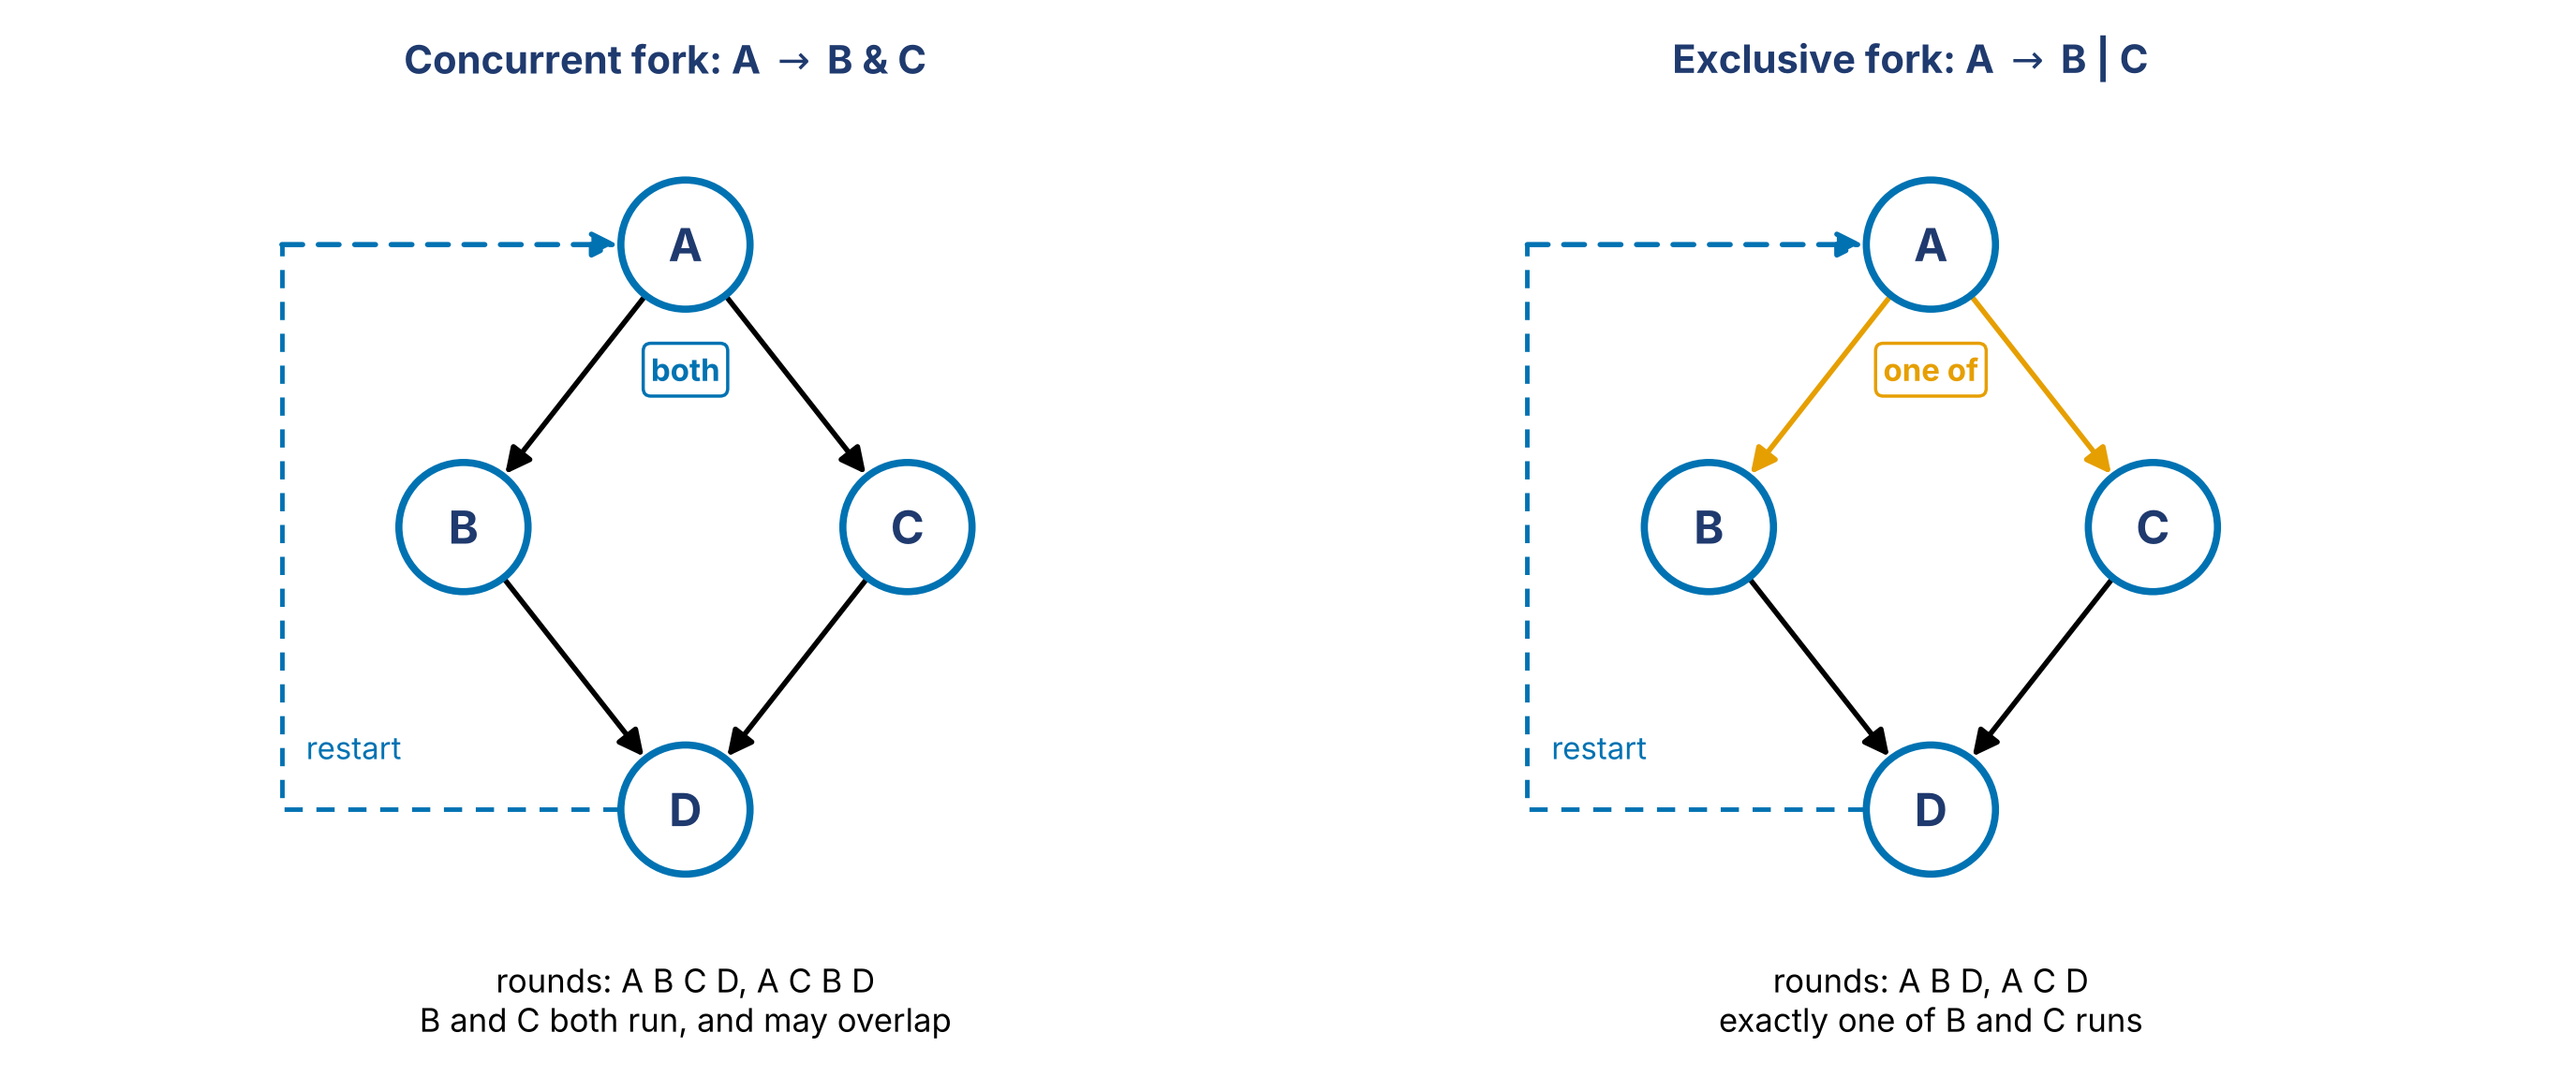
\includegraphics[width=0.85\textwidth]{contents/images/week-08/fork_two_meanings.png}
    \caption{Le stesse frecce, due significati. A sinistra fork \textbf{concorrente} (\texttt{A $\rightarrow$ B \& C}): B e C girano entrambi in ogni giro, anche sovrapposti, e D li aspetta tutti e due. A destra fork \textbf{esclusivo} (\texttt{A $\rightarrow$ B | C}): in ogni giro ne gira esattamente uno, e D aspetta solo quello.}
\end{figure}
Le frecce da sole non dicono quale dei due: \textbf{l'esercizio deve dirlo}. All'esame, se non è scritto, alza la mano e chiedi; se resta il dubbio, scrivi quale lettura hai usato. Un ordine si verifica \textbf{guardando gli archi}, uno per uno, non dividendo il grafo in ``livelli''.

\subsubsection*{3. Il metodo: un semaforo per arco}
È la base sicura, e la prima cosa da scrivere all'esame.
\begin{enumerate}
    \item Per ogni arco X $\rightarrow$ Y un semaforo \texttt{sXY} che parte da \textbf{0} (``in questo giro l'arco non è ancora stato attraversato'').
    \item Il semaforo del \textbf{restart} parte da \textbf{1}: quell'unico token fa partire il primo giro.
    \item Ogni task: \texttt{wait} una volta su ogni arco entrante, sezione critica, \texttt{signal} una volta su ogni arco uscente.
\end{enumerate}
Perché funziona (con fork concorrenti): ogni semaforo ha \textbf{un solo} task che fa signal e \textbf{un solo} task che fa wait, quindi un token non può finire al task sbagliato; un join passa i suoi wait in qualunque ordine e prosegue solo quando li ha tutti (il token arrivato prima resta nel semaforo); nessun task gira due volte in un giro, perché il suo token torna solo dopo il restart.

\subsubsection*{4. Togliere semafori: stessa fine sì, stesso inizio no}
Un token \textbf{non ha nome}: chi lo prende non sa chi l'ha dato.
\begin{itemize}
    \item \textbf{Condividere sul join è sicuro.} B $\rightarrow$ D e C $\rightarrow$ D usano un solo \texttt{sD} (counting, massimo 2): B e C danno un token ciascuno, D fa wait \textbf{due volte}. B non può dare un secondo token al posto di C, perché non può rigirare prima del restart.
    \item \textbf{Condividere sul fork concorrente è sbagliato.} A dà due token su un solo \texttt{sF}, B e C fanno wait una volta. Il conto torna, ma dopo la sua sezione critica B torna in cima al ciclo ed è \textbf{un altro task in attesa su \texttt{sF}}: può prendersi il token di C. Giro \textbf{A B B D}: C non gira mai, \textbf{nessun errore}, D conta due token ed è contento.
\end{itemize}
\begin{figure}[H]
    \centering
    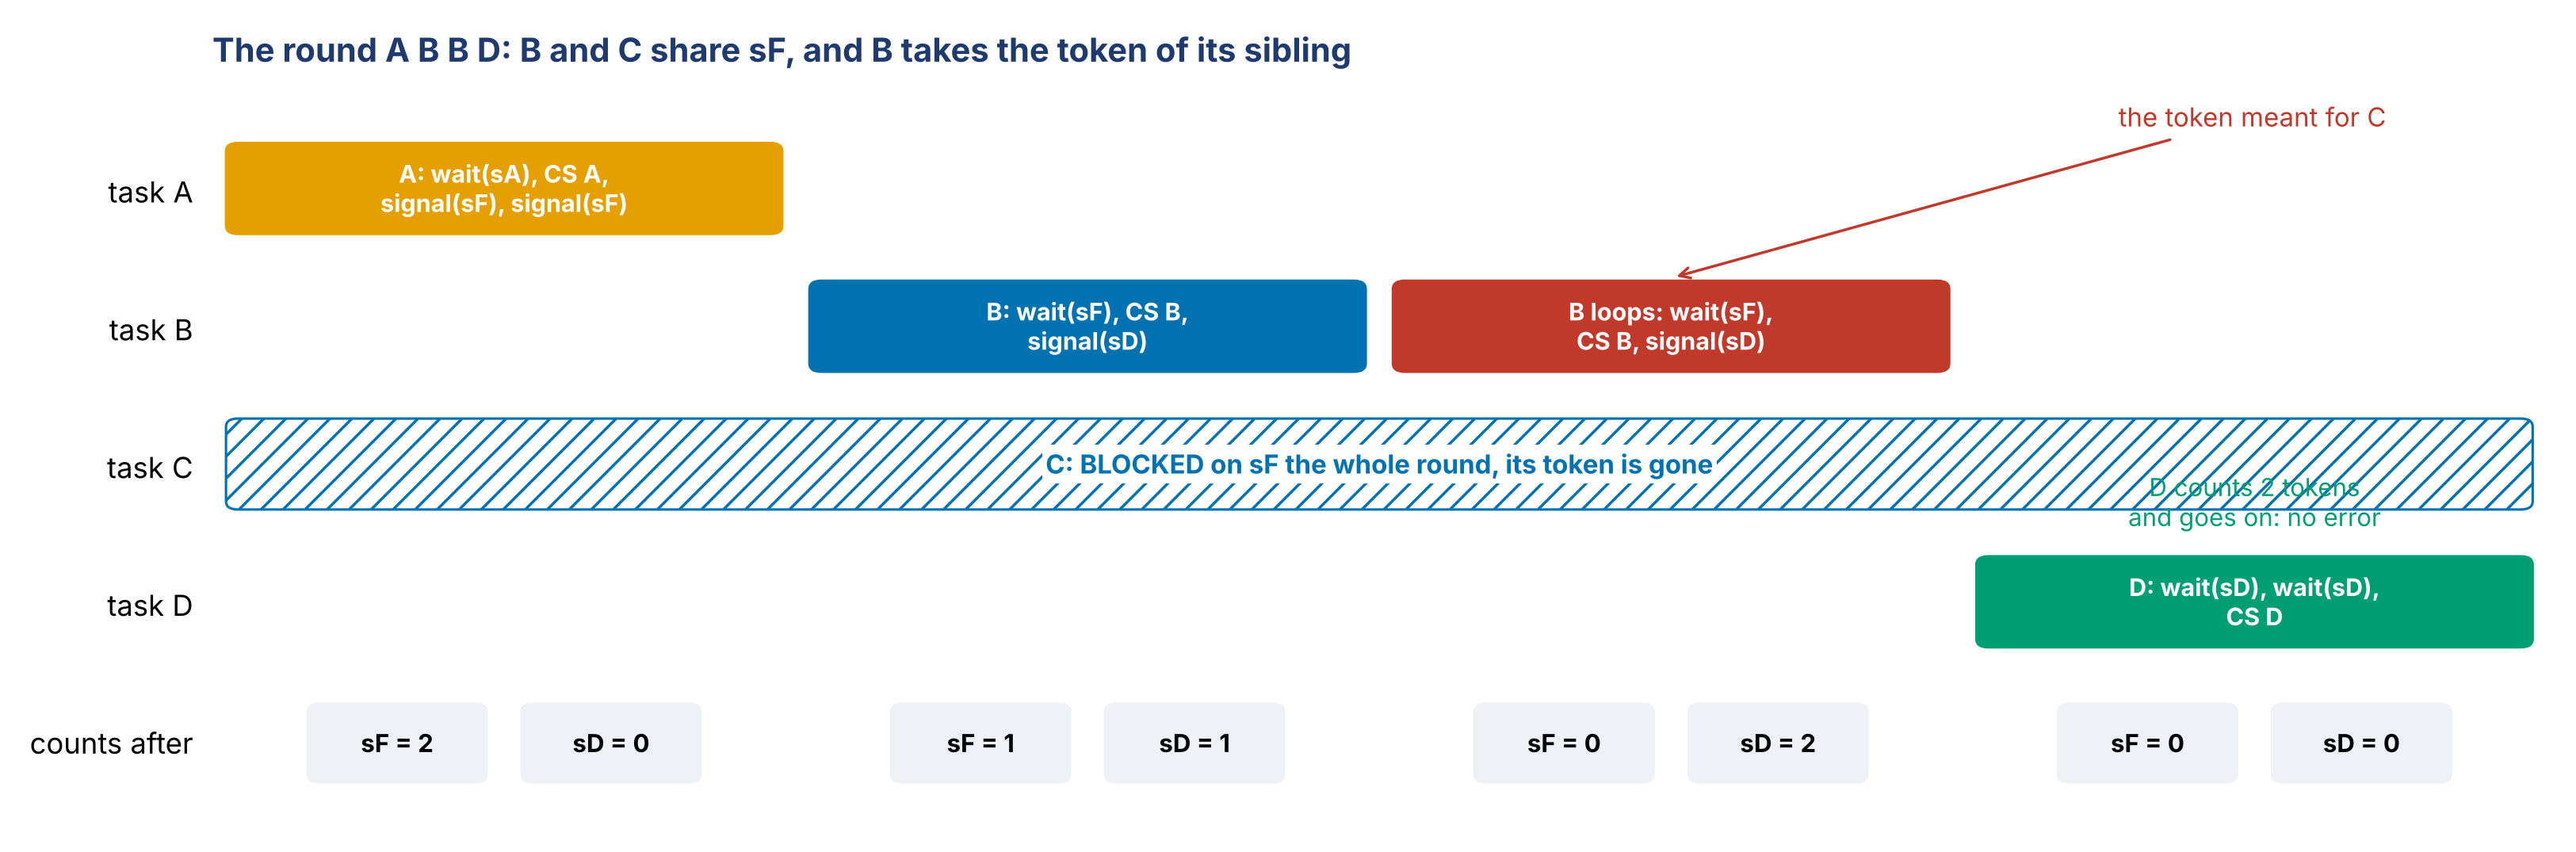
\includegraphics[width=0.9\textwidth]{contents/images/week-08/token_steal.png}
    \caption{Il furto del token: con \texttt{sF} condiviso, B gira due volte e C mai. È il ciclo infinito a rompere la condivisione: se ogni task girasse una volta sola, andrebbe bene.}
\end{figure}
\textbf{La regola}: due task che devono \emph{entrambi} girare in un giro non aspettano mai sullo stesso semaforo. Solo i rami di un fork \textbf{esclusivo} possono condividerne uno, segnalato \textbf{una volta}: un token, due pretendenti, ne entra uno. Da qui il \textbf{minimo}:
\begin{center}
\fbox{\parbox{0.85\textwidth}{\centering un semaforo per task, contando come uno i rami di un fork esclusivo}}
\end{center}
Ogni task aspetta sul suo semaforo una volta per arco entrante (una volta sola per un join di rami esclusivi). In FreeRTOS un semaforo che può ricevere più token è \textbf{counting}, con massimo uguale al numero di archi entranti; quello del restart è \texttt{xSemaphoreCreateCounting( 1, 1 )}; gli altri possono essere binari. Usare un counting dove bastava un binario non è penalizzato.

\subsubsection*{5. Concorrente contro esclusivo: dove cambia il codice}
\begin{center}
\small
\begin{tabular}{l P{0.27} P{0.27} P{0.17}}
    \hline
    & \textbf{chi fa il fork} & \textbf{i rami aspettano su} & \textbf{il join aspetta} \\
    \hline
    concorrente & signal su due semafori & il proprio semaforo & due volte \\
    esclusivo & signal su uno, una volta & lo stesso semaforo & una volta \\
    \hline
\end{tabular}
\end{center}
Nel fork esclusivo \textbf{chi vince non è deciso dai semafori}: nessuno promette che B e C si alternino, e uno dei due può non girare mai. Lo si vede in FreeRTOS nell'Unità 2.

\paragraph*{Gli errori tipici (Esempio 1).} Ogni riga è una sola modifica rispetto a una soluzione giusta:
\begin{center}
\small
\begin{tabular}{P{0.4} P{0.5}}
    \hline
    \textbf{errore} & \textbf{che cosa succede} \\
    \hline
    \texttt{sA} (il restart) parte da 0 & non gira niente: tutti aspettano un token che nessuno può dare \\
    concorrente: D fa wait su \texttt{sD} una volta sola & D parte dopo il primo dei due: giro A B D con C ancora da fare \\
    \texttt{sD} binario, B e C danno prima che D prenda & il secondo give trova il semaforo pieno, il token si perde, D aspetta per sempre (bug raro e nascosto) \\
    esclusivo: A fa signal su \texttt{sF} due volte & girano entrambi i rami, e a D avanza un token per il giro dopo \\
    esclusivo: D fa wait due volte & il secondo token non arriva mai: il primo giro non finisce \\
    \hline
\end{tabular}
\end{center}
Anche i test possono non vedere questi errori (se le priorità fanno girare C presto, l'ordine sbagliato non compare): si ragiona su \textbf{tutte} le esecuzioni possibili. All'esame la soluzione col metodo è accettata, quella ottima prende più punti, quella sbagliata zero: se non sei sicuro, il metodo meccanico è il livello minimo garantito.

\subsubsection*{6. Il buffer limitato (produttore e consumatore)}
Tre bisogni diversi, tre semafori: \texttt{empty} $=$ N (posti liberi), \texttt{full} $=$ 0 (posti pieni), \texttt{mutex} $=$ 1 (un task alla volta sul buffer e sull'indice). Il produttore fa \texttt{wait( empty ); wait( mutex );} scrive in \texttt{buffer[ in ]}, incrementa \texttt{in} modulo N, \texttt{signal( mutex ); signal( full );}. Il consumatore è lo specchio, con \texttt{full} ed \texttt{empty} scambiati e \texttt{out} al posto di \texttt{in}.
\begin{itemize}
    \item \textbf{Perché due contatori?} Ai due estremi l'ordine è obbligato: buffer vuoto, solo il produttore può andare; buffer pieno, solo il consumatore. Un solo contatore non può fermare uno su ``nessun posto libero'' e l'altro su ``nessun posto pieno''.
    \item \textbf{Scambiare i due wait} del produttore: a buffer pieno tiene \texttt{mutex} e dorme su \texttt{empty}, il consumatore si blocca su \texttt{mutex}: \textbf{deadlock}. L'ordine dei wait conta.
    \item \textbf{Scambiare i due signal}: niente di grave, un signal non blocca mai.
    \item Con \textbf{un} produttore e \textbf{un} consumatore \texttt{mutex} si può togliere (\texttt{in} e \texttt{out} hanno un solo padrone ciascuno); con \textbf{due} produttori no: condividono \texttt{in}, ed è il lost update della settimana 7.
    \item Con N $=$ 1 produttore e consumatore si alternano: metti, prendi, metti, \dots
\end{itemize}

\subsubsection*{7. Lettori e scrittori}
I lettori possono stare dentro \textbf{insieme}, uno scrittore deve stare \textbf{da solo}. Un mutex semplice è corretto ma troppo severo. L'idea è una stanza con un lucchetto, \texttt{rw}: lo scrittore lo chiude per sé; i lettori lo chiudono \textbf{come gruppo}, il \textbf{primo} che entra lo chiude e l'\textbf{ultimo} che esce lo riapre. Per sapere chi è primo e ultimo tengono un contatore \texttt{readers}, protetto da \texttt{mutex}.
\begin{itemize}
    \item \textbf{Perché \texttt{mutex}?} Incremento e test devono essere un passo solo: senza, R1 e R2 incrementano entrambi prima di testare, nessuno dei due vede \texttt{readers == 1}, nessuno chiude \texttt{rw}, e lo scrittore entra mentre loro leggono.
    \item \texttt{mutex} è tenuto solo per aggiornare il contatore: durante la lettura è libero.
    \item \textbf{\texttt{rw} non può essere un mutex di FreeRTOS}: il mutex ha un proprietario, e qui lo prende il primo lettore e lo rilascia l'ultimo, che può essere un altro task. Si usa \texttt{xSemaphoreCreateCounting( 1, 1 )}.
    \item \textbf{Starvation dello scrittore}: se i lettori continuano ad arrivare sovrapposti, \texttt{rw} non viene mai rilasciato. La soluzione è ingiusta per gli scrittori; le versioni più giuste usano più semafori.
\end{itemize}
Buffer limitato e lettori/scrittori non sono solo esercizi: sono \textbf{design pattern} che tornano nella seconda parte dell'esame, quando bisogna scrivere un'applicazione FreeRTOS.

\subsection{Unità 2}
\paragraph*{L'idea.} Su carta abbiamo usato solo semafori. FreeRTOS offre oggetti diversi per problemi diversi: si parte dal \textbf{requisito} e si sceglie l'oggetto. I programmi sono in \texttt{freertos-labs/week-08/}: \texttt{base/} da completare (ogni punto ha un commento marker), \texttt{solution/} commentata riga per riga; il kernel non si tocca mai. \texttt{make APP=<programma> DEMO=<variante> run}, e si esce con \texttt{Ctrl-C}.

\subsubsection*{1. Quattro meccanismi}
\begin{center}
\small
\begin{tabular}{P{0.18} P{0.1} P{0.36} P{0.22}}
    \hline
    \textbf{oggetto} & \textbf{parte} & \textbf{a che serve} & \textbf{programma} \\
    \hline
    semaforo binario & vuoto & ``è successo'': un task avvisa un altro (Y dopo X) & \texttt{precedence} \\
    semaforo counting & qualsiasi & contare eventi o risorse (un join) & \texttt{precedence} \\
    mutex & libero & un task alla volta su dati condivisi; ha un \textbf{proprietario} & \texttt{deadlock} \\
    coda & vuota & passare \textbf{dati} tra task (produttore/consumatore, gatekeeper) & \texttt{prodcons}, \texttt{gatekeeper} \\
    \hline
\end{tabular}
\end{center}
\begin{itemize}
    \item I tre semafori hanno lo stesso tipo \texttt{SemaphoreHandle\_t} (header \texttt{semphr.h}) e le stesse due chiamate, \texttt{xSemaphoreTake} e \texttt{xSemaphoreGive}. La coda ha \texttt{QueueHandle\_t}, \texttt{xQueueSend} e \texttt{xQueueReceive}.
    \item \textbf{Binario e mutex sono diversi dal primo take}: il binario parte vuoto, il take blocca (serve a \textbf{segnalare}); il mutex parte libero, il take riesce e il chiamante ne diventa \textbf{proprietario} (serve a \textbf{proteggere}). Un give su un mutex tenuto da un altro task, con \texttt{configASSERT} attivo, ferma il programma con un'asserzione.
    \item \texttt{xQueueCreate( lunghezza, sizeof( item ) )}: servono entrambi per allocare la memoria. Gli elementi sono \textbf{copiati}: dopo il send si può riusare la variabile. Mai mandare un puntatore a una variabile locale: si copierebbe il puntatore, non i dati.
    \item \texttt{uxSemaphoreGetCount} e \texttt{uxQueueSpacesAvailable} servono \textbf{solo a guardare} (per stampare), non a decidere: il valore può cambiare subito dopo.
\end{itemize}

\subsubsection*{2. Il task event-driven}
Il task periodico della settimana 7 si sveglia su un orologio; il task \textbf{event-driven} (aperiodico) si sveglia quando succede qualcosa:
\begin{lstlisting}[language=C, showstringspaces=false, basicstyle=\ttfamily\footnotesize]
for( ;; )
{
    xSemaphoreTake( xEvent, portMAX_DELAY );   /* BLOCKED fino all'evento */
    /* gestisce l'evento */
}
\end{lstlisting}
Mentre aspetta non usa CPU (gira l'idle). Il ciclo di vita ha tre transizioni: BLOCKED $\rightarrow$ READY (qualcuno fa give), READY $\rightarrow$ RUNNING (lo sceglie lo scheduler: se è il più prioritario, subito), RUNNING $\rightarrow$ BLOCKED (ha finito e richiama il take). Con \texttt{xQueueReceive} al posto del take, l'evento porta anche dei dati.

\subsubsection*{3. Timeout e codici di ritorno}
\begin{center}
\small
\begin{tabular}{P{0.3} P{0.6}}
    \hline
    \textbf{timeout} & \textbf{se l'oggetto non è pronto} \\
    \hline
    \texttt{0} & ritorna subito con un codice di errore \\
    \texttt{pdMS\_TO\_TICKS( 300 )} & BLOCKED al massimo 300\,ms, poi codice di errore \\
    \texttt{portMAX\_DELAY} & BLOCKED finché serve (richiede \texttt{INCLUDE\_vTaskSuspend} $=$ 1) \\
    \hline
\end{tabular}
\end{center}
Successo: \texttt{pdTRUE} (semafori) o \texttt{pdPASS} (code, stesso valore). Fallimento: \texttt{pdFALSE}, \texttt{errQUEUE\_FULL}, \texttt{errQUEUE\_EMPTY} (tutti 0). Un give fallisce solo su semaforo pieno: non aspetta mai. \textbf{Regola}: con un timeout finito controlla sempre il valore di ritorno, e dopo un fallimento \textbf{non hai niente in mano}: non fare il give di ciò che non hai preso. Con \texttt{portMAX\_DELAY} la chiamata torna solo a successo, quindi non serve testarla. All'esame il sito di FreeRTOS con la documentazione è accessibile: serve sapere \emph{cosa} cercare, non gli argomenti a memoria.

\subsubsection*{4. \texttt{precedence}: il grafo vince sulle priorità}
L'Esempio 1 concorrente con quattro semafori. Le priorità sono messe apposta al contrario: A 1 (la più bassa), B 2, C 3, D 4. Senza semafori D girerebbe per primo.
\begin{itemize}
    \item \textbf{Dove si dichiarano?} Fuori da ogni funzione, \texttt{static}. Globali, perché ogni task ha il suo stack e i task non si vedono gli stack a vicenda; \texttt{static}, perché sono visibili solo in questo file e non vanno in conflitto con nomi uguali di altre librerie.
    \item \textbf{Dove si creano?} In \texttt{main}, prima di \texttt{vTaskStartScheduler}, \textbf{una volta sola}: creandoli dentro i task se ne farebbero due copie diverse, e il secondo \emph{create} cancellerebbe lo stato del primo.
    \item \textbf{Una funzione di task non deve mai ritornare}: con il \texttt{for( ;; )} non succede; se un task deve finire, va sospeso (\texttt{vTaskSuspend( NULL )}).
    \item L'ordine dei due give di A non conta: l'obiettivo è abilitare entrambi.
    \item \textbf{Il risultato}: ogni giro è A B C D, cominciando dalla priorità più bassa. I semafori decidono cosa è \textbf{permesso}, qualunque cosa dicano le priorità.
\end{itemize}
\begin{figure}[H]
    \centering
    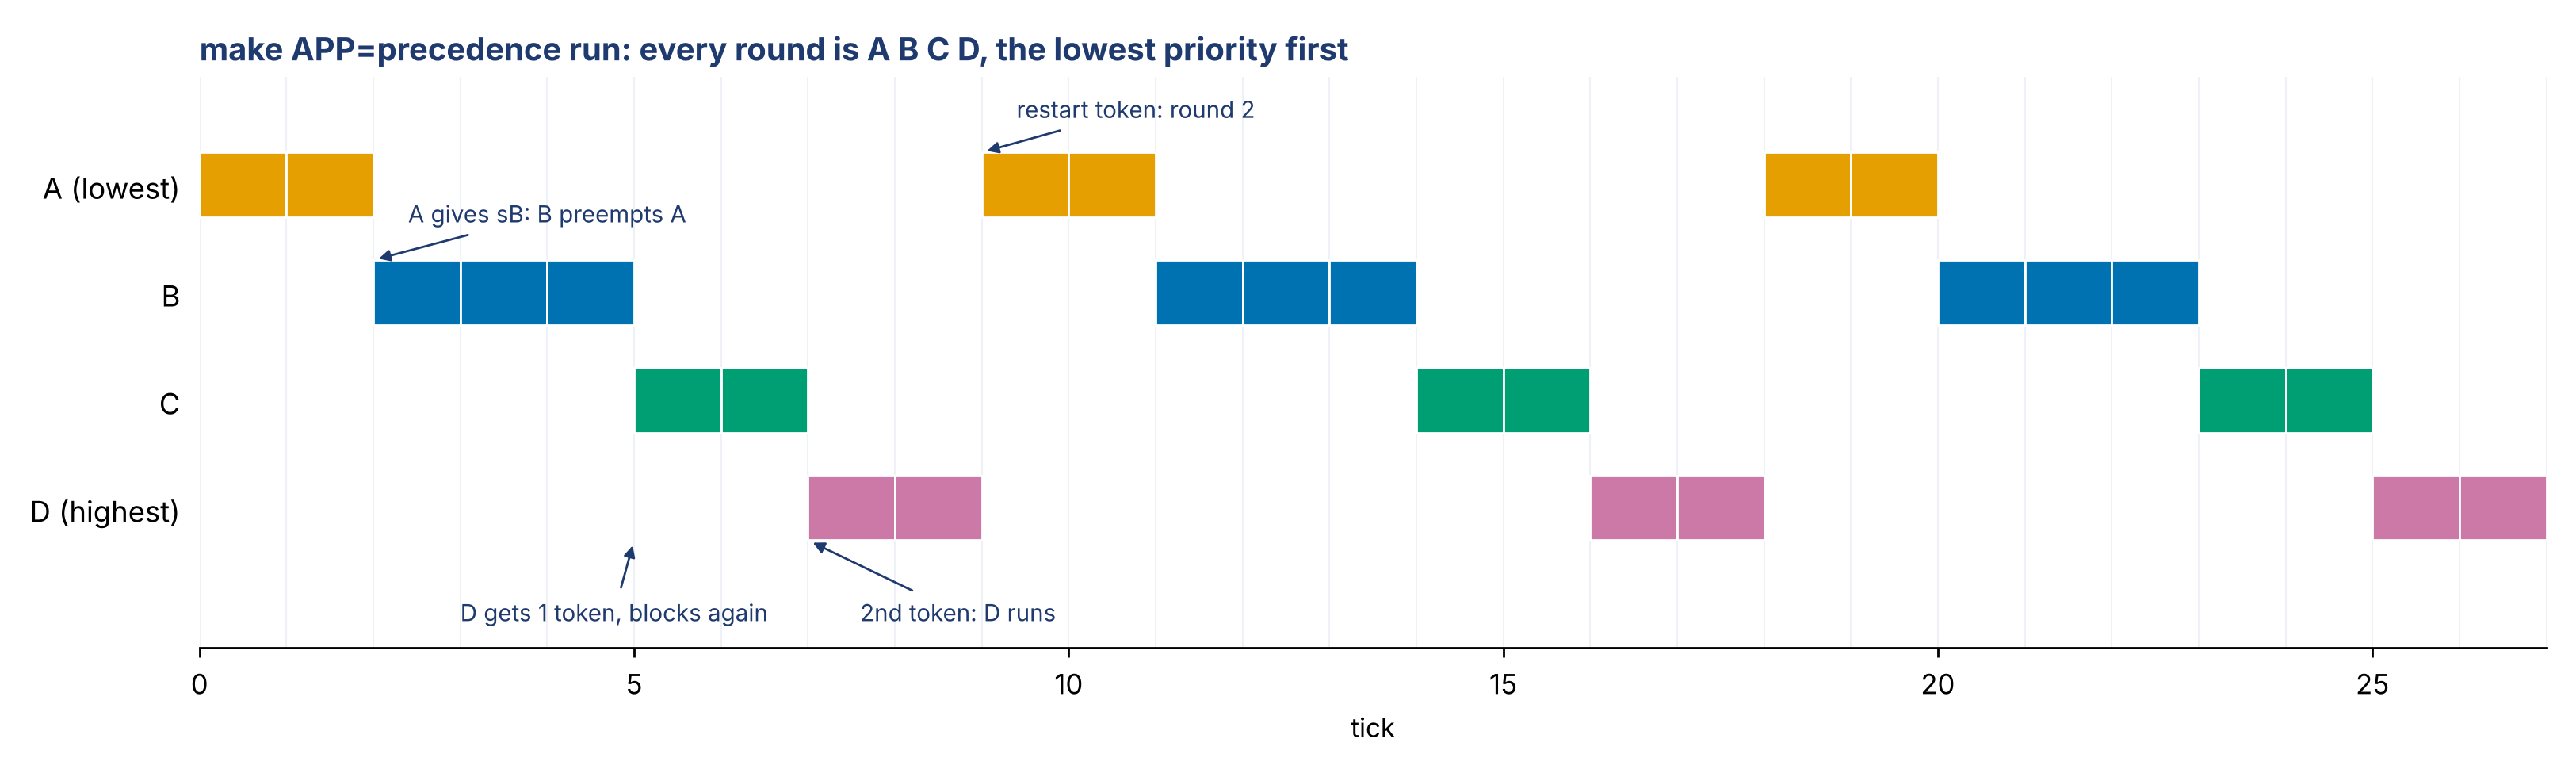
\includegraphics[width=0.95\textwidth]{contents/images/week-08/precedence_trace.png}
    \caption{La traccia di \texttt{precedence}: CPU \texttt{AABBBCCDD} ripetuto. Notare che B prelaziona A \emph{dentro} \texttt{xSemaphoreGive( sB )}: A darà \texttt{sC} solo quando B si blocca di nuovo.}
\end{figure}
Per leggere la traccia: una riga \texttt{T <tick> <da> <a>} è un cambio di task. Al tick 0 R, D, C e B si bloccano subito sui loro semafori (tutti allo stesso tick, perché non usano CPU), e solo A può andare avanti. Quando un task più prioritario viene svegliato da un give, prelaziona chi ha fatto il give \textbf{all'interno} della chiamata.

\subsubsection*{5. \texttt{DEMO=steal} e \texttt{DEMO=xor}: le priorità scelgono}
\begin{itemize}
    \item \textbf{\texttt{steal}} (\texttt{sB} e \texttt{sC} sono lo stesso semaforo, e A dà due token): C gira due volte per giro e B mai. Al primo token si sveglia il task in attesa più prioritario, C; C torna in cima al ciclo e, essendo ancora il più prioritario, prende anche il secondo. Con altre priorità il ladro sarebbe B: \textbf{il bug è nei semafori, le priorità scelgono solo il ladro}.
    \item \textbf{\texttt{xor}} (fork esclusivo, un token): i giri sono tutti validi (A C D), ma B \textbf{non gira mai}, è in \textbf{starvation}. Con B e C alla \textbf{stessa} priorità si alternano (A B D, A C D, \dots), perché a parità di priorità vale l'ordine di arrivo.
\end{itemize}
\textbf{I semafori fissano ciò che è permesso, le priorità scelgono tra gli ordini permessi.}

\subsubsection*{6. Dentro il kernel, in breve}
\begin{itemize}
    \item \textbf{Un semaforo è una coda} con elementi di dimensione 0, e il suo contatore è il numero di elementi (\texttt{uxMessagesWaiting}). Semafori, mutex e code bloccano e svegliano con \textbf{lo stesso codice}; il mutex aggiunge solo il proprietario.
    \item Ogni oggetto ha \textbf{due liste d'attesa}, \textbf{ordinate per priorità}: si sveglia la testa, e a parità di priorità chi è arrivato prima. Sono:
    \newline\texttt{xTasksWaitingToSend} e \texttt{xTasksWaitingToReceive}; per un semaforo si usa solo la seconda.
    \item Un task in attesa sta su \textbf{due} liste: quella dell'oggetto (``è arrivato l'evento'') e quella dei delayed (``è scaduto il timeout''); con \texttt{portMAX\_DELAY}, quella dei sospesi.
    \item \textbf{Un task risvegliato ritesta}: un altro può aver preso il token prima di lui.
    \item \textbf{Il trace} (opzionale): FreeRTOS chiama la macro \texttt{traceTASK\_SWITCHED\_IN} a ogni cambio di task; la nostra configurazione la definisce. Siccome gira dentro il context switch, \textbf{non stampa}: copia tre valori in un ring buffer, e la stampa la fa dopo un task normale. Regola generale: dentro un context switch fai il meno possibile.
\end{itemize}

\subsubsection*{7. \texttt{prodcons}: la coda fa tutto}
Produttore veloce (1 tick), consumatore lento (5 tick), coda di 4 elementi, 12 numeri.
\begin{figure}[H]
    \centering
    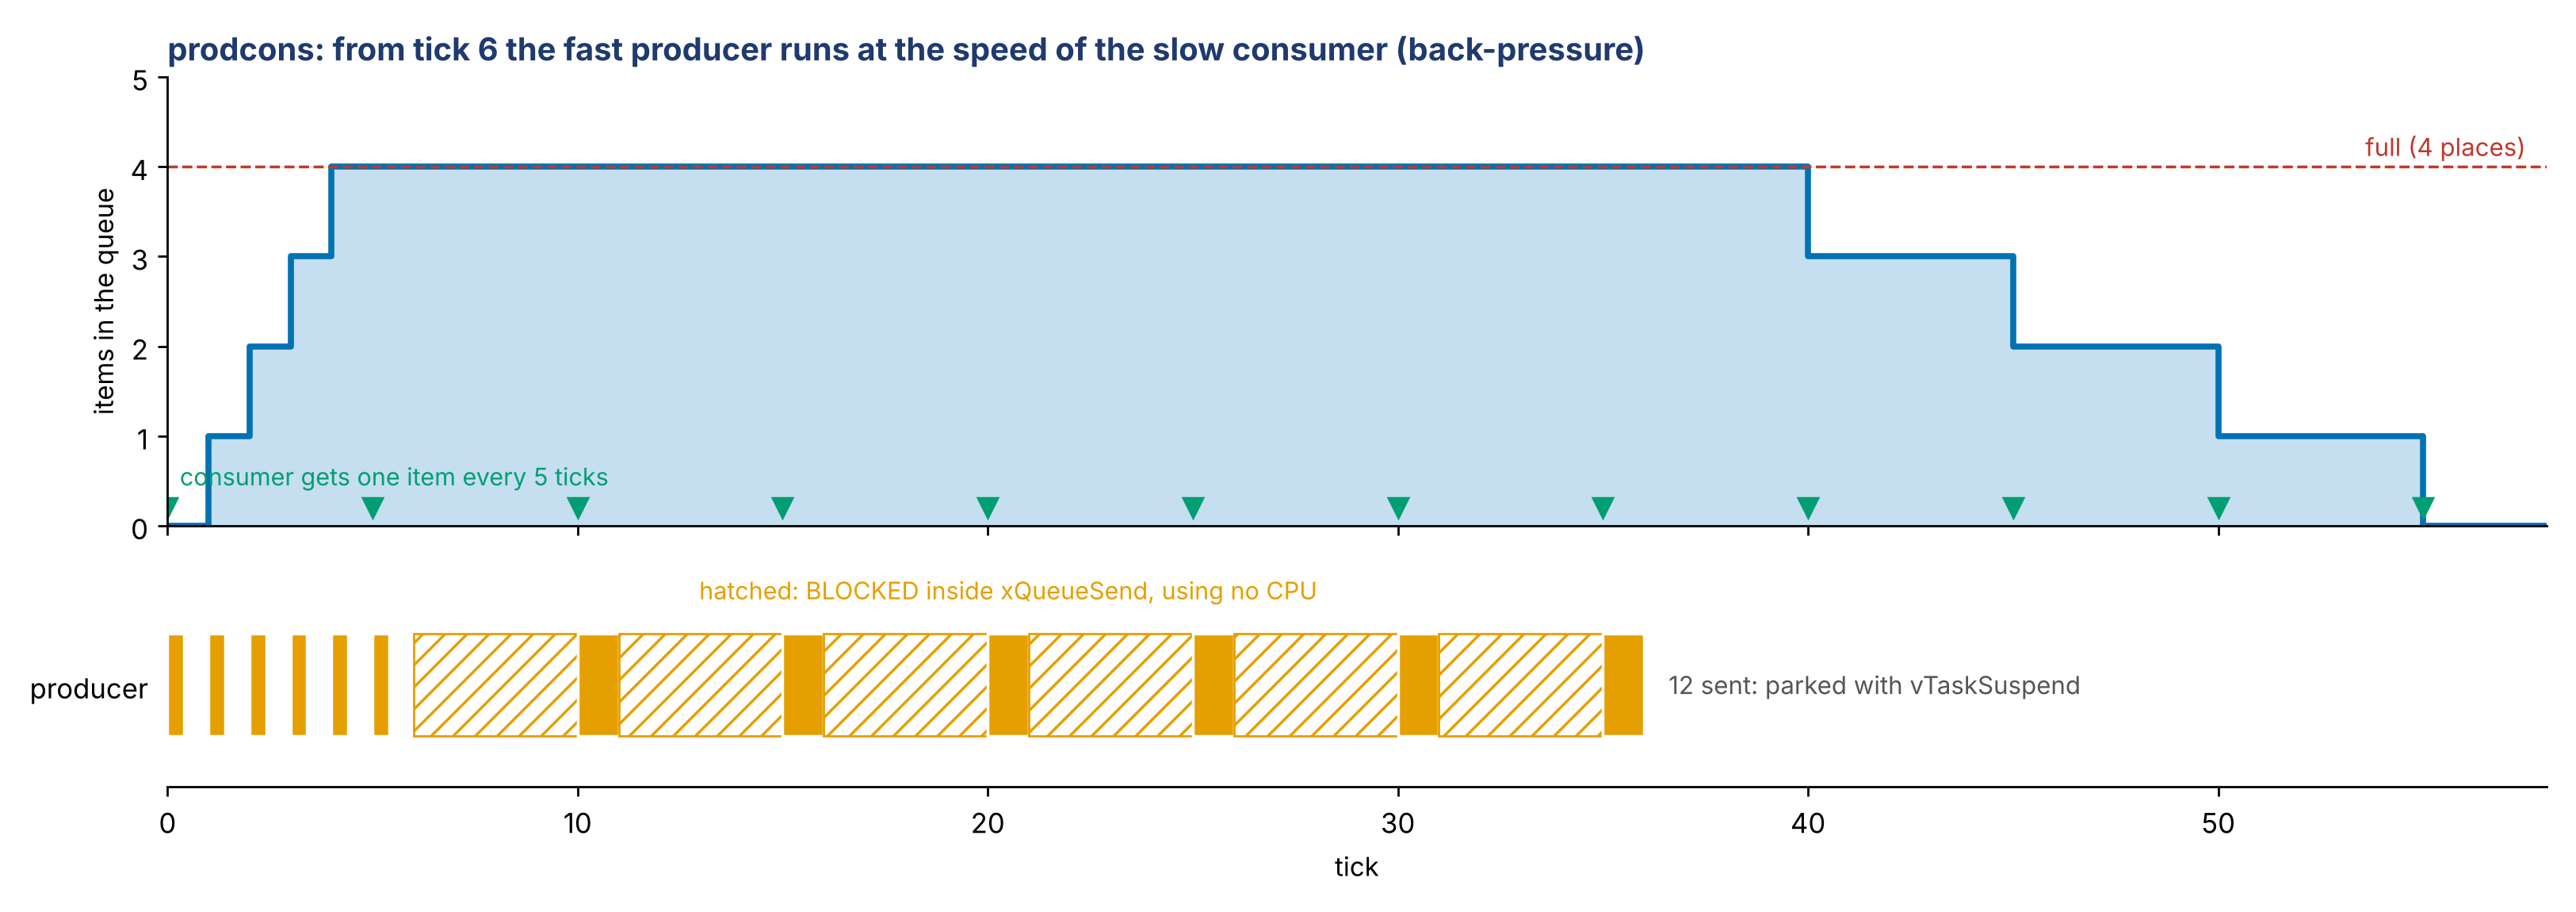
\includegraphics[width=0.95\textwidth]{contents/images/week-08/prodcons_fill.png}
    \caption{I primi numeri riempiono la coda; dal tick 6 il produttore è BLOCKED dentro \texttt{xQueueSend} e da lì va alla velocità del consumatore: \textbf{back-pressure}.}
\end{figure}
Nessun ciclo che controlla il buffer, nessun lock nel codice. \texttt{DEMO=sem} rifà lo stesso buffer a mano con \texttt{empty}, \texttt{full} e \texttt{mutex} e stampa \textbf{esattamente le stesse righe, tick per tick}: la coda contiene i due contatori con le loro liste d'attesa, una breve sezione critica al posto del mutex, e la memoria con le posizioni di lettura e scrittura.

\subsubsection*{8. Il gatekeeper: un proprietario invece della condivisione}
Contro l'output mescolato si può mettere un lock sulla UART, oppure darle \textbf{un solo proprietario}. Il \textbf{gatekeeper} è l'unico task che tocca la UART; S1 e S2 costruiscono una riga intera in una variabile locale (\texttt{line\_t}, 64 byte) e ne mandano una \textbf{copia} alla coda. Nessuna riga si mescola (748 su 748 intere in 32\,s), e nessun lock.
\begin{itemize}
    \item \textbf{La lunghezza della coda è la riga più delicata}: con lunghezza 1 la stampa diventa una mutua esclusione (chi arriva dopo aspetta il gatekeeper); più è lunga, più spesso un task trova posto e prosegue subito, perché copiare in memoria è velocissimo mentre la UART è lentissima.
    \item \textbf{Priorità del gatekeeper}: nel programma è 2, sopra i mittenti (1), quindi stampa appena arriva una riga. Per il professore può anche essere bassa, come l'idle: le righe restano intere, e se i mittenti vanno più veloci la coda si riempie e si bloccano (back-pressure, non mescolamento).
    \item È la stessa idea del \textbf{tracing} e del logging nei sistemi embedded: si registra in memoria, un task a bassa priorità stampa o salva su flash.
\end{itemize}
\begin{center}
\footnotesize
\begin{tabular}{P{0.16} P{0.24} P{0.24} P{0.24}}
    \hline
    & \textbf{spinlock} & \textbf{sezione critica} & \textbf{gatekeeper} \\
    \hline
    chi aspetta & l'altro task, girando sulla CPU & nessuno: niente switch finché la riga non è uscita & un mittente, BLOCKED, solo a coda piena \\
    interrupt mascherati? & no & sì (BASEPRI), anche il tick & no (solo la breve copia del kernel) \\
    costo & CPU sprecata & sistema fermo per tutta la riga & un task in più, una coda, le copie \\
    \hline
\end{tabular}
\end{center}

\subsection{Unità 3}
\paragraph*{L'idea.} Due task che prendono due risorse in \textbf{ordine opposto} possono bloccarsi a vicenda per sempre, senza nessun errore. Bisogna saper riconoscere quando può succedere (quattro condizioni, un grafo), sapere come impedirlo, e saperlo scovare in un programma vero.

\subsubsection*{1. Deadlock e starvation}
\begin{lstlisting}[basicstyle=\ttfamily\footnotesize]
semaphore S = 1, Q = 1;
T1:  wait( S );  print A;  wait( Q );  ...
T2:  wait( Q );  print C;  wait( S );  ...
\end{lstlisting}
Se entrambi superano il primo wait, T1 tiene \texttt{S} e aspetta \texttt{Q}, T2 tiene \texttt{Q} e aspetta \texttt{S}: nessuno dei due arriverà mai al signal. È questione di sfortuna, solo alcuni interleaving ci arrivano.
\begin{itemize}
    \item \textbf{Deadlock}: un insieme di task in cui ognuno aspetta qualcosa che solo un altro task dell'insieme può dare. Nessuno di loro girerà mai più. Si corregge cambiando la \textbf{sincronizzazione dell'applicazione}.
    \item \textbf{Starvation}: il task \emph{potrebbe} girare, ma altri passano sempre prima. È un problema di prestazioni del \textbf{sistema operativo} (dello scheduler).
    \item Nessun fault, nessun errore: i task sono semplicemente BLOCKED e il resto del sistema continua.
\end{itemize}

\subsubsection*{2. Le quattro condizioni necessarie (Coffman)}
Il deadlock è possibile solo se valgono \textbf{tutte e quattro} insieme. Togline una e non può succedere.
\begin{center}
\small
\begin{tabular}{P{0.18} P{0.32} P{0.4}}
    \hline
    \textbf{condizione} & \textbf{nell'esempio} & \textbf{come romperla (prevenzione)} \\
    \hline
    mutua esclusione & un semaforo a 1 fa entrare un task & risorsa condivisibile, o un proprietario (gatekeeper) \\
    hold and wait & T1 tiene \texttt{S} e aspetta \texttt{Q} & prendere tutto insieme, o non tenere niente mentre si aspetta \\
    no preemption & solo chi tiene il token lo rilascia & se il secondo take fallisce, rilasciare il primo e riprovare (il lavoro fatto si butta) \\
    attesa circolare & T1 aspetta T2, T2 aspetta T1 & \textbf{lock ordering}: tutti prendono le risorse nello stesso ordine \\
    \hline
\end{tabular}
\end{center}

\subsubsection*{3. Il grafo di allocazione delle risorse}
Cerchi i task, quadrati le risorse; arco \textbf{richiesta} task $\rightarrow$ risorsa (aspetta), arco \textbf{assegnazione} risorsa $\rightarrow$ task (la tiene).
\begin{figure}[H]
    \centering
    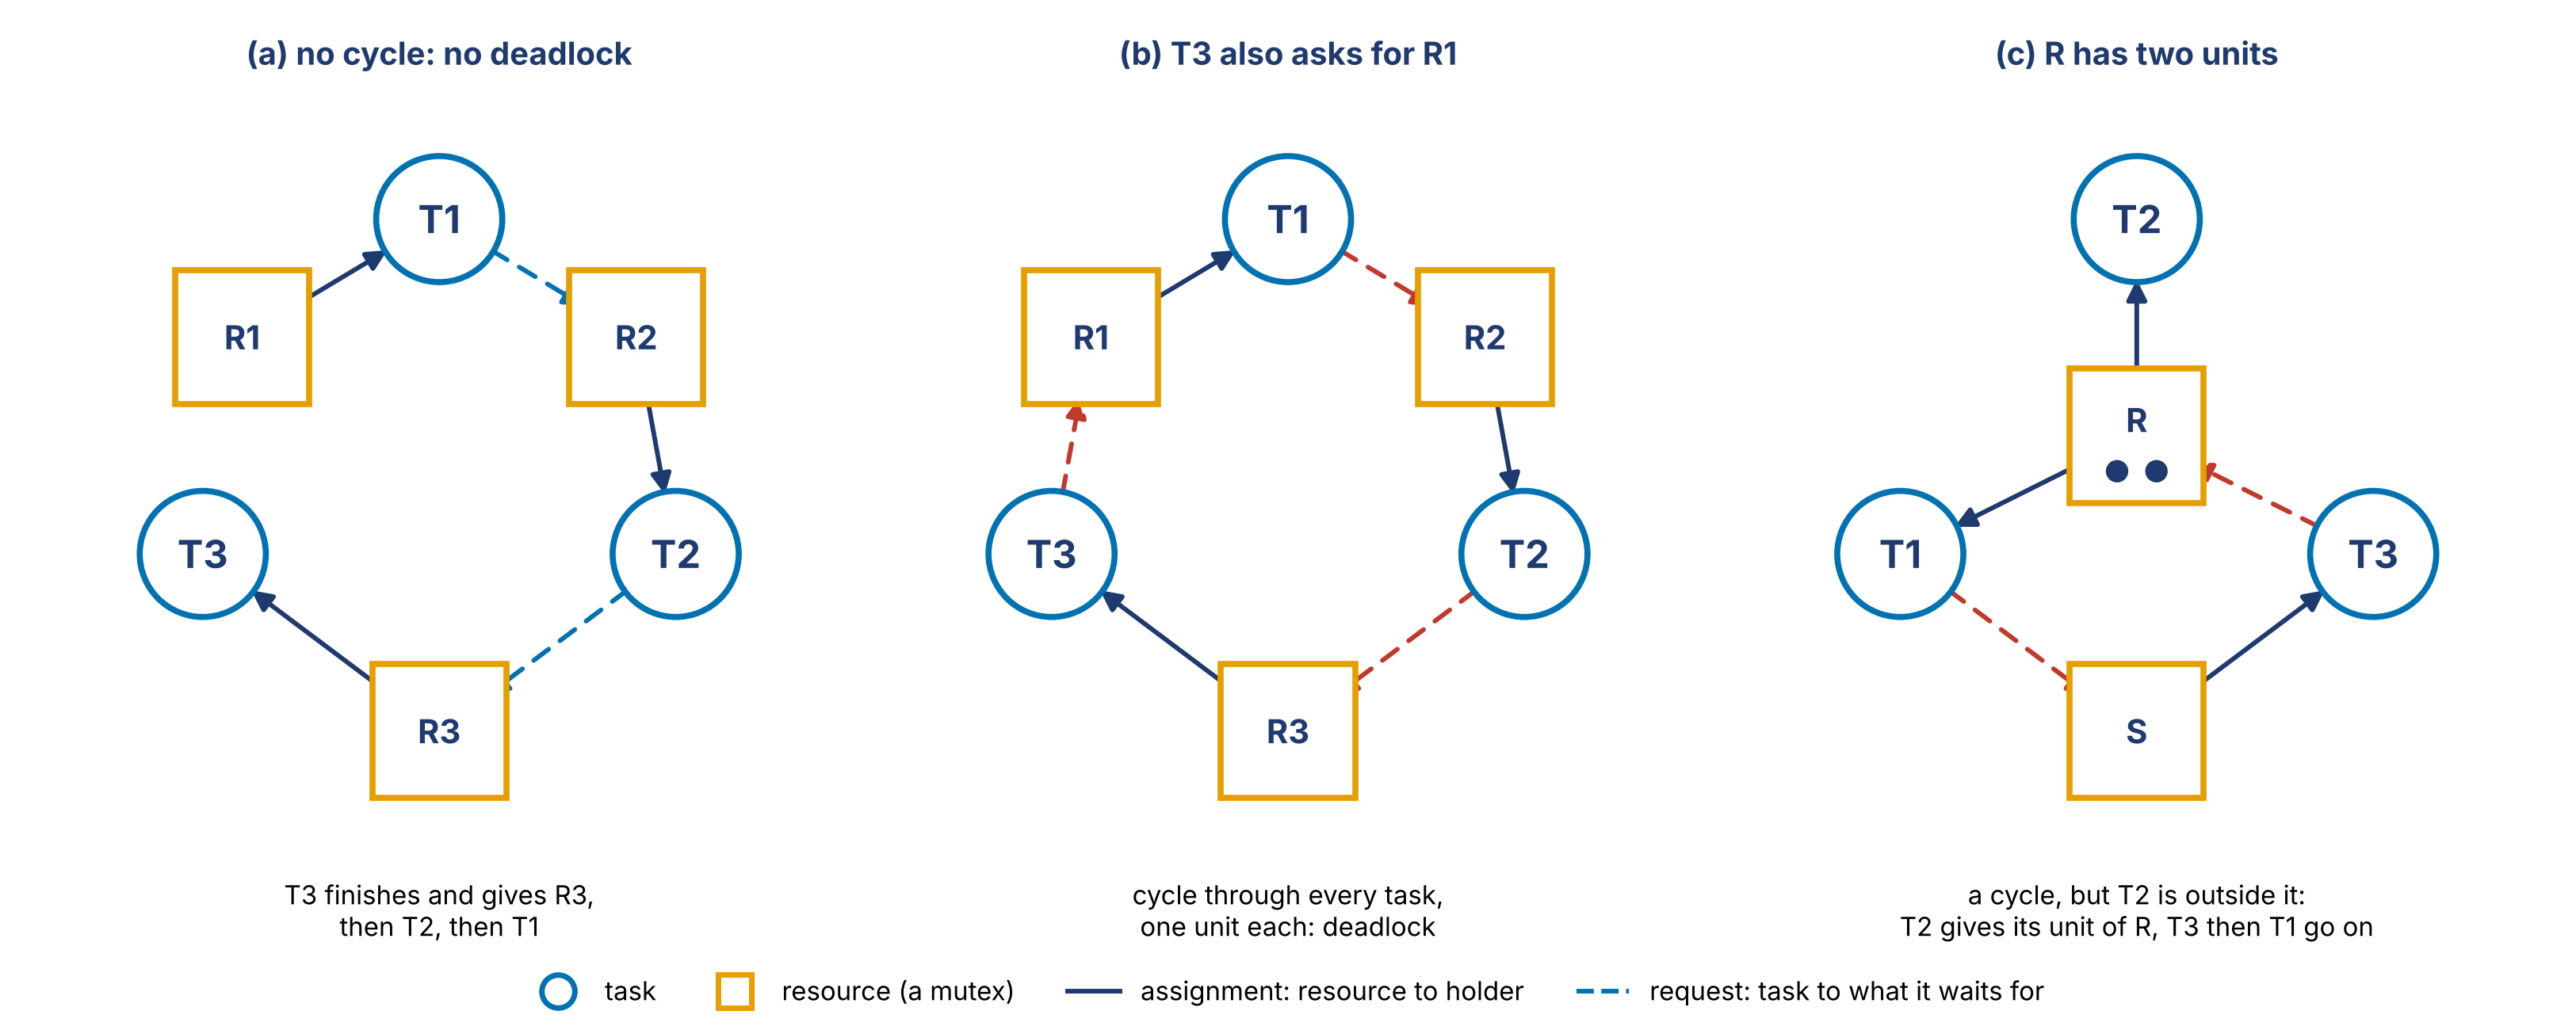
\includegraphics[width=1\textwidth]{contents/images/week-08/rag_examples.png}
    \caption{(a) Nessun ciclo, nessun deadlock: T3 finisce, poi T2, poi T1. (b) Ciclo con risorse a una unità: deadlock. (c) Ciclo, ma R ha due unità e T2, fuori dal ciclo, può finire e liberarne una: nessun deadlock.}
\end{figure}
\textbf{Regola}: con risorse a una unità (come i mutex) ciclo $\Leftrightarrow$ deadlock. Con più unità il ciclo è \textbf{necessario ma non sufficiente}: bisogna ragionare su cosa può finire.

\subsubsection*{4. Tre strategie, e il lock ordering}
\begin{itemize}
    \item \textbf{Prevenzione}: quando scrivi il codice, rendi impossibile una condizione. Costo a run time nullo: è la scelta dei sistemi embedded (un prodotto non può aspettare che qualcuno lo riavvii).
    \item \textbf{Avoidance}: a ogni richiesta il kernel concede la risorsa solo se resta uno stato \textbf{sicuro} (esiste un ordine in cui tutti finiscono). Algoritmo del banchiere; poco usata nei sistemi piccoli (massimi difficili da conoscere, controllo a ogni richiesta).
    \item \textbf{Rilevamento e recupero}: si lascia accadere e poi si rompe il ciclo (uccidere un task, togliere una risorsa). In pratica: un task \textbf{monitor} che controlla che gli altri facciano progressi.
\end{itemize}
Il costo a run time cresce nell'ordine. \textbf{Lock ordering}: numera i mutex, ogni task li prende in ordine \textbf{crescente}. Un ciclo richiederebbe $a < b < \dots < z < a$, impossibile. Se un task tiene M2 e scopre di aver bisogno di M1, deve rilasciare M2, prendere M1, riprendere M2 e \textbf{ricontrollare} i dati, perché nel frattempo possono essere cambiati.

\subsubsection*{5. I filosofi a cena}
Cinque filosofi, cinque forchette (mutex), ognuno ne vuole due: sinistra e poi destra. Se prendono tutti la sinistra insieme, deadlock (tutte e quattro le condizioni); bastano quattro filosofi al tavolo per non averlo.
\begin{center}
\small
\begin{tabular}{P{0.5} P{0.4}}
    \hline
    \textbf{correzione} & \textbf{condizione rotta} \\
    \hline
    forchette numerate, prima quella col numero più basso (P5 prende F1 e poi F5) & attesa circolare (lock ordering) \\
    un semaforo counting a 4: solo quattro al tavolo & attesa circolare \\
    prendere le due forchette solo se sono libere entrambe, in un passo atomico & hold and wait \\
    \hline
\end{tabular}
\end{center}

\subsubsection*{6. Message passing}
Invece di condividere una variabile, i task si mandano \textbf{messaggi} (\texttt{send}, \texttt{receive}). Tre domande di progetto:
\begin{itemize}
    \item \textbf{Naming}: \textbf{diretto} (\texttt{send( T2, m )}: serve un instradamento nel sistema, costa CPU) o \textbf{indiretto} (\texttt{send( Q, m )} su una \textbf{mailbox}: costa una connessione per ogni coppia che parla).
    \item \textbf{Sincronizzazione}: \textbf{sincrona} (bloccante: non si spreca CPU, ma non sai quando ti svegli) o \textbf{asincrona} (torna subito: rischi di finire in polling). Se send e receive si aspettano a vicenda: \textbf{rendezvous}. Niente è perfetto, è sempre un compromesso.
    \item \textbf{Buffering}: \textbf{zero} posti (sempre rendezvous), \textbf{limitato} a N (il mittente aspetta solo a coda piena), \textbf{illimitato} (solo un modello: la memoria è finita).
\end{itemize}
La coda di FreeRTOS è \textbf{indiretta e limitata}; il timeout decide se il send blocca (\texttt{portMAX\_DELAY}) o è asincrono (0, e a coda piena restituisce \texttt{errQUEUE\_FULL}). Con più riceventi, chi riceve lo decide lo \textbf{scheduler}. Due task bloccati ciascuno in \texttt{xQueueSend} su una coda piena che solo l'altro legge sono in deadlock: \textbf{i messaggi tolgono le variabili condivise, non i deadlock}.

\paragraph*{Memoria condivisa o messaggi?} Memoria condivisa: una copia sola, costo basso, va bene per dati grandi, ma la protezione è a carico tuo (lock dimenticato, race, deadlock). Messaggi: copie in entrata e uscita, lenti per dati grandi, ma protegge il kernel e i task sono più isolati (bug tipici: coda piena non gestita, messaggi persi, deadlock). \textbf{Messaggi piccoli: coda. Dati grandi usati sul posto: mutex, con un ordine di lock chiaro.} All'esame conta la \textbf{semplicità}.

\subsubsection*{7. Il programma \texttt{deadlock} e il monitor}
W1 prende M1 poi M2, W2 prende M2 poi M1, con un tick di pausa in mezzo: il deadlock arriva \textbf{sempre}, al tick 1. A schermo si vede solo il banner: un deadlock non stampa niente, e un programma che lavora in silenzio sembra uguale.
\begin{itemize}
    \item \textbf{Il monitor} è un task periodico (100 tick, un secondo) a priorità più alta dei worker (3 contro 1, così gira anche se un worker non si blocca mai). Confronta i contatori \texttt{progress1} e \texttt{progress2} (\texttt{volatile}) con quelli di un secondo prima; se nessuno è cresciuto stampa la tabella dei task e chi tiene i mutex.
    \item \texttt{xSemaphoreGetMutexHolder} dà il task che tiene un mutex (o \texttt{NULL}); \texttt{pcTaskGetName} il suo nome (con \texttt{NULL} darebbe il nome del chiamante, quindi prima si testa).
    \item ``Nessun progresso'' \textbf{non prova} un deadlock: un lavoro lunghissimo o un'attesa di eventi esterni danno gli stessi contatori. Quanti giri aspettare prima di dichiararlo è una scelta, perché il recupero (uccidere e riavviare i task) costa caro.
    \item Il monitor dà gli archi di assegnazione (M1 $\rightarrow$ W1, M2 $\rightarrow$ W2), non quelli di richiesta: FreeRTOS non ha una chiamata che dia chi aspetta un mutex. Li ha il kernel nelle liste d'attesa, e gdb li può leggere (sezione opzionale): così il ciclo è \textbf{provato} con i dati del kernel.
\end{itemize}
\begin{center}
\small
\begin{tabular}{l c P{0.62}}
    \hline
    \multicolumn{3}{l}{\textbf{\texttt{vTaskList}: la riga \texttt{W2 B 1 221 2}}} \\
    \hline
    nome & W2 & il nome dato in \texttt{xTaskCreate} \\
    stato & B & X running, R ready, B blocked, S suspended, D deleted \\
    priorità & 1 & la priorità corrente \\
    stack libero & 221 & il minimo stack libero finora, in \textbf{word} (0 $=$ stack troppo piccolo) \\
    numero & 2 & in ordine di creazione \\
    \hline
\end{tabular}
\end{center}
MON è X perché è lui a chiamare \texttt{vTaskList}. Un task fermo con \texttt{portMAX\_DELAY} risulta B (non S), perché ha anche una lista d'attesa; uno sospeso con \texttt{vTaskSuspend( NULL )} risulta S. ``\texttt{printf} è ancora il miglior debugger.''

\subsubsection*{8. Due correzioni a confronto}
\begin{center}
\small
\begin{tabular}{P{0.22} P{0.32} P{0.36}}
    \hline
    & \texttt{DEMO=ordered} & \texttt{DEMO=timeout} \\
    \hline
    cosa cambia & anche W2 prende prima M1 & il secondo take ha un timeout di 30 tick; se scade, si rilascia il primo, si dorme (7 e 13 tick) e si riprova \\
    condizione rotta & attesa circolare & no preemption \\
    il deadlock può iniziare? & mai & sì, e finisce dopo il timeout (un solo timeout in tutta la run) \\
    costo a run time & nessuno & 300\,ms persi a ogni timeout, più il codice del caso di errore \\
    cosa richiede & un ordine globale rispettato da \textbf{tutto} il codice & un buon timeout, un modo sicuro di riprovare, back-off \textbf{diversi} \\
    \hline
\end{tabular}
\end{center}
\begin{itemize}
    \item In \texttt{ordered} l'ordine dei rilasci non conta (un give non blocca mai): conta solo l'ordine dei take.
    \item In \texttt{timeout} il primo take può ancora aspettare per sempre: in quel momento il task non tiene niente, quindi non blocca nessuno. Nel ramo di errore non si fa il give del mutex non preso.
    \item \textbf{Back-off diversi apposta}: con lo stesso tempo i due worker potrebbero riprovare allo stesso tick e fallire di nuovo all'infinito. Task che girano, riprovano e non finiscono mai sono in \textbf{livelock}: nessuno è BLOCKED, ma niente va avanti.
    \item \textbf{Preferire il lock ordering}; il timeout è una rete di sicurezza, e dà al programma un punto in cui segnalare che qualcosa è andato storto.
\end{itemize}

\subsubsection*{9. Esame}
Nella \textbf{prima parte}: grafi di precedenza (con il metodo, poi ottimizzati), semafori su carta o in FreeRTOS, buffer limitato e lettori/scrittori, grafi di allocazione, condizioni del deadlock, filosofi, domande sul message passing, piccoli frammenti FreeRTOS da scrivere o da capire (anche per chi fa il progetto). Nella \textbf{seconda parte}, per chi non fa il progetto: un'applicazione FreeRTOS completa, dove questi pattern tornano. Da sapere bene:
\begin{center}
\small
\begin{tabular}{P{0.42} P{0.48}}
    \hline
    \textbf{API / concetto} & \textbf{in una riga} \\
    \hline
    \texttt{xSemaphoreCreateBinary()} & 0 o 1, parte \textbf{vuoto}: per segnalare \\
    \texttt{xSemaphoreCreateCounting( max, init )} & join, risorse contate, semaforo che parte da 1 \\
    \texttt{xSemaphoreCreateMutex()} & parte libero, ha un proprietario: per proteggere dati \\
    \texttt{xSemaphoreTake( s, t )} / \texttt{Give( s )} & wait / signal; give non aspetta mai \\
    \texttt{xQueueCreate( len, sizeof( item ) )} & coda di elementi \textbf{copiati} \\
    \texttt{xQueueSend} / \texttt{xQueueReceive( q, \&x, t )} & bloccano a coda piena / vuota \\
    timeout \texttt{0}, \texttt{pdMS\_TO\_TICKS( ms )}, \texttt{portMAX\_DELAY} & non aspettare, aspetta al massimo, aspetta per sempre \\
    \texttt{pdTRUE} / \texttt{pdPASS} & successo; con timeout finito va sempre controllato \\
    \texttt{vTaskList}, \texttt{xSemaphoreGetMutexHolder}, \texttt{pcTaskGetName} & tabella dei task, chi tiene un mutex, nome di un task \\
    semafori globali \texttt{static}, creati in \texttt{main} & condivisi da tutti i task, inizializzati una volta \\
    \hline
\end{tabular}
\end{center}

% ripristina l'impostazione di pagina salvata all'inizio del capitolo
\makeatletter\let\@texttop\wviiiSavedTextTop\let\@textbottom\wviiiSavedTextBottom\makeatother
